% =====================================================================
%  Tabular Time-Series Competitions: A Field Manual
%  Built from the Jane Street Real-Time Market Data Forecasting campaign.
%  Compile:  latexmk -pdf main.tex   (TeX Live 2021+)
% =====================================================================
\documentclass[11pt,oneside]{book}

\usepackage[margin=1.05in]{geometry}
\usepackage{amsmath,amssymb,bm,mathtools}
\usepackage{booktabs,tabularx,multirow}
\usepackage{graphicx}
\usepackage{xcolor}
\usepackage{tikz}
\usetikzlibrary{arrows.meta,positioning,fit,calc,decorations.pathreplacing}
\usepackage[most]{tcolorbox}
\usepackage{listings}
\usepackage{enumitem}
\usepackage{titlesec}
\usepackage{microtype}
\usepackage{makeidx}
\usepackage[hidelinks,pdftitle={Tabular Time-Series Competitions: A Field Manual}]{hyperref}

% ---------------------------------------------------------------------
% palette
\definecolor{inkblue}{HTML}{1F4E79}
\definecolor{inkred}{HTML}{8C2F39}
\definecolor{inkgreen}{HTML}{2F6B3C}
\definecolor{inkgray}{HTML}{5A5A5A}
\definecolor{paleblue}{HTML}{EEF3F9}
\definecolor{palered}{HTML}{FAEFEF}
\definecolor{palegreen}{HTML}{EFF7F0}
\definecolor{palegold}{HTML}{FBF6E9}
\definecolor{codegray}{HTML}{F5F5F5}

% ---------------------------------------------------------------------
% chapter/section styling
\titleformat{\chapter}[display]
  {\normalfont\huge\bfseries\color{inkblue}}
  {\filleft\Large Chapter \thechapter}{14pt}{\Huge\filright}
\titlespacing*{\chapter}{0pt}{-20pt}{32pt}
\titleformat*{\section}{\Large\bfseries\color{inkblue}}
\titleformat*{\subsection}{\large\bfseries\color{inkblue!80!black}}

% ---------------------------------------------------------------------
% boxes
\newtcolorbox{keybox}[1][]{%
  colback=paleblue,colframe=inkblue,boxrule=0.8pt,arc=2pt,
  left=8pt,right=8pt,top=6pt,bottom=6pt,
  title={\textbf{Key idea#1}},fonttitle=\color{white}\bfseries,
  before skip=10pt,after skip=10pt,breakable}
\newtcolorbox{warnbox}[1][]{%
  colback=palered,colframe=inkred,boxrule=0.8pt,arc=2pt,
  left=8pt,right=8pt,top=6pt,bottom=6pt,
  title={\textbf{Pitfall#1}},fonttitle=\color{white}\bfseries,
  before skip=10pt,after skip=10pt,breakable}
\newtcolorbox{jsbox}[1][]{%
  colback=palegreen,colframe=inkgreen,boxrule=0.8pt,arc=2pt,
  left=8pt,right=8pt,top=6pt,bottom=6pt,
  title={\textbf{From the campaign#1}},fonttitle=\color{white}\bfseries,
  before skip=10pt,after skip=10pt,breakable}
\newtcolorbox{drillbox}[1][]{%
  colback=palegold,colframe=inkgray,boxrule=0.8pt,arc=2pt,
  left=8pt,right=8pt,top=6pt,bottom=6pt,
  title={\textbf{Try it yourself#1}},fonttitle=\color{white}\bfseries,
  before skip=10pt,after skip=10pt,breakable}

% ---------------------------------------------------------------------
% code listings
\lstdefinestyle{py}{
  language=Python,
  basicstyle=\ttfamily\small,
  keywordstyle=\color{inkblue}\bfseries,
  commentstyle=\color{inkgray}\itshape,
  stringstyle=\color{inkgreen},
  backgroundcolor=\color{codegray},
  frame=single, framerule=0.3pt, rulecolor=\color{inkgray!40},
  breaklines=true, showstringspaces=false,
  aboveskip=10pt, belowskip=10pt,
  xleftmargin=6pt, xrightmargin=6pt
}
\lstset{style=py}

% ---------------------------------------------------------------------
% shorthand
\newcommand{\E}{\mathbb{E}}
\newcommand{\Var}{\operatorname{Var}}
\newcommand{\Cov}{\operatorname{Cov}}
\newcommand{\corr}{\operatorname{corr}}
\newcommand{\sgn}{\operatorname{sign}}
\newcommand{\Rw}{R^2_{w}}
\newcommand{\resp}[1]{\texttt{responder\_#1}}
\newcommand{\feat}[1]{\texttt{feature\_#1}}
\newcommand{\code}[1]{\texttt{#1}}

\setlist{itemsep=2pt,topsep=4pt}
\setlength{\parskip}{3pt}
\makeindex

% =====================================================================
\begin{document}

\frontmatter
\begin{titlepage}
\centering
{\color{inkblue}\rule{\textwidth}{2pt}}\\[26pt]
{\Huge\bfseries Tabular Time-Series Competitions}\\[10pt]
{\LARGE A Field Manual}\\[26pt]
{\color{inkblue}\rule{0.5\textwidth}{1pt}}\\[26pt]
{\large Forecasting at the edge of randomness:\\
data forensics, leakage discipline, architectures, online learning,\\
and the craft of squeezing signal out of a one-percent world.}\\[40pt]
{\large Built end-to-end from the Jane Street\\
\emph{Real-Time Market Data Forecasting} campaign}\\[60pt]
{\large\itshape With worked examples, measured results, and the\\
negative results that textbooks leave out.}\\[40pt]
{\color{inkblue}\rule{\textwidth}{2pt}}
\vfill
{\large \today}
\end{titlepage}

\chapter*{Preface}
\addcontentsline{toc}{chapter}{Preface}

This book exists because of a peculiar experience: spending months trying to
predict something that is, by construction, almost entirely unpredictable ---
and discovering that \emph{almost} is where all the craft lives.

The Jane Street \emph{Real-Time Market Data Forecasting} competition asked
entrants to predict an anonymized financial quantity, \resp{6}, from 79
anonymized features, for roughly forty symbols, at 968 moments of every
trading day, under a streaming protocol that feeds you one timestamp at a
time. The winner's score --- the best score achieved by anyone on Earth, on
years of data, with unlimited compute --- explained \textbf{1.39\%} of the
target's variance. Our own campaign, which this book documents, reached about
1.04\% on a local validation protocol replicating the 8th-place solution, and
produced along the way a body of measurements, derivations, failures, and
tools that generalize to any competition of this shape: DRW's crypto
prediction challenge, Optiver's volatility and order-book contests,
Ubiquant's market forecasting, the M-series forecasting competitions, and the
many private analogues run inside trading firms.

That last clause is the point. \emph{Tabular time-series prediction at very
low signal-to-noise is a genre.} It has its own physics (noise ceilings, drift,
cross-sectional structure), its own failure modes (leakage, unstable
validation, overfit ensembles), its own architecture debates (trees versus
recurrence versus attention), and its own craft knowledge that rarely gets
written down because the people who possess it are either bound by NDAs or
too busy competing. Kaggle write-ups are the genre's samizdat: terse,
brilliant, and cryptic exactly where a beginner needs detail. This book tries
to be the missing long-form treatment --- the document we wish we had found
before starting.

\section*{How this book teaches}

Three commitments shape every chapter:

\begin{enumerate}
\item \textbf{Every principle is paid for with a measurement.} When we claim
  that online refitting matters more than architecture choice, we show the
  ledger: $+0.003$ to $+0.005$ weighted $R^2$ from a daily gradient step,
  versus $\pm 0.0005$ from doubling network width. When we claim optimized
  ensemble weights overfit, we show the optimizer collapsing into corner
  solutions and losing to a plain average. The numbers come from a real
  campaign; the artifact paths in the repository are cited so you can check.
\item \textbf{Negative results get equal billing.} A third of what we know is
  what \emph{didn't} work: training on more history made models worse;
  symbol-identity features were useless; a theoretically beautiful
  path-signature model added nothing an LSTM hadn't already captured.
  Chapter~\ref{ch:negative} collects these; they are as transferable as the
  positive results, and more expensive to rediscover.
\item \textbf{Forensics before modeling.} The single highest-leverage act in
  our campaign was not a model. It was a community member's discovery ---
  reproduced and extended here --- that the target is a moving average of
  near-white noise, shifted forward in time. Everything sensible we did
  afterward flowed from that one piece of reverse engineering. Part~II
  teaches the forensic toolkit as a first-class discipline: autocorrelation
  fingerprints, Fourier signatures, lead--lag maps, deconvolution.
\end{enumerate}

\section*{What you need to bring}

Comfort with probability at the level of ``variance of a sum of independent
variables,'' some exposure to gradient-boosted trees and neural networks, and
working Python. The mathematics is kept honest but grounded: when we derive
the autocorrelation of a moving average or the ridge inverse of a smoothing
operator, it is because the formula is about to earn money in a feature
pipeline, not for its own sake.

\section*{A note on humility}

Everything here was measured on one competition, ported from two others, and
cross-checked where possible. Markets change; protocols differ; the next
contest will break at least one rule in this book. What should transfer is
the \emph{method}: estimate the ceiling, reverse-engineer the process, guard
the information boundary, measure everything twice, and prefer boring
variance reduction over glamorous capacity. Where you find the book wrong,
it will most likely be wrong in a way that the book's own methodology would
have caught. Use the methodology, not the conclusions.

\vspace{2em}
\noindent\textit{Berkeley, July 2026}

\tableofcontents

\mainmatter

\part{The Problem}
\chapter{What Kind of Problem Is This?}
\label{ch:problem}

Every modeling decision you will make --- how much data to train on, which
architecture to reach for, whether a $+0.0003$ improvement is real ---
depends on facts about the \emph{problem class} that are knowable before you
fit a single model. This chapter establishes those facts for the tabular
time-series genre, using the Jane Street competition as the running specimen.

\section{Anatomy of a modern market-forecasting competition}

The Jane Street \emph{Real-Time Market Data Forecasting} challenge (2024--25)
is a nearly perfect exemplar of the genre, so it is worth dissecting its
structure piece by piece. You will meet the same skeleton, with different
skin, in DRW's crypto challenge, Optiver's contests, and most proprietary
research problems inside quantitative trading firms.

\subsection{The panel}

The data is a \emph{panel}: observations indexed by three coordinates,
\[
(\text{\code{symbol\_id}},\ \text{\code{date\_id}},\ \text{\code{time\_id}})
\;\in\; \{0,\dots,38\} \times \{0,\dots,1698\} \times \{0,\dots,967\}.
\]
Roughly forty instruments, about seventeen hundred trading days, and 968
intra-day timestamps per day (after day 677, when the day length stabilizes;
before that the panel is ragged --- a detail that will matter in
Chapter~\ref{ch:preprocessing}). The full table is about 47 million rows.

Panels are richer than single time series in a specific, exploitable way:
at every timestamp you observe a \emph{cross-section} of symbols. Anything
common to the cross-section (``the market moved'') can be separated from
what is idiosyncratic to a symbol. Chapter~\ref{ch:featurepatterns} builds
features from exactly this decomposition; here it is enough to note that the
panel structure is not incidental --- it is one of the two or three main
places where signal hides.

\subsection{The features}

Each row carries 79 anonymized features, \feat{00} through \feat{78}, plus a
per-row importance weight. Anonymization is standard practice --- the host
cannot reveal what the columns mean --- and it sets up the central epistemic
game of the genre: \textbf{the data-generating process is hidden but not
unknowable}. The features have autocorrelation structures, cross-sectional
correlation patterns, tag metadata, and timing relationships with the target,
all of which survive anonymization. Part~II of this book is about
interrogating them.

A metadata file, \code{features.csv}, assigns each feature a subset of
seventeen boolean tags. Tags are the host whispering hints: features sharing
\code{tag\_12} tend to be transformations of one underlying quantity.
We will use tag structure repeatedly.

\subsection{The targets}

Nine anonymized \emph{responders}, \resp{0} through \resp{8}, of which
\resp{6} is the competition target. The others are given during training but
\emph{not} at inference time --- except through a lag mechanism described
below. Keep this asymmetry in mind: auxiliary series that exist in training
but not at test time are not useless; they are \emph{free auxiliary
supervision} (Chapter~\ref{ch:featurepatterns}) and, lagged, they are
features.

\subsection{The protocol}

This competition scores you through a \emph{streaming gateway}: your model
receives the feature rows for one \code{time\_id} (all symbols at once), must
return predictions before seeing the next timestamp, and --- crucially ---
receives the \emph{previous day's complete responder table} at the start of
each new day (the ``lags'' file). The protocol encodes the real-world
information set of a live trading system:

\begin{itemize}
\item Within a day, you never observe your target. No within-day
  autoregression on the label is possible.
\item Across days, you observe the target with a one-day delay, at full
  intra-day resolution. Yesterday's realized path is the freshest label
  information you will ever have.
\item Features arrive in real time and may be used contemporaneously.
\end{itemize}

We call this the \emph{deployment information set}, and
Chapter~\ref{ch:leakage} elevates ``respect the deployment information set''
into the central commandment of the genre. Architecturally, it is also why
models that treat \emph{yesterday's target path} and \emph{today's streaming
features} as two different kinds of input (Chapter~\ref{ch:attention}, the
TimeXer design) map so naturally onto this problem.

\section{The noise ceiling: the number that rules everything}
\label{sec:noiseceiling}

Here is the most important table in this book. It is the final private
leaderboard of the Jane Street competition --- the scores achieved on months
of genuinely unseen future data:

\begin{center}
\begin{tabular}{@{}rlr@{}}
\toprule
place & team & private weighted $R^2$ \\
\midrule
1 & ms capital & $0.01389$ \\
2 & Patrick Yam & $0.01327$ \\
3 & (undisclosed) & $0.01316$ \\
4 & Haoze Hou & $0.01168$ \\
8 & Evgeniia Grigoreva & $0.01043$ \\
19 & John Payne & $0.00930$ \\
49 & --- & $0.00813$ \\
\bottomrule
\end{tabular}
\end{center}

Read it slowly. The best result achieved by roughly 2{,}800 competing teams,
many of them professionals with serious compute, was to explain
\textbf{1.39 percent} of the target's variance. The difference between a gold
medal and 49th place was about half a percentage point of $R^2$. And --- as
we will derive in Chapter~\ref{ch:targets} --- this is not because everyone
was bad at the problem. The target is constructed (a forward moving average
of near-white innovations) so that most of its variance is \emph{physically
unpredictable} from the available information. There is a ceiling, the
ceiling is low, and everybody is compressed underneath it.

\begin{keybox}[: estimate the ceiling first]
Before modeling, estimate how much of the target is knowable at all. Use the
leaderboard of similar past competitions, the autocorrelation structure of
the target (Chapter~\ref{ch:targets}), or an explicit synthetic replica of
the data-generating process (Chapter~\ref{ch:synthetic}). Every downstream
judgment --- what improvement is plausible, what improvement is
\emph{suspicious} --- calibrates against this number.
\end{keybox}

\subsection{Consequence 1: variance reduction beats capacity}

Suppose the predictable component of the target is a function $f$ with
$\Var(f) \approx 0.014 \cdot \Var(y)$, and your model produces
$\hat f = f + \varepsilon$ where $\varepsilon$ is estimation error ---
error from finite data, noisy optimization, unlucky seeds. Your achieved
score is roughly
\[
R^2 \;\approx\; \frac{\Var(f) - \E\|\varepsilon\|^2_{\text{aligned}}}{\Var(y)},
\]
that is, \emph{estimation variance subtracts directly from a signal budget
that was tiny to begin with}. When the budget is 60\% of variance (image
classification), estimation noise is a rounding error. When the budget is
1.4\%, estimation noise is often \emph{larger than the signal}, and the
highest-return activities are the ones that shrink $\varepsilon$: averaging
over seeds, bagging over time windows, ensembling decorrelated models,
online refitting toward the current regime.

Our campaign measured this directly. The best single model (an LSTM with
auxiliary heads, Chapter~\ref{ch:rnn}) scored $+0.0092$; averaging it with
two other models --- one of them a gradient-boosted tree scoring only
$+0.0068$ --- produced $+0.0104$. Meanwhile, doubling the LSTM's hidden
width, a capacity move that would matter enormously in a high-SNR domain,
changed the score by less than seed noise. \emph{At low SNR, the ensemble is
the model.}

\subsection{Consequence 2: your validation score is a random variable}

The same arithmetic applies to evaluation. A validation set of 100 trading
days ($\sim$3.7 million rows, but with heavy temporal correlation --- the
effective sample size is closer to the number of days than the number of
rows) measures a true score of $\sim 0.01$ with sampling noise on the order
of a few $10^{-4}$. Two consequences:

\begin{itemize}
\item A measured difference of $+0.0002$ between two configurations is,
  by itself, \emph{nothing}. Demand replication: multiple seeds, multiple
  validation windows, or both.
\item Model selection over many candidates on one validation window is
  itself an overfitting process. If you compare thirty ideas on the same
  100-day tail, the winner's margin is partly selection bias. Hold back a
  second window for the finalists (Chapter~\ref{ch:validation}).
\end{itemize}

\begin{jsbox}[: seed noise vs.\ claimed effects]
In our runs, retraining the same GRU with a different random seed moved the
validation weighted $R^2$ by $\pm 0.0003$ to $\pm 0.0008$. Nearly every
``improvement'' under $0.0005$ that we chased down was seed noise wearing a
costume. The discipline that survived: any effect claimed at under
$0.001$ must show up in at least two seeds \emph{and} two validation
windows before it earns a line in the technical report.
\end{jsbox}

\subsection{Consequence 3: overfitting is the default outcome, not a risk}

A model with a few hundred thousand parameters, trained on a target whose
predictable share is 1.4\%, has abundant capacity to memorize noise patterns
that \emph{look} like that 1.4\%. In-sample $R^2$ of 0.05--0.30 with
out-of-sample $R^2$ of 0.005 is not a pathology; it is the equilibrium state
of this genre. All of Part~III --- leakage discipline, purged validation,
frozen preprocessing statistics --- exists because at these SNRs the standard
machine-learning failure modes are not occasional accidents but the
\emph{default trajectory} of any project that does not actively resist them.

\section{Drift: the second law of the genre}
\label{sec:drift}

Financial panels are not stationary. The relationship between features and
target decays over time --- regimes change, market participants adapt, the
host's data pipeline evolves. Our cleanest measurement of this
(Chapter~\ref{ch:online} has the full story): a GRU trained on 800 days of
history scored \emph{worse} on the recent validation tail ($+0.0077$) than
the same architecture trained on the most recent 280 days ($+0.0089$).
More data made the model worse, because the older data taught relationships
that no longer hold. The static score of old-data models on recent days is
frequently \emph{negative} --- worse than predicting zero.

Drift has two practical faces:

\begin{enumerate}
\item \textbf{Recency windowing.} There is an optimal training window ---
  long enough to estimate, short enough to be current. Sweep it
  (Chapter~\ref{ch:online}); in our problem the knee was around 300--400
  days.
\item \textbf{Online adaptation.} If the protocol delivers labels with a
  delay (here: one day), a model that takes a small gradient step on each
  day's newly revealed labels tracks the drifting relationship. This single
  mechanism was worth more than any architectural choice we made:
  $+0.003$ to $+0.005$ weighted $R^2$, on every recurrent model, in every
  configuration we tested.
\end{enumerate}

\section{The mindset}

Let us compress the chapter into an operating posture. You are entering a
domain where:

\begin{itemize}
\item the winner explains 1.4\% of variance, so \textbf{humility is
  quantitative}: any result that looks much better than the ceiling is a bug
  (almost always leakage, Chapter~\ref{ch:leakage});
\item measurement noise rivals effect sizes, so \textbf{replication is not
  optional};
\item the world drifts, so \textbf{recency and adaptation beat volume};
\item signal is scarce but structure is everywhere, so \textbf{forensics
  (Part II) pays better than architecture search (Part V)};
\item and estimation variance is the dominant error term, so
  \textbf{boring averaging wins} (Chapter~\ref{ch:ensembling}).
\end{itemize}

The rest of the book is the long version of this list.

\begin{drillbox}
Before reading further, take any time-series competition you have access to
and, without fitting a model: (1) find the metric's zero-point --- what score
does predicting all zeros achieve? (2) find the winner's score and express it
as a fraction of the theoretical maximum; (3) compute the target's lag-1
autocorrelation. These three numbers place the competition in the genre's
coordinate system and predict most of what will and won't work.
\end{drillbox}

\chapter{The Metric Under the Microscope}
\label{ch:metric}

Competitions are optimization problems, and the objective is the metric ---
not accuracy in the abstract, not your intuition of quality, but one specific
formula evaluated on one specific table. Small print in that formula changes
what models you should build, what loss you should train with, and even what
post-processing is worth doing. This chapter dissects the Jane Street metric
in detail and extracts the general lessons.

\section{The zero-mean weighted \texorpdfstring{$R^2$}{R2}}

The competition scores predictions $\hat y_i$ against realized values $y_i$
with per-row weights $w_i$:
\begin{equation}
\Rw \;=\; 1 - \frac{\sum_i w_i\,(y_i - \hat y_i)^2}{\sum_i w_i\, y_i^2}.
\label{eq:wr2}
\end{equation}

Three deliberate details distinguish this from the textbook $R^2$, and each
one carries a lesson.

\subsection{The denominator is \emph{not} centered}

The usual coefficient of determination compares your errors to those of the
sample-mean predictor: denominator $\sum (y_i - \bar y)^2$. Here the
denominator is $\sum w_i y_i^2$ --- the comparison point is the
\textbf{all-zeros predictor}. Consequences:

\begin{itemize}
\item \textbf{Zero is the origin of the score.} Predicting $\hat y \equiv 0$
  scores exactly $\Rw = 0$. Any model must beat ``do nothing.'' In trading
  terms: the benchmark is staying flat, which is the honest benchmark for a
  signal that drives position-taking.
\item \textbf{Predicting the historical mean can score \emph{negative}.}
  If the target's mean in your training window differs from zero (drift!),
  carrying that mean forward adds $(\bar y_{\text{train}})^2$ to your error
  with no compensation in the denominator. At our SNR, even tiny biases
  matter: a constant offset $b$ costs approximately $b^2 / \overline{y^2}$
  of score. With $\overline{y^2} \approx 0.6$ and target scores of $0.01$,
  a bias of $b = 0.05$ burns $0.004$ --- nearly half a good model's entire
  score. \emph{Check your prediction mean.}
\item \textbf{The metric rewards shrinkage.} Decompose the score for a
  prediction $\hat y = \alpha f$, where $f$ is your (imperfect) signal
  estimate and $\alpha$ a scale you control. The optimal $\alpha$ is the
  regression coefficient of $y$ on $f$:
  $\alpha^\star = \Cov_w(y, f)/\Var_w(f)$, and \emph{underconfident
  predictions lose less than overconfident ones}. When a model chronically
  overpredicts magnitudes (common after training on MSE with outliers),
  a global shrink toward zero, fit on validation, is free money. Our
  pipeline clips final predictions to $[-5, 5]$ for the same tail-risk
  reason: one insane prediction on a high-weight row can erase a day of
  signal.
\end{itemize}

\subsection{The weights are part of the objective}

Every row carries a weight $w_i$ (in this competition, plausibly
proportional to a liquidity or dollar-impact measure). The metric is a
weighted sum, which means \textbf{training must be weighted identically}:
the loss on a training example must be multiplied by the same $w_i$ used at
evaluation. This sounds obvious; in practice it is one of the top-five most
common silent errors in public notebooks. Symptoms include: a model that
looks fine on unweighted MSE but underperforms on the leaderboard, because
it spends capacity on low-weight rows.

Two secondary effects of weighting deserve attention:

\begin{itemize}
\item \textbf{Effective sample size shrinks.} With weights of varying
  magnitude, the variance-reducing power of $n$ rows is
  $n_{\text{eff}} = (\sum w_i)^2 / \sum w_i^2 \le n$. Heavy-tailed weights
  concentrate the metric on fewer effective rows, making validation noisier
  than row counts suggest --- one more reason for the replication discipline
  of Chapter~\ref{ch:problem}.
\item \textbf{Weighted early stopping.} If your training framework's
  early-stopping metric ignores the weights (XGBoost's default RMSE on an
  unweighted eval set, for instance), you are selecting the stopping point
  for the wrong objective. Pass the weights to the eval set too
  (\code{sample\_weight\_eval\_set} in the sklearn wrapper).
\end{itemize}

\subsection{It is a squared-error metric --- with everything that implies}

$\Rw$ is affine in weighted MSE, so the Bayes-optimal prediction is the
conditional mean $\E[y \mid \text{features}]$, not the median, not a
quantile, and not a direction. Squared error punishes large misses
quadratically, which at heavy-tailed targets means \textbf{tail rows
dominate gradients}. Practical mitigations, all used in our campaign or by
the solutions we studied:

\begin{itemize}
\item \textbf{Clip the target's influence}, either by clipping predictions
  (we clip to $[-5,5]$) or by gradient clipping during training
  (global-norm 1.0 on all neural models).
\item \textbf{Robustify the inputs}, not the loss: quantile-clip features at
  fitted $[0.1\%, 99.9\%]$ bounds (Chapter~\ref{ch:preprocessing}) so
  extreme feature rows cannot generate extreme predictions.
\item \textbf{Consider a correlation term in the training loss.} The DRW
  crypto winner trained his MLP on
  $0.6\cdot\mathrm{MSE} + 0.4\cdot(1-\rho_{\mathrm{Pearson}})$ even though
  the competition metric was correlation-adjacent. His stated reason
  generalizes: at low SNR, pure MSE gradients are dominated by irreducible
  noise, and a correlation term keeps optimization pointed at
  \emph{co-movement} --- the part you can actually influence. When the
  competition metric is exactly $\Rw$, training directly on
  $1-\Rw$ per batch (as our \code{WeightedR2Loss} does) is the cleanest
  choice; the denominator per batch also acts as a natural per-day
  normalization when each batch is one trading day.
\end{itemize}

\section{Training loss versus evaluation metric}

A recurring genre decision: do you train on the metric itself, or on a proxy?
Our answer, empirical and consistent with both reference solutions:

\begin{center}
\begin{tabularx}{\textwidth}{@{}lXX@{}}
\toprule
model family & train loss & rationale \\
\midrule
gradient-boosted trees & plain weighted MSE & tree boosting needs pointwise
gradients/hessians; the $\Rw$ affine shift does not change split decisions;
weighting enters via sample weights. \\
neural sequence models & $1-\Rw$ per day-batch & each batch is one full
trading day, so the batch denominator $\sum w y^2$ is a stable day-level
normalizer; the loss is then scale-calibrated across days with different
volatility. \\
MLP (DRW winner) & $0.6\,\mathrm{MSE} + 0.4\,(1-\rho)$ & correlation term
stabilizes low-SNR optimization; MSE term keeps calibration. \\
\bottomrule
\end{tabularx}
\end{center}

\begin{keybox}[: batch = one day makes the metric trainable]
The per-day batch convention (Chapter~\ref{ch:rnn}) has a quiet side effect:
it makes $1-\Rw$ a well-behaved training loss. Computed over one day's rows,
the denominator is a meaningful quantity (that day's weighted target energy),
and each day contributes one loss value of comparable scale regardless of
that day's volatility. Random-row batches would make the batch-$\Rw$
denominator noisy and the loss erratic. Metric-aware batching is an
underrated trick.
\end{keybox}

\section{What ``good'' looks like on this metric: a calibration table}

Because almost nobody has intuitions for scores of $0.01$, it is worth
building a mental ladder. All numbers are weighted $R^2$ on our 100-day
validation tail unless stated:

\begin{center}
\begin{tabular}{@{}lr@{}}
\toprule
predictor & $\Rw$ \\
\midrule
all zeros & $0.0000$ \\
carry forward training mean & $\approx -0.001$ \\
plain MLP on all features & $-0.0026$ \\
10-feature linear probe & $+0.002$ to $+0.004$ \\
well-tuned XGBoost, 200 recent days & $+0.0059$ \\
XGBoost + engineered/symbolic features & $+0.0064$ \\
GRU with aux heads, static & $+0.0076$ \\
same, with daily online refit & $+0.0089$ \\
LSTM with aux heads, online, tuned refit LR & $+0.0092$ \\
3-model decorrelated ensemble & $+0.0104$ \\
8th place (private LB, different data) & $+0.0104$ \\
1st place (private LB) & $+0.0139$ \\
\bottomrule
\end{tabular}
\end{center}

Two readings of this ladder are worth internalizing. First, the \emph{entire
competitive range} --- from ``did something sensible'' to ``best on Earth''
--- spans about $0.012$. Steps you might consider negligible elsewhere
($+0.0005$) are meaningful moves here. Second, the ladder's big steps are
not architectural: engineered features ($+0.0005$), online refit
($+0.0013$), ensembling ($+0.0012$). The architecture rows differ by less
than the operational rows. This pattern --- \textbf{operations beat
architecture} --- recurs in every low-SNR competition we studied.

\begin{warnbox}[: scores that are too good]
On this metric, at this SNR, a validation score above $\sim 0.03$ is not a
breakthrough; it is a leak until proven otherwise. The fastest check:
shift the suspect feature set forward by one timestep and re-score. Genuine
signal degrades gracefully; leaked signal collapses. (The full leakage
audit protocol is in Chapter~\ref{ch:leakage}.) In our campaign this reflex
caught, among others, a rolling statistic computed with a centered window ---
a one-character bug (\code{center=True}) worth a fake $+0.02$.
\end{warnbox}

\section{Metric-driven post-processing}

Because the metric is known in closed form, some post-processing is
mathematically justified rather than superstitious:

\begin{itemize}
\item \textbf{Global rescale.} Fit $\alpha^\star$ on a held-out window
  as above. Values persistently below $1$ indicate overconfident
  magnitudes --- common for models trained with insufficient
  regularization.
\item \textbf{Clipping.} $\hat y \mapsto \mathrm{clip}(\hat y, -c, c)$ with
  $c$ set from the target's realized range (we use $c=5$ on a target whose
  bulk lies within $\pm 3$). The expected cost of clipping true extremes is
  negligible; the protection against pathological rows is not.
\item \textbf{Per-day or per-symbol debiasing --- handle with care.}
  Subtracting each day's running prediction mean sounds attractive
  (the metric's zero-origin punishes bias) but at streaming inference you
  only know the running mean \emph{so far}, and early-day debiasing adds
  variance. We measured no net gain and dropped it.
\end{itemize}

\section{General lessons for any competition}

\begin{enumerate}
\item Read the metric's formula, not its name. ``$R^2$'' here meant
  \emph{zero-mean weighted} $R^2$, and each qualifier changed behavior.
\item Locate the zero point (what does a trivial predictor score?) and the
  ceiling (what did winners of similar contests score?). All progress is
  measured between those posts.
\item Push the metric into training: weights into the loss, weights into
  early stopping, the metric itself as the loss where batch structure
  allows.
\item Derive what post-processing the metric legitimizes (shrinkage,
  clipping, debiasing) and validate each one; do not cargo-cult them.
\item Recompute the metric yourself. Never trust a framework's default
  ``r2'' to be the competition's formula --- ours is eleven characters
  different and those characters are worth points.
\end{enumerate}

\begin{drillbox}
Derive the optimal shrinkage $\alpha^\star$ for the zero-mean weighted
$R^2$: with $\hat y = \alpha f$, expand \eqref{eq:wr2} and minimize over
$\alpha$. Show that using $\alpha=1$ when the true optimum is $\alpha^\star$
costs exactly $\Var_w(f)\,(1-\alpha^\star)^2 / \sum_i w_i y_i^2$ of score.
Then compute $\alpha^\star$ for your current model's validation predictions.
If it is far from $1$, you have found free score.
\end{drillbox}


\part{Data Forensics}
\chapter{Reverse-Engineering the Targets}
\label{ch:targets}

The highest-leverage work in our entire campaign was done without fitting a
single model. It was \emph{forensic}: determining what the anonymized target
actually \emph{is}. This chapter teaches the toolkit through the definitive
worked example --- the community reverse-engineering of the Jane Street
responders (Kaggle discussion \#555562, John Payne, reproduced, verified, and
extended in our repository) --- and develops each tool with enough
mathematics that you can wield it on the next anonymized dataset you meet.

\section{Why forensics first}

An anonymized target is not an arbitrary label. Somebody \emph{computed} it
from real quantities, with real code, and then hid the code. Computation
leaves invariants: moving averages leave autocorrelation ramps; time shifts
leave lead--lag asymmetries; additive noise leaves spectral floors;
differences of related series leave cross-correlation fingerprints. Recovering
the construction tells you:

\begin{itemize}
\item \textbf{the ceiling} --- if the target is a forward-looking average of
  innovations, the innovations' unpredictability bounds every model
  (\S\ref{sec:ceilingderiv});
\item \textbf{the feature semantics} --- once you know the target is
  ``next-20-step average return,'' features cluster into interpretable roles
  (Chapter~\ref{ch:featforensics});
\item \textbf{legal transformations} --- deconvolution, timing alignment,
  and auxiliary-target construction (Chapter~\ref{ch:featurepatterns}) all
  require knowing the construction;
\item \textbf{what not to attempt} --- entire research programs (within-day
  target autoregression, for instance) are provably dead ends under the
  recovered structure.
\end{itemize}

\section{Tool 1: the autocorrelation function as a fingerprint reader}
\label{sec:acf}

\subsection{The mathematics of the fingerprint}

Let $s_t$ be a zero-mean white-noise sequence, $\Var(s_t)=\sigma^2$, and
define the $w$-step simple moving average
\[
r_t \;=\; \frac{1}{w}\sum_{j=0}^{w-1} s_{t+j}.
\]
The autocovariance of $r$ at lag $k \ge 0$ counts overlapping terms:
\begin{equation}
\Cov(r_t, r_{t+k})
= \frac{\sigma^2}{w^2}\,\max(0,\, w-k)
\qquad\Longrightarrow\qquad
\corr(r_t, r_{t+k}) = \max\!\Big(0,\ 1-\frac{k}{w}\Big).
\label{eq:smaacf}
\end{equation}
The autocorrelation of an SMA-of-white-noise is a \textbf{perfect triangular
ramp}: it decays \emph{linearly} and hits exactly zero at lag $w$. No AR
process, no trend, no seasonal pattern produces this shape. A linear ramp
with a sharp cutoff is as close to a smoking gun as time-series forensics
offers: \emph{this series is a moving average, and the cutoff lag is the
window length}.

Contrast the other canonical fingerprints you should have on file:

\begin{center}
\begin{tabularx}{\textwidth}{@{}lX@{}}
\toprule
ACF shape & generating process \\
\midrule
triangular ramp, hard zero at lag $w$ & SMA($w$) of white noise \\
geometric decay $\rho^k$ & AR(1) with coefficient $\rho$; ``level'' series \\
single spike at lag 0 & white noise (returns, innovations) \\
ramp that decays to a plateau $>0$ & SMA of noise \emph{plus} a persistent
level component \\
spikes at $k = P, 2P, \dots$ & seasonality with period $P$ \\
ramp with rounded (not sharp) corner & SMA plus additive observation noise
(the noise dilutes but does not move the corner) \\
\bottomrule
\end{tabularx}
\end{center}

\subsection{The worked example: three windows, three ramps}

Applied to the Jane Street responders (computed per symbol, within days,
averaged over thousands of symbol-days --- the averaging matters, single
series are too noisy):

\begin{itemize}
\item \resp{6}: linear decay, sharp cutoff at lag \textbf{20};
\item \resp{7}: same shape, cutoff at lag \textbf{120};
\item \resp{8}: same shape, cutoff at lag \textbf{4}.
\end{itemize}

By \eqref{eq:smaacf}: the three responders are moving averages of windows
20, 120, and 4. Moreover \resp{0}/\resp{3} share the lag-20 fingerprint,
\resp{1}/\resp{4} the lag-120 one, \resp{2}/\resp{5} the lag-4 one --- three
window lengths, three groups. Our own reproduction
(\code{scripts/profile\_features.py}, run over two 80-day windows) measures
ramp linearity as the $R^2$ of a straight-line fit to the pre-cutoff ACF:
\textbf{0.996} for \resp{6}, \textbf{0.99} for \resp{8}, with cutoffs at
19--20 and 4 respectively. The fingerprint is essentially perfect.

The host's own metadata corroborates: \code{responders.csv} tags
\{2,5,8\} with \code{tag\_1} (the SMA-4 group), \{0,3,6\} with \code{tag\_2}
(SMA-20), \{1,4,7\} with \code{tag\_3} (SMA-120), \{0,1,2\} with
\code{tag\_0} and \{3,4,5\} with \code{tag\_4}. Anonymized metadata often
confirms structure discovered numerically; read it \emph{after} forming
hypotheses, as a check against confirmation bias.

\subsection{Implementation: always via FFT}

Computing ACFs by looping over lags is $O(TK)$ per series and, worse,
invites off-by-one errors. Use the Wiener--Khinchin route: the
autocorrelation is the inverse FFT of the power spectrum.

\begin{lstlisting}
def mean_acf(X, max_lag):            # X: (n_series, T), rows demeaned/unit-std
    L  = 1 << int(np.ceil(np.log2(2 * X.shape[1])))   # zero-pad: no wraparound
    F  = np.fft.rfft(X, n=L, axis=1)
    ac = np.fft.irfft(np.abs(F)**2, n=L, axis=1)[:, :max_lag+1]
    ac /= ac[:, :1]                  # normalize by lag-0
    return ac.mean(axis=0)           # average the fingerprint across series
\end{lstlisting}

Zero-padding to at least $2T$ prevents circular wraparound; averaging across
(symbol, day) series turns a noisy per-series estimate into a clean
fingerprint. This exact function, applied to \emph{features} instead of
responders, produced one of our campaign's original discoveries
(Chapter~\ref{ch:featforensics}): three features carry the SMA fingerprint
with cutoff $\approx 160$.

\section{Tool 2: lead--lag regression --- discovering the time shift}
\label{sec:shift}

The second discovery in \#555562 is subtler and worth more. Payne regressed
the responders on the features at various relative shifts and found:
\textbf{features at time $t$ predict \resp{6} at time $t-20$ with linear
$R^2 \approx 0.5$} --- five hundred times better than they predict it at
$t+0$ (about $0.001$).

Think about what that asymmetry means. If the stored value at row $t$ were
the average of the \emph{past} 20 steps, contemporaneous features (which
describe the present and recent past) would correlate with it strongly at
lag 0. Instead the correlation peaks when the responder is taken from 20
rows \emph{earlier} --- that is, the value stored at row $t$ aligns with
information from rows $t$ through $t+20$. Conclusion: \textbf{the stored
responder is forward-shifted}. The value in column \resp{6}, row $t$, is
(approximately) the average of the underlying signal over $(t,\, t+20]$.
The competition's task, decoded: \emph{given features now, predict the
average of the signal over the next 20 steps.}

\begin{keybox}[: run the shift scan on every anonymized target]
For shifts $k \in \{-2w, \dots, +2w\}$, fit a fast linear model (ridge on a
feature subsample suffices) of $y_{t+k}$ on features$_t$ and plot $R^2(k)$.
A peak at $k=0$ means a nowcasting target; a peak at $k<0$ means the stored
target is forward-shifted (you are forecasting); the peak's offset measures
the shift. Ten minutes of compute; changes your entire mental model of the
problem.
\end{keybox}

Two corollaries of the discovered shift, both of which shaped our campaign:

\begin{enumerate}
\item \textbf{The features are mostly descriptions of the realized past.}
  If features explain the just-\emph{completed} window at $R^2=0.5$ but the
  upcoming window at $0.01$, then features are overwhelmingly
  backward-looking summaries --- ``nowcast'' information --- with only a
  sliver of genuine foresight. Feature forensics (Chapter
  \ref{ch:featforensics}) quantifies exactly which features carry the
  sliver.
\item \textbf{A high-SNR auxiliary task exists.} Predicting the realized
  window (the $R^2=0.5$ task) is legal as a \emph{training} objective ---
  it needs no future information at training time --- and provides
  gradient signal two orders of magnitude stronger than the real target.
  We wired this into our recurrent models as ``nowcast auxiliary heads''
  (Chapter~\ref{ch:featurepatterns}).
\end{enumerate}

\section{Tool 3: Fourier analysis --- confirming the construction}
\label{sec:fourier}

The spectral density of an SMA($w$) of white noise is
\[
S_r(f) \;\propto\; \left|\frac{\sin(\pi w f)}{w\,\sin(\pi f)}\right|^2,
\]
the squared Dirichlet kernel --- a $\mathrm{sinc}$-like envelope with nulls
at multiples of $1/w$. Payne fit exactly this envelope, nulls spaced $1/20$
apart, to \resp{6}'s spectrum. One mismatch: the observed troughs do not
reach zero. A pure SMA has \emph{exact} spectral nulls; a floor under the
nulls means \textbf{something broadband was added after the averaging} ---
observation noise. Simulating SMA-20 of Gaussian noise \emph{plus} a small
independent Gaussian term reproduced the observed spectrum almost perfectly.

So the full recovered construction is:
\begin{equation}
r^{(w)}_t \;=\; \frac{1}{w}\sum_{j=1}^{w} s_{t+j} \;+\; \eta_t,
\qquad w \in \{4, 20, 120\},
\label{eq:construction}
\end{equation}
with $s_t$ the underlying per-step signal (near-white, heavy-tailed ---
plausibly one-minute returns) and $\eta_t$ small additive noise (deliberate
obfuscation or measurement error). Two exchange variants exist ($A$: responders
6/7/8; $B$: responders 3/4/5, the same $s$ observed with independent venue
noise), and responders 0/1/2 are the $B{-}A$ differences at matching windows.

The additive noise term is not a footnote. It means: (i) even perfect
knowledge of $s$ cannot reach $\Rw = 1$ on $r$; (ii) any deconvolution of
$r$ back to $s$ (Chapter~\ref{ch:featforensics}) must be regularized, since
pure inversion amplifies $\eta$ at the spectral nulls; (iii) simulated
replicas of the data (Chapter~\ref{ch:synthetic}) must include it to be
faithful.

\section{The ceiling, derived}
\label{sec:ceilingderiv}

Now we can compute what Chapter~\ref{ch:problem} asserted. Under
\eqref{eq:construction}, the target at row $t$ averages \emph{future}
innovations $s_{t+1},\dots,s_{t+20}$. Condition on everything observable at
time $t$ (call it $\mathcal F_t$). Then
\[
\E\big[r^{(20)}_t \,\big|\, \mathcal F_t\big]
= \frac{1}{20}\sum_{j=1}^{20} \E\big[s_{t+j} \mid \mathcal F_t\big],
\]
and the achievable $R^2$ is
\[
R^2_{\max}
= \frac{\Var\!\big(\E[r_t \mid \mathcal F_t]\big)}{\Var(r_t)}
= \frac{\frac{1}{400}\Var\!\Big(\sum_j \E[s_{t+j}\mid\mathcal F_t]\Big)}
       {\frac{20\,\sigma_s^2}{400} + \sigma_\eta^2}.
\]
If innovations were exactly white ($\E[s_{t+j}\mid\mathcal F_t]=0$), the
ceiling is \emph{zero}. The observed leaderboard ceiling of $\approx 0.014$
measures precisely how non-white the innovations are: the market's per-step
returns have a faint predictable component --- from momentum/reversal
structure, cross-sectional spillovers, and features that genuinely lead ---
and \emph{that faint component, averaged over a 20-step window, is the
entire game}. Every point of leaderboard score is a statement about market
microstructure.

This derivation also kills a tempting research direction cleanly. Within a
day you never observe past values of $r$; but even if you did, under
\eqref{eq:construction} the target's own history is nearly useless:
$\Cov(r_t, r_{t+k}) = 0$ for $k \geq w$ by whiteness, so
$r_{t-20}$ tells you (almost) nothing about $r_t$. Payne said it directly
in the thread: even a perfect estimate of the responder twenty steps ago
has expectation zero for the current value. \emph{Do not build within-day
autoregressive models of this target.} We logged this as a
theorem-level negative result before spending any compute on it --- the
cheapest kind.

\section{Tool 4: cross-series relationships}

With per-series structure identified, examine relationships \emph{between}
series. The \#555562 analysis noticed, by overlaying lag-aligned plots, that
\resp{6} behaves like a ``derivative'' of \resp{7} (when the 20-average is
positive, the 120-average rises) and \resp{8} like a derivative of \resp{6}.
That is exactly what SMAs of one signal at nested windows do --- the shorter
average leads the longer one --- and it suggests immediately that
\textbf{differences of same-signal-different-window series are trend
signals}. Lagged by one day (the only legal access at inference), these
became our ``rsig'' feature block: $\text{SMA4}-\text{SMA20}$ (short
momentum), $\text{SMA20}-\text{SMA120}$ (medium momentum), $A{-}B$ at
matching window (venue spread). Measured value: $+0.0003$ on an XGBoost
harness where the nine raw lagged responders in un-differenced form
contributed \emph{nothing} ($-0.00003$). Construction knowledge converts
dead columns into live ones (Chapter~\ref{ch:featurepatterns} for the full
accounting).

\section{The forensic report template}

Every anonymized dataset deserves a written forensic report before modeling
begins. Ours (\code{docs/FEATURE\_RESEARCH.md} in the repository) follows a
template you can copy:

\begin{enumerate}
\item \textbf{Construction hypothesis} for each target: formula, window,
  shift, noise (equation \eqref{eq:construction} form), with the evidence
  (ACF cutoff, ramp linearity, spectral floor, shift-scan peak).
\item \textbf{Ceiling estimate} and its derivation.
\item \textbf{Consequences}: dead research directions (with proofs);
  legalized transformations (deconvolution, aux targets); alignment
  conventions every pipeline must respect.
\item \textbf{Stability checks}: every finding recomputed on a second,
  distant time window. (Our standard: two 80-day windows, 600 days
  apart. Structural facts --- windows, shifts --- reproduced exactly;
  that is what earns them load-bearing status.)
\item \textbf{Open questions}, ranked by expected value.
\end{enumerate}

\begin{drillbox}
The repository's \code{scripts/profile\_features.py} computes ACF ramps,
cutoffs, and linearity scores for all 88 columns in one run. Reproduce the
responder fingerprint table, then re-run on the first differences of the
responders. Predict what the ACF of a \emph{differenced} SMA-of-noise looks
like before you look --- deriving it from \eqref{eq:smaacf} is a five-line
exercise --- and check yourself. (You will meet the answer again in
Chapter~\ref{ch:smoothing}, where it explains why differencing pre-smoothed
features is the right anti-smoothing move.)
\end{drillbox}

\chapter{Reverse-Engineering the Features}
\label{ch:featforensics}

Chapter~\ref{ch:targets} decoded the targets. This chapter turns the same
instruments on the \emph{features} --- and adds two of our own: signal
deconvolution and the lead--lag atlas. The output is a taxonomy of the 79
anonymous columns that directly drove feature engineering
(Chapter~\ref{ch:featurepatterns}), feature selection
(Chapter~\ref{ch:selection}), and architecture configuration
(Chapter~\ref{ch:attention}). Nothing in this chapter requires labels beyond
what training data provides, and everything in it transfers to any anonymized
tabular contest.

\section{Recovering the underlying signal by deconvolution}
\label{sec:deconv}

The forensic result of Chapter~\ref{ch:targets} --- responders are forward
SMAs of an underlying signal $s$ plus noise --- is an invitation. The SMA is
a \emph{linear} operator; linear operators can be inverted. If we can
reconstruct $\hat s$ from an observed responder path, we obtain the closest
thing to ground truth this dataset offers: the per-step innovation sequence
that everything else describes.

\subsection{The ridge inverse}

Stack one day's responder path into a vector $r \in \mathbb R^{T}$
($T = 968$) and write the construction as $r = A s + \eta$, where
$s \in \mathbb R^{T + w - 1}$ and $A$ is the banded forward-averaging
operator, $A_{t,\,t+j} = 1/w$ for $j = 0,\dots,w-1$. Choose the shortest
window available --- \resp{8}, $w=4$ --- because inverting a short average
loses the least resolution. Exact inversion is ill-posed: $A$ has near-null
spectral directions (the Dirichlet nulls of \S\ref{sec:fourier}) exactly
where the additive noise $\eta$ lives. The standard cure is Tikhonov
regularization:
\begin{equation}
\hat s \;=\; \big(A^\top A + \lambda I\big)^{-1} A^\top r
\;=\; M_\lambda\, r .
\label{eq:ridgedeconv}
\end{equation}
The matrix $M_\lambda$ depends only on $(T, w, \lambda)$: compute it
\emph{once} ($968^3$ flops, a third of a second) and apply it to every
(symbol, day) path as a single matrix multiplication. Deconvolving three
thousand series costs one GEMM.

\begin{lstlisting}
def deconvolution_matrix(T, w, lam):
    A = np.zeros((T, T + w - 1))
    for t in range(T):
        A[t, t:t+w] = 1.0 / w
    return np.linalg.solve(A.T @ A + lam * np.eye(T + w - 1), A.T)

M = deconvolution_matrix(968, 4, lam=0.5)   # once
S_hat = R8 @ M.T                            # all series at once: (n, 971)
\end{lstlisting}

$\lambda$ trades resolution against noise amplification; because the
spectral floor (\S\ref{sec:fourier}) told us noise exists but not its exact
size, we validated the reconstruction rather than derived $\lambda$:

\begin{jsbox}[: three sanity checks that must pass]
Any deconvolution you build should be validated against the known
construction before use. Ours (at $\lambda = 0.5$):
(1) $\corr(\resp{8}_t,\ \hat s_{t+k})$ peaks at $0.85$ at $k{=}1$, inside
the responder's own window --- the inverse is aligned and strong;
(2) \resp{6} correlates with $\hat s$ at $\approx 0.37$ averaged over
$k \in [1,20]$ (its construction window) and $\approx 0.01$ over
$k \in [-20, 0]$ --- the forward shift of \S\ref{sec:shift}, reproduced
numerically to the step;
(3) responders 0/1/2 (the $B{-}A$ differences) correlate with $\hat s$ at
$\approx 0$ --- differencing cancels the common signal, exactly as the
construction predicts. Three independent predictions of the theory, three
confirmations. Only then did we let $\hat s$ anchor everything that
follows.
\end{jsbox}

A deconvolution-free cross-check is also worth carrying: the first
difference $\Delta r^{(4)}_t \propto s_{t+4} - s_{t}$ contains the same
innovations without any matrix inversion (at the cost of mixing two time
points). Where the two disagree, trust neither.

\section{The lead--lag atlas}
\label{sec:atlas}

With $\hat s$ in hand, ask of every feature $x$ the only question that
matters: \emph{when does this feature know about the signal?} Compute, per
(symbol, day) series and then averaged,
\[
\ell_x(k) \;=\; \corr\big(x_t,\ \hat s_{t+k}\big),
\qquad k \in [-48, +48],
\]
via the same FFT machinery as \S\ref{sec:acf} (never by looping over lags).
The resulting curve --- we call the collection over all features the
\textbf{atlas} --- is the feature's timing signature. Summarize each curve
by three numbers:

\begin{itemize}
\item \textbf{alpha score}: mean of $\ell_x(k)$ over $k \in [+1, +20]$ ---
  correlation with the \emph{future} signal inside the target's window.
  This is, by construction, the part of the feature that can earn score.
  (Strict variant: $k \in [+4, +20]$, excluding lags that ridge smearing
  can contaminate --- always define a smear-proof band when your reference
  signal is itself reconstructed.)
\item \textbf{nowcast score}: mean over $k \in [-20, 0]$ --- correlation
  with the \emph{realized} path. Descriptive, not predictive.
\item \textbf{peak lag and peak value}: where the curve is largest, and how
  large.
\end{itemize}

\subsection{What the atlas found}

Running this over all 79 features on an 80-day window
(\code{artifacts/feature\_atlas/}) produced a taxonomy that no univariate
target-correlation screen could have drawn:

\begin{center}
\footnotesize
\begin{tabularx}{\textwidth}{@{}l>{\raggedright\arraybackslash}X>{\raggedright\arraybackslash}X>{\raggedright\arraybackslash}X@{}}
\toprule
group & members (exemplars) & signature & value \\
\midrule
\textbf{lead} & \feat{37}, \feat{38} & alpha $-0.067$, peak at $k{=}{+}3$;
also the largest raw target correlation ($-0.16$) & genuine foresight;
prime model inputs \\[2pt]
\textbf{pure lead} & \feat{18}, \feat{65} & alpha $-0.04$, nowcast
$\approx 0$ & foresight with no descriptive component \\[2pt]
\textbf{reversal block} & \feat{39}--\feat{60} (15 cols; strongest
\feat{60}: $-0.45$ at $k{=}{-}3$) & strong \emph{negative} nowcast at
$k \in [-4,-1]$, small \emph{positive} alpha & encode short-horizon
mean-reversion \\[2pt]
\textbf{slow SMA-like} & \feat{12}, \feat{67}, \feat{70} & triangular ACF
ramp, cutoff $\approx 160$, linearity $R^2 \approx 0.98$ & are themselves
moving averages $\Rightarrow$ deconvolvable (\S\ref{sec:featdeconv}) \\[2pt]
\textbf{market-wide} & \feat{04}--\feat{07} & $\approx 93\%$ of variance
common across symbols & market factors; natural gate inputs \\
\bottomrule
\end{tabularx}
\end{center}

Read the reversal block's signature carefully, because it is the kind of
economic structure forensics can surface: those features are \emph{high}
when the just-realized signal was \emph{negative} (nowcast $< 0$), and the
future signal is then mildly \emph{positive} (alpha $> 0$). That is a
mean-reversion signal, pre-packaged by the host. A univariate screen sees
only the modest net target correlation and ranks these columns middling;
the atlas sees \emph{why} they correlate and, more importantly, that their
predictive component has different timing from their descriptive one.

\begin{warnbox}[: the univariate screen conflates lead and nowcast]
$\corr(x_t, y_t)$ mixes two mechanisms: the feature describing the realized
window (worthless at prediction time beyond what other features already
say) and the feature leading the future window (the entire game). Two
features with identical target correlation can have opposite value. Rank
features by the alpha band of their lead--lag curve, not by raw target
correlation --- and when you later seed feature selection or attention
channels (Chapters~\ref{ch:selection}, \ref{ch:attention}), seed from the
alpha ranking.
\end{warnbox}

\subsection{The stability gate}

Structure is only usable if it persists to test time. Our rule ---
\textbf{no atlas finding is load-bearing until reproduced on a distant
window} --- gets its teeth from a pair of measurements:

\begin{itemize}
\item Atlas alpha ranking, computed independently on days 900--980 and
  days 1500--1580 (600 days apart): Spearman rank correlation
  \textbf{$+0.97$}, sign agreement 97\% among features with
  $|\text{alpha}| > 0.005$. This structure is a stationary property of the
  data-generating process. Build on it.
\item Symbol clusters from responder co-movement, same two windows:
  adjusted Rand index \textbf{$-0.07$} --- chance agreement. The clusters
  are real within a window and meaningless across windows. Do not build on
  them. (We killed a planned per-cluster-model architecture on this
  number alone; Chapter~\ref{ch:negative}.)
\end{itemize}

Same dataset, same methodology, opposite verdicts --- distinguished only by
the stability check. If you adopt one habit from this chapter, adopt this
one.

\section{Features that are themselves smoothed}
\label{sec:featdeconv}

The ACF fingerprint reader of \S\ref{sec:acf}, pointed at features rather
than targets, found that \feat{12}, \feat{67}, and \feat{70} carry the
triangular ramp with cutoff $\approx 160$: \emph{these features arrive
pre-smoothed}, roughly SMA-160 of some underlying series the host did not
otherwise expose. Two consequences:

\begin{enumerate}
\item Their \emph{recent increments} --- plausibly the informative part ---
  are attenuated by a factor of $\sim 160$ relative to their level. A model
  sees mostly stale context.
\item The remedy is the anti-smoothing toolkit: difference them at short
  lags, or ridge-deconvolve them exactly as in \S\ref{sec:deconv} with
  $w = 160$. Chapter~\ref{ch:smoothing} develops the general theory of when
  to smooth and when to un-smooth; this trio is its motivating example.
\end{enumerate}

The general forensic habit: \textbf{every tool you point at targets, point
at features too}. Targets are constructed; features are constructed; the
same fingerprints appear in both.

\section{Cross-sectional and structural profiling}

Three cheaper diagnostics complete the atlas, each a column of the summary
table our profiler emits:

\begin{itemize}
\item \textbf{Market share}: the fraction of a feature's variance explained
  by its per-(date, time) cross-symbol mean. Near 1 $\Rightarrow$ the
  feature is a market-level factor delivered to every symbol
  (\feat{04}--\feat{07} at $0.93$); near 0 $\Rightarrow$ idiosyncratic.
  Determines whether market-average engineering (Chapter
  \ref{ch:featurepatterns}) or cross-sectional ranking will do anything.
\item \textbf{Cross-day continuity}: correlation between a feature's value
  at the last timestamp of day $d$ and the first of day $d{+}1$. High
  $\Rightarrow$ a continuous process (levels, slow states); near zero
  $\Rightarrow$ the feature resets daily (intraday-scoped quantities). This
  decides whether cross-midnight rolling windows are meaningful for that
  feature or an artifact.
\item \textbf{Intraday profile share}: variance of the mean time-of-day
  curve relative to total variance. High values flag features that are
  mostly a deterministic function of the clock --- and remind you that
  \emph{time-of-day itself} is a first-class feature (it earned a top-five
  importance slot in every tree model we fit).
\end{itemize}

\section{The atlas as infrastructure}

We built the atlas as a research artifact; it became infrastructure. Its
consumers by the end of the campaign:

\begin{enumerate}
\item \textbf{Feature engineering}: the reversal block and the slow-SMA trio
  each spawned engineered families (Chapter~\ref{ch:featurepatterns}).
\item \textbf{Feature-selection seeding}: the symbolic-combination search of
  Chapter~\ref{ch:selection} improved measurably ($+0.00039 \to +0.00052$
  over baseline) when its candidate pool was seeded with atlas lead and
  reversal features instead of pure importance survivors.
\item \textbf{Attention-channel selection}: the inverted-attention model of
  Chapter~\ref{ch:attention} attends over a subset of variates; we feed it
  the atlas alpha set rather than all 130 columns.
\item \textbf{Synthetic benchmarking}: the generator of
  Chapter~\ref{ch:synthetic} plants lead features, a reversal block, slow
  SMAs, and market factors \emph{at the same indices with the same
  signatures}, so that architecture triage runs on a world with the real
  problem's anatomy.
\end{enumerate}

That is the quiet lesson of Part~II: forensics is not a warm-up act before
the real work. Done properly, it \emph{is} the real work, and the models
downstream are consumers of its output.

\begin{drillbox}
Build a miniature atlas for any panel dataset: (1) reconstruct or choose a
reference signal (a target, or its deconvolution if it is smoothed);
(2) compute FFT lead--lag curves for every feature; (3) summarize into
alpha/nowcast/peak columns; (4) recompute on a second window and report the
rank correlation. Total code: under 200 lines (ours is
\code{scripts/profile\_features.py}). Then answer: which three features
would you feed to a model restricted to three inputs? The atlas answer will
differ from the univariate-correlation answer --- and now you know which one
to trust.
\end{drillbox}


\part{Data Discipline}
\chapter{Leakage: The Boss Fight}
\label{ch:leakage}

At $R^2 \approx 0.01$, a leak that adds $0.001$ of fake signal --- one part
in a thousand of the target's variance --- inflates your validation score by
ten percent and evaporates on the private leaderboard. Leakage at low SNR is
not one risk among many; it is the dominant failure mode, the first
explanation you should reach for whenever a result looks good, and the
reason this book devotes a full chapter to what other treatments cover in a
paragraph.

\section{What leakage is, precisely}

A model leaks when its inputs at prediction time $t$ contain information
that would not be available at time $t$ under the deployment protocol.
The definition has two halves that fail independently:

\begin{itemize}
\item \textbf{Temporal leakage}: an input encodes data from times $> t$.
  Classic vectors: centered rolling windows, forward-filled-then-shifted
  columns, target encodings computed over the full dataset, scalers fit on
  all rows.
\item \textbf{Protocol leakage}: an input encodes data from times $\le t$
  that the \emph{deployment protocol} nevertheless withholds. This is the
  subtle half. In this competition you never observe today's responders,
  at any earlier timestamp of today --- even though they are ``past''
  data. A within-day lag of the target is temporally causal and still
  illegal.
\end{itemize}

The second half is why the first commandment of this genre is:

\begin{keybox}[: model the deployment information set explicitly]
Write down, as a formal statement, exactly what is knowable at prediction
time. For this competition: \emph{at (day $d$, time $t$) you know: all
features of all symbols for day $d$ up to and including time $t$; all
features and all responders for all days $< d$; nothing else.} Every
feature must come with a one-line proof of membership in this set. If you
cannot write the proof, the feature does not ship.
\end{keybox}

\section{A type system for features}

We found it useful to force every engineered column into one of three
types, checked at code-review time like a type annotation:

\begin{center}
\begin{tabularx}{\textwidth}{@{}lXX@{}}
\toprule
type & definition & examples from the campaign \\
\midrule
\textbf{trailing} & function of data strictly before $t$ (possibly
crossing days) & per-symbol rolling mean/std over the last 1000 steps;
yesterday's responder path (the lag join); rsig momentum differences \\
\textbf{contemporaneous} & function of data delivered \emph{at} $t$ &
cross-symbol market average of a feature at (day, time) --- legal here
because the gateway delivers all symbols' rows for a timestamp together \\
\textbf{forward} & function of data after $t$ & synthetic auxiliary
targets like $\resp{6}_{t} + \resp{6}_{t+20} + \resp{6}_{t+40}$ ---
\emph{legal only as training targets, never as inputs} \\
\bottomrule
\end{tabularx}
\end{center}

The discipline pays in review speed: a pull request adding features is
approved by checking each column's declared type against its
implementation, not by re-deriving the whole pipeline's causality.

Two implementation patterns are worth stealing directly:

\begin{itemize}
\item \textbf{Lags as self-joins, not shifts.} To give day $d$ access to
  day $d{-}1$'s responders, do not \code{shift()} a sorted frame ---
  sort-order bugs and group-boundary bleed are silent. Instead, take the
  responder table, \emph{add one to its date column}, and left-join on
  (symbol, date, time). The join is order-independent, missing previous
  days produce explicit nulls, and the construction is \emph{structurally}
  incapable of reaching forward.
\begin{lstlisting}
lagged = (df.select([SYM, DATE, TIME, *resp_cols])
            .with_columns((pl.col(DATE) + 1).alias(DATE))
            .rename({c: f"{c}_lag1d" for c in resp_cols}))
df = df.join(lagged, on=[SYM, DATE, TIME], how="left")
\end{lstlisting}
\item \textbf{Trailing windows by construction.} Every rolling operation in
  the codebase goes through one helper that only exposes trailing
  semantics. Nobody types \code{center=True} because the parameter does not
  exist in the internal API. (We adopted this after the near-miss described
  below.)
\end{itemize}

\section{Preprocessing is part of the model}

The most common leak in public notebooks is not a feature at all --- it is
the scaler. Standardization statistics (means, variances, clip quantiles)
computed over \emph{all} rows transport information from the validation
period into training-time transformations. The effect is small per column
and large in aggregate, and it flatters exactly the models you are trying
to compare.

The rule: \textbf{fit all preprocessing on training dates only; transform
validation with frozen statistics; at streaming inference, update running
statistics using only past days.} Our pipeline freezes a quantile clipper
(fitted $[0.1\%, 99.9\%]$ bounds) and a standardizer at the training
boundary; during walk-forward evaluation the standardizer is allowed
\code{partial\_fit} on each day \emph{after} it has been predicted ---
mirroring exactly what a deployed system could do.

The same boundary governs \emph{data-dependent feature definitions}: the
16-feature subset selected for rolling statistics, clustering assignments,
symbolic-combination choices (Chapter~\ref{ch:selection}) --- all fitted on
training dates, all frozen across the boundary.

\section{Embargoes: quarantine at the border}
\label{sec:embargo}

Suppose training labels at time $t$ involve data through $t + H$ (our
synthetic auxiliary targets reach $H = 40$ steps forward; the target itself
reaches 20). Then a training row within $H$ steps of the validation
boundary \emph{overlaps} the validation period: the model has literally
been fit on statistics of rows it will be evaluated on. The cure is an
\textbf{embargo}: discard a buffer of width $\ge H$ between the last
training timestamp and the first validation timestamp.

Sizing rule: the embargo must cover \emph{the longest forward reach of
anything in the pipeline} --- label construction, forward-shifted auxiliary
targets, rolling labels --- plus the longest \emph{backward} reach of
validation-period features into training rows if those features are shared.
In our setup one full trading day (968 steps) safely dominates the 40-step
maximum reach, so a one-day embargo suffices and costs almost nothing. In
the DRW crypto competition, the winner's cross-validation used purged
group splits with a one-group gap for the same reason
(Chapter~\ref{ch:validation}).

\begin{warnbox}[: the leak may be in the \emph{labels}, not the features]
Teams audit features obsessively and then compute a synthetic training
target with \code{shift(-20)} that crosses the fold boundary. Nothing in
the \emph{feature} pipeline is wrong; the \emph{label} pipeline leaks.
Audit both directions: what do inputs reach backward into, and what do
targets reach forward into?
\end{warnbox}

\section{The audit protocol}

Static review catches construction bugs; only \emph{behavioral} tests catch
the leaks you did not think of. Three tests, in increasing order of cost:

\subsection{The shift test}

Recompute the suspect feature (or the whole feature matrix) shifted forward
by one timestep, retrain quickly, re-score. \textbf{Genuine predictive
signal degrades gracefully} under a one-step delay --- the world is
autocorrelated. \textbf{Leaked signal collapses}, because its value lived
in exact contemporaneity with the future. A validation score that halves
under a one-step shift is a red alert.

\subsection{The shuffle test}

Shuffle the within-day order of rows (keeping (feature, label) pairs
intact), retrain, re-score. A sequence model whose score \emph{survives}
within-day shuffling is not using temporal structure --- fine if that is
expected, alarming if you believed its edge was temporal. A score that
\emph{improves} under shuffling usually indicates the day-boundary handling
was broken all along.

\subsection{The too-good test}

Maintain a standing ceiling estimate (Chapter~\ref{ch:problem}). Any result
above it triggers a leak hunt \emph{before} celebration. Our operating
threshold in this competition: validation $\Rw > 0.03$ meant ``find the
bug.'' It fired twice; both times it was right.

\begin{jsbox}[: two representative catches]
(1) A rolling per-symbol statistic briefly computed with a centered window
during a refactor --- one keyword argument --- produced $+0.02$ of
fictitious score. Caught by the too-good threshold, confirmed by the shift
test (score collapsed), fixed by the trailing-only helper API.
(2) An early draft of the synthetic auxiliary targets crossed the
train/validation boundary through their $\code{shift}(-40)$ reach ---
invisible in feature audits since no \emph{feature} was wrong. Caught in
label-direction review; fixed with the one-day embargo, which we then made
a permanent default of the dataset precomputation script.
\end{jsbox}

\section{Leakage in the large: experiment hygiene}

Information also leaks between \emph{experiments}, through you. Each time
you evaluate a candidate on the validation tail and keep what scored
higher, you fit the tail a little. Over a month of experiments this
selection pressure fabricates $10^{-3}$-scale improvements out of nothing
--- at exactly the effect size you care about. Mitigations, all cheap:

\begin{itemize}
\item \textbf{Two-tier validation}: iterate on window $A$; only finalists
  get scored on window $B$; window $B$ verdicts are final and rare.
\item \textbf{Pre-registration}: one line in the experiment log ---
  \emph{hypothesis, metric, decision rule} --- written before the run.
  This kills post-hoc rationalization (``it lost overall but look at the
  last 20 days'') at negligible cost.
\item \textbf{Seed-replication requirements} for any claimed effect under
  $0.001$ (Chapter~\ref{ch:problem}).
\item \textbf{An honest graveyard}: our \code{WHAT\_DIDNT\_WORK.md}
  records every discarded direction with its evidence. Its quiet function
  is anti-leak: it stops re-litigating ideas whose earlier ``promising''
  runs were, in hindsight, selection noise.
\end{itemize}

\section{Checklist}

Before any result leaves your desk:

\begin{enumerate}
\item Every feature typed trailing / contemporaneous / forward, with the
  forward set empty of model inputs.
\item Lags implemented as date-shifted joins; rolling ops trailing by
  construction.
\item All preprocessing statistics fit on training dates only; frozen
  across the boundary; online updates use only predicted-past days.
\item Embargo at least as wide as the pipeline's longest forward reach,
  labels included.
\item Shift test passed (graceful degradation), shuffle test consistent
  with the model's supposed mechanism, score below the standing ceiling.
\item Experiment pre-registered; effects under $0.001$ replicated across
  seeds and a second window.
\end{enumerate}

Six lines that cost an afternoon to set up bought us months of trustworthy
measurement. Nothing else in this book works without them: every number in
every later chapter is credible exactly because it survived this one.

\chapter{Validation Design}
\label{ch:validation}

Your validation scheme is the instrument that measures everything else. An
uncalibrated instrument does not merely add noise --- it systematically
selects for models that exploit its specific flaws. This chapter builds the
walk-forward protocol we used, explains the purged and gapped variants used
by the reference solutions, and covers the meta-question that beginners
skip: how to know whether your validation \emph{correlates with the
leaderboard at all}.

\section{Random splits are wrong here, and why}

The i.i.d.\ cross-validation reflex --- shuffle rows, split $k$ ways ---
fails on temporal panels for three separate reasons, worth keeping distinct:

\begin{enumerate}
\item \textbf{Temporal correlation}: adjacent rows are near-duplicates
  (our target is a 20-step moving average --- rows 3 steps apart share 85\%
  of their window). Random splits put near-copies of training rows into
  validation, inflating scores.
\item \textbf{Drift} (\S\ref{sec:drift}): the deployed model predicts the
  \emph{future}, where feature--target relationships have moved. Random
  splits score interpolation; the task is extrapolation.
\item \textbf{Protocol mismatch}: deployment here is a stream with daily
  label delivery and (optionally) online refitting. A static random-split
  score measures a model that will never exist in production.
\end{enumerate}

The fix is walk-forward evaluation: train on a contiguous past, validate on
a contiguous future, with an embargo at the boundary
(\S\ref{sec:embargo}).

\section{The walk-forward protocol, exactly as we run it}

Our standard evaluation (\code{run\_cv} in the repository) reproduces the
8th-place solution's protocol so that numbers are comparable across the
whole campaign:

\begin{enumerate}
\item \textbf{Split by dates, not rows.} Training pool: dates
  $[d_0, d_1]$; validation tail: dates $(d_1, d_2]$, typically 100 days.
  A one-day embargo separates them.
\item \textbf{Fit} the model (and all preprocessing) on the pool.
\item \textbf{Evaluate day by day, in order.} For each validation day $d$:
  first, if online refitting is enabled, take one small gradient step on
  day $d{-}1$'s now-revealed labels (this mirrors the competition's lag
  delivery exactly); then predict all of day $d$ one timestep at a time
  (in practice: causally, so that no within-day future is visible).
\item \textbf{Score} the concatenated predictions with the exact
  competition metric --- weights included, zero-mean form included.
\end{enumerate}

Two scores come out of every run: \textbf{static} (step 3 without the refit)
and \textbf{online}. Report both, always. The gap between them is itself a
diagnostic: large for recurrent models ($+0.003$ to $+0.005$ here), near
zero for attention models, catastrophically negative when the refit learning
rate is mis-set (Chapter~\ref{ch:online}) --- three different stories that a
single blended number would hide.

\begin{keybox}[: validate the process, not the checkpoint]
If deployment includes adaptation, validation must include adaptation. A
model is not a frozen function; it is a \emph{procedure} --- weights, plus
update rule, plus preprocessing state. Our biggest single scoring lever
(online refit) is invisible to any validation scheme that scores frozen
checkpoints.
\end{keybox}

\section{Purged and gapped $k$-fold: when you need more than one fold}

A single train/tail split uses data inefficiently and yields one noisy
number. The standard upgrade for temporal data is \emph{purged group
$k$-fold with embargo} --- the scheme the DRW winner used (six contiguous
two-month groups, gap of one group):

\begin{itemize}
\item Partition time into $k$ contiguous groups.
\item Each fold validates on one group, trains on the others, and
  \textbf{purges} training rows whose label windows overlap the validation
  group, plus an embargo margin on each side.
\item Aggregate scores across folds --- and \emph{report the spread}, not
  just the mean. The DRW winner's per-fold Pearson correlations were
  $\{0.196, 0.160, 0.034, 0.142, 0.146, 0.111\}$: one regime (fold 3) was
  nearly unpredictable. That spread is information --- it tells you score
  variance across regimes, which a single tail cannot.
\end{itemize}

Note what purged $k$-fold does \emph{not} give you: folds that train on the
future and validate on the past are still extrapolating backward, which is
optimistic under drift. For final decisions we trust forward-only splits;
purged $k$-fold earns its keep for \emph{feature selection} (fold-consistency
screening, Chapter~\ref{ch:selection}) where you want several verdicts
per candidate.

\section{The gap variant for honest deployment simulation}

The competition's private test period began months after the training data
ended. A validation tail adjacent to training therefore \emph{overstates}
deployable performance: your model enjoys a freshness the real one will not
have. The fix is a \textbf{gap}: train on $[d_0, d_1]$, skip $g$ days,
validate on $[d_1{+}g, d_2]$. The 8th-place solution ran both gapless and
200-day-gap variants; the gap costs score (staleness) and the \emph{size of
that cost} estimates your drift exposure on the private set. Models that
degrade least across the gap --- typically the online-refitted ones, which
re-adapt during the validation walk --- are exactly the ones to trust for a
delayed test period.

\section{Calibrating the instrument: CV--LB correlation}

The most important property of a validation scheme is not its absolute
level but whether \emph{improvements transfer}. The DRW winner stated his
CV was far from the public leaderboard in level but moved with it
consistently --- ``an increase in my local CV leads to a consistent increase
in public LB'' --- and that correlation, not the level, is what he relied
on. Protocol for establishing it:

\begin{enumerate}
\item Submit 3--5 models spanning a range of local scores (deliberately
  include a weak one; you need dynamic range).
\item Plot local score against leaderboard score. You are looking for
  monotonicity, not identity.
\item If monotonic: trust local, spend submissions sparingly, ignore
  level differences. If not: your local protocol mismatches the test
  distribution --- check the information set, the metric implementation,
  the time period, and per-day weighting before trusting anything again.
\end{enumerate}

Budget submissions like the scarce measurements they are: each one is a
draw from the leaderboard's own noise distribution, and public LBs of
low-SNR competitions are themselves noisy enough that chasing them
\emph{is} overfitting (the final-standing shakeups of every such
competition are the receipts).

\section{Validation-set bookkeeping at low SNR}

Three quantitative habits, restated from Chapters~\ref{ch:problem}
and~\ref{ch:leakage} because they live here operationally:

\begin{itemize}
\item \textbf{Know your measurement noise.} Re-score the same model with
  different seeds ($\pm 0.0003$--$0.0008$ for our nets) and across two
  validation windows. Effects below this floor are unresolved, full stop.
\item \textbf{Two-tier discipline}: an iteration window and a
  finalists-only window. The second window's verdicts are spent, not
  reused.
\item \textbf{Log everything} --- every run's config, score, and seed into
  an append-only artifact directory. Selection bias thrives on forgotten
  losers; the log is how you remember that today's ``breakthrough'' idea
  already lost twice under different names (our repository's
  \code{artifacts/bench/} plus \code{WHAT\_DIDNT\_WORK.md} serve exactly
  this function).
\end{itemize}

\section{Choosing the validation period}

Under drift, \emph{when} you validate is a modeling decision:

\begin{itemize}
\item \textbf{Recent tail} (our default: the last 100 days) --- closest to
  the test distribution; the honest choice for final decisions.
\item \textbf{Multiple windows} --- the stability gate of
  \S\ref{sec:atlas}: any structural claim must reproduce across distant
  windows. Feature findings, refit learning rates, and window-length
  choices all went through this gate.
\item \textbf{Regime coverage} --- if the training span includes an obvious
  regime break (ours does: day-length stabilizes at date 677, and early
  dates behave differently enough that the reference solution simply
  discards dates before 700), validate within the regime you will deploy
  into, and consider training there too
  (Chapter~\ref{ch:preprocessing}).
\end{itemize}

\begin{jsbox}[: the protocol as a fixed contract]
Every number in this book's tables was produced by the same contract:
train through date 1598, one-day embargo, walk the tail 1599--1698 day by
day with online refit where stated, score with the exact weighted zero-mean
$R^2$. Freezing the contract early --- resisting the temptation to
``improve'' it mid-campaign --- is what makes a hundred experiments
mutually comparable, and comparability is what turns experiments into
knowledge.
\end{jsbox}

\begin{drillbox}
Take a model you have already trained on any temporal dataset and score it
three ways: random 80/20 split, forward split, forward split with a gap
equal to 10\% of your data span. The spread between the three numbers is
your dataset's own measurement of temporal correlation plus drift --- and a
preview of how much a naive validation scheme would have lied to you.
\end{drillbox}

\chapter[Preprocessing and Memory Engineering]{Preprocessing, Normalization, and Memory Engineering}
\label{ch:preprocessing}

Preprocessing decisions look clerical and are architectural. The scaler you
choose interacts with drift; the precision you store in determines what
experiments are affordable; the row order on disk decides whether a sequence
model trains in minutes or hours. This chapter covers the unglamorous layer
where several of our campaign's real bottlenecks lived.

\section{Know your panel's pathologies first}

Before transforming anything, profile the raw table. Ours had four
pathologies, each demanding a decision:

\begin{itemize}
\item \textbf{Ragged early history.} The number of timestamps per day drifts
  in early data and stabilizes at 968 only from date 677. Sequence models
  that batch a day as a fixed-shape tensor need the invariant; the reference
  solution (and ours) simply drops dates below 700. Losing 40\% of rows
  sounds expensive; under drift (\S\ref{sec:drift}) the old rows were
  worth little anyway --- our window sweeps later confirmed the discard was
  free.
\item \textbf{Missing symbols.} Not every symbol trades every day. Every
  reshape to (symbols $\times$ time) must handle absent (symbol, day)
  blocks explicitly --- we keep only complete blocks per day and let the
  cross-sectional features carry the survivors' information.
\item \textbf{Nulls with structure.} Feature nullness is not random: some
  features are null for entire symbols or early eras. Our profiler tracks
  a null-rate column per feature; features crossing 50\% null in a window
  are excluded from that window's statistics rather than imputed into
  fiction. Where imputation is needed for tensor models we use 0 (the
  post-standardization mean), \emph{after} the standardizer --- imputing
  before fitting statistics contaminates them.
\item \textbf{Heavy tails.} Financial features have outliers that are real
  but rare. Left unclipped they dominate variance estimates and gradients
  (Chapter~\ref{ch:metric}); clipped too aggressively they lose tail
  information that trees, in particular, can use.
\end{itemize}

\section{Normalization: which invariance do you want?}

Every normalization buys an invariance and pays with a piece of information.
Choose deliberately, per feature family, not globally:

\begin{center}
\begin{tabularx}{\textwidth}{@{}lXX@{}}
\toprule
transform & buys & pays \\
\midrule
global standardize (frozen) & comparable scales for NN optimization &
none, if statistics are trailing-legal \\
per-symbol rolling mean removal & removes slow symbol-specific level;
adapts to drift & destroys the level (fine if level is stale; fatal if
level is the signal) \\
rolling std division & volatility-normalizes across symbols and eras &
divides away volatility information --- keep a copy of the raw std as a
feature if vol matters \\
cross-sectional rank / z-score per timestamp & removes market-wide
component; robust to fat tails & discards the market component ---
reintroduce it explicitly as its own feature \\
quantile clip at fitted bounds & tames gradient-dominating outliers &
saturates genuine extremes (choose bounds wide: we use $[0.1\%, 99.9\%]$)\\
\bottomrule
\end{tabularx}
\end{center}

The composition we settled on, mirroring the 8th-place solution and audited
in Chapter~\ref{ch:leakage}: quantile clip $\to$ standardize (both fitted on
training dates, frozen); \emph{plus} engineered columns that reintroduce
deliberately removed information --- the per-symbol rolling deviation
(``feature minus its own trailing mean over 1000 steps'') keeps the fast
component while the slow level is dropped, and the cross-symbol market
average per timestamp reintroduces the commonality that per-symbol work
removes.

\begin{keybox}[: normalization as decomposition, not destruction]
The pattern behind every good transform above: \emph{split} a series into
components (level + deviation; market + idiosyncratic; scale + shape) and
hand the model each part it deserves, rather than \emph{deleting} a
component by normalizing it away. Whenever you write a normalizer, ask what
it removes and where that information will re-enter the pipeline --- if the
answer is ``nowhere,'' pause. Chapter~\ref{ch:smoothing} develops the same
principle for temporal filtering.
\end{keybox}

\section{Online statistics: the scaler is a model too}

Under drift, frozen statistics go stale: a feature whose variance doubles
mid-validation will be persistently mis-scaled by a frozen standardizer.
The deployable compromise, matching what a live system could do:
\textbf{freeze at the training boundary; then let running statistics update
from days already predicted} (Welford's algorithm makes this exact and
$O(1)$ per row). Our \code{OnlineStandardizer} does exactly this during the
walk-forward evaluation --- \code{partial\_fit} on day $d{-}1$ after day
$d{-}1$ is scored, never before.

One subtlety worth a sentence: if both your scaler \emph{and} your model
adapt online (Chapter~\ref{ch:online}), they co-drift. Refit-learning-rate
sweeps must therefore be run with the scaler behavior fixed to its
production setting, or the sweep answers a question about a system that
will not exist.

\section{Precision: float16 storage, float32 compute}

At 47M rows $\times$ 150 engineered columns, storage precision decides what
machines can hold the problem:

\begin{itemize}
\item float64: $\sim 56$ GB --- out of reach for laptops and free Colab.
\item float32: $\sim 28$ GB --- fits big workstations only.
\item \textbf{float16: $\sim 14$ GB} --- fits everywhere that matters.
\end{itemize}

The accuracy question: standardized features are $O(1)$ magnitudes, where
float16's relative error is $\sim 5 \times 10^{-4}$; round-tripping our
standardized matrix through float16 changed values by $\sim 10^{-4}$ ---
two orders of magnitude below feature noise. The rule that makes this safe:
\textbf{numerically sensitive operations (rolling statistics, market
averages, standardization) run in float32; only the finished, standardized
matrix is stored in float16; models upcast blocks to float32 at load}. We
measured no score difference between float16-stored and float32-stored
pipelines --- but the halved footprint converted several ``impossible''
experiments into overnight ones.

\section{Precompute once, memmap forever}

The single best workflow decision of the campaign. Feature engineering
needs the whole panel in memory (rolling windows cross day boundaries;
market averages need all symbols), takes minutes, and is identical across
every model. So: do it \emph{once}, and serve every experiment from the
result.

\begin{lstlisting}
# precompute_dataset.py (sketch of the layout it writes)
out/
  X.f16.mmap        # (N, K) float16 memmap - standardized features
  y.f32.npy         # target;  w.f32.npy  weights
  resp.f16.npy      # auxiliary-target matrix
  symbols/dates/times.i16.npy
  preprocessor.pkl  # frozen clipper + scaler (the leakage boundary)
  manifest.json     # feature names, per-date row ranges, config
\end{lstlisting}

Two design details carry most of the value:

\begin{itemize}
\item \textbf{Row order is (symbol, date, time).} Every (symbol, day) block
  is contiguous, so a sequence model materializes its
  (symbols $\times$ 968 $\times$ features) day-tensor with pure slicing ---
  no gather, no sort, no copy. Choosing row order to match the training
  access pattern is the difference between I/O-bound and compute-bound
  epochs.
\item \textbf{The manifest maps dates to row ranges.} Training on ``dates
  1319--1598'' is a dictionary lookup plus a memmap slice. This is what
  makes \emph{temporal bagging} (Chapter~\ref{ch:ensembling}) --- many
  models on many overlapping date subsets --- essentially free to
  orchestrate: every bag member reads its own date list from the same
  file, and peak RAM stays at the size of one member's slice.
\end{itemize}

The same precompute is the natural home for the leakage boundary: the
script takes \code{-{}-train-until}, fits the preprocessor strictly below
it, and transforms everything with frozen statistics
(Chapter~\ref{ch:leakage}). Downstream code \emph{cannot} re-leak what it
never recomputes.

\begin{jsbox}[: measured footprint]
Full pool, 999 usable dates, 34.8M rows $\times$ 134 columns: precompute
runs in 7--11 minutes at $\sim$5 GB peak RAM and writes a 9 GB float16
memmap. A training job on a 0.6-fraction date subsample then peaks around
9 GB --- inside a 16 GB laptop --- where the naive
``engineer-features-then-train'' loop needed $\sim$28 GB and half an hour
\emph{per experiment}. The memmap paid for itself on day one; every
number in Part~V was trained from it.
\end{jsbox}

\section{Fitting statistics without materializing the world}

One implementation trick generalizes: fitting the preprocessor does not
require the full matrix in memory. Quantile clip bounds are stable
statistics --- fit them on every $k$-th training day. Means and variances
stream exactly via Welford updates one day at a time. Our
\code{fit\_preprocessor\_streaming} holds one day of float32 at a time and
never allocates the pool; the pattern converts ``needs a big machine'' into
``needs any machine, patiently.''

\section{Checklist}

\begin{enumerate}
\item Profile pathologies first: raggedness, missing blocks, structured
  nulls, tails. Decide policies explicitly; write them down.
\item Choose normalizations per feature family by the invariance they buy;
  reintroduce removed components as explicit features.
\item Fit statistics on training dates only; freeze; online-update only
  from predicted-past days.
\item Store float16, compute float32; verify round-trip error against
  feature noise once.
\item Precompute the engineered matrix once; memmap; row-order by access
  pattern; date-range manifest for slicing.
\item Stream statistic fitting day-by-day; never hold the pool to fit a
  scaler.
\end{enumerate}

\chapter{To Smooth or Not to Smooth}
\label{ch:smoothing}

``The data is noisy --- let me smooth it'' is among the most natural
instincts in time-series work, and in this genre it is usually wrong in an
instructive way. This chapter builds a small theory of when temporal
filtering helps, when it destroys the only signal you have, and what the
correct operation is when the data arrives \emph{already} smoothed.

\section{Filters, in one page}

A causal linear filter maps a series $x_t$ to
$\tilde x_t = \sum_{j \ge 0} h_j\, x_{t-j}$. The two workhorses:

\begin{itemize}
\item \textbf{SMA($w$)}: $h_j = 1/w$ for $j < w$. Frequency response is the
  Dirichlet kernel of \S\ref{sec:fourier}: passes slow oscillations,
  crushes anything faster than $\sim 1/w$, with hard nulls at multiples of
  $1/w$. Group delay $\approx (w{-}1)/2$: \emph{the output lags the input
  by half a window}.
\item \textbf{EWMA($\alpha$)}: $h_j = \alpha(1-\alpha)^j$. Same low-pass
  character with an exponential window; effective span
  $\approx 2/\alpha - 1$; delay $\approx (1-\alpha)/\alpha$ steps. Prefer
  it in streaming systems ($O(1)$ state) and when you want no hard window
  edge.
\end{itemize}

Both are \textbf{low-pass filters}: they keep the slow component and delete
the fast one, \emph{and they delay what they keep}. Every use of smoothing
must answer two questions: \emph{is my signal slow or fast?} and \emph{can I
afford the delay?}

\section{Why smoothing the target is a category error here}

Chapter~\ref{ch:targets} showed the target already \emph{is} an SMA ---
the host applied the smoothing, and that construction is precisely what
makes the problem hard: averaging 20 future innovations pools their
unpredictability into one number whose conditional mean is nearly zero.
Additional smoothing of predictions or labels cannot help --- the metric
compares you to the raw stored target, and any filter you apply to
$\hat y$ moves it away from the conditional mean the metric rewards
(Chapter~\ref{ch:metric}). If you feel the urge to smooth your predictions,
what you have actually detected is \emph{prediction variance}, and the
correct treatments are shrinkage (calibrated, \S\ref{ch:metric}) and
ensembling (Chapter~\ref{ch:ensembling}) --- not a moving average over time.

\section{Smoothing inputs: the level/innovation decomposition}

For \emph{features}, the right mental model is decomposition. Any series
splits as
\[
x_t \;=\; \underbrace{\tilde x_t}_{\text{level (slow)}}
\;+\; \underbrace{(x_t - \tilde x_t)}_{\text{innovation (fast)}},
\]
where $\tilde x$ is a trailing smooth. The two components carry different
kinds of information and age at different speeds:

\begin{itemize}
\item The \textbf{level} is context: what regime is this symbol in, how
  volatile, how high relative to its own history. It changes slowly, so its
  half-window delay is harmless.
\item The \textbf{innovation} is timing: what just changed. It is fast, and
  a smoother \emph{delays and attenuates exactly it}.
\end{itemize}

\begin{keybox}[: give the model both parts; never let a smoother eat a
timing signal]
The correct engineering move is almost never ``smooth the feature'' but
``split the feature'': emit the trailing mean (or the raw level) \emph{and}
the deviation from it. The reference solution's strongest engineered block
does exactly this --- \code{feature $-$ rolling\_mean$_{1000}$} per symbol,
i.e.\ it keeps the \emph{high-pass} part and lets the slow level be handled
by normalization. Notice the direction: the naive instinct smooths;
the winning pipeline \emph{un}-smooths.
\end{keybox}

The atlas of Chapter~\ref{ch:featforensics} makes the warning quantitative.
The lead features \feat{37}/\feat{38} peak at $k = +3$: their information
concerns the next few steps. An SMA-20 applied to them would (i) delay
that information by $\sim$10 steps --- past its expiry --- and (ii) dilute
it 20-fold with stale values. One glance at a feature's lead--lag curve
tells you whether it can survive smoothing: \textbf{if the curve's mass is
at small $|k|$, smoothing kills it; if the mass is broad and slow,
smoothing merely denoises it.}

Where smoothing inputs \emph{does} pay: constructing deliberate multi-scale
representations. A fast feature accompanied by its EWMA-30 (both provided!)
lets a tree or network compute ``current value relative to its recent
norm'' --- which is the level/innovation split again, arrived at from the
other side.

\section{When the data arrives pre-smoothed: deconvolve}

The genre's sharpest smoothing insight is the inverse one. Forensics found
three features (\feat{12}/\feat{67}/\feat{70}) that are themselves SMA-160
of some hidden series (\S\ref{sec:featdeconv}) --- the host shipped them
already low-passed. For such features the informative part --- the recent
increment of the underlying series --- is attenuated by a factor
$\sim w$ and buried under a huge stale level. Three escalating remedies:

\begin{enumerate}
\item \textbf{Short difference}: $x_t - x_{t-\delta}$ removes the common
  stale mass; for an SMA-$w$ input, the difference over $\delta$ steps
  equals the mean of the $\delta$ newest underlying values minus the
  $\delta$ oldest --- a band-pass around ``what changed recently.'' Cheap,
  robust, first thing to try.
\item \textbf{Difference at the detected window}: $x_t - x_{t-w}$
  telescopes an SMA-$w$ into the mean of the $w$ newest underlying values
  minus the mean of the $w$ before them --- a clean two-window momentum
  with no stale overlap. Requires knowing $w$, which the ACF ramp gives
  you.
\item \textbf{Ridge deconvolution} (\S\ref{sec:deconv}): reconstruct the
  underlying series itself. Maximal resolution; requires the regularization
  machinery and validation checks; reserve it for series important enough
  to justify the care (for us: the responder paths, where the deconvolved
  $\hat s$ became the reference signal for the entire atlas).
\end{enumerate}

The derivation you were promised in Chapter~\ref{ch:targets}'s exercise
lands here: the first difference of SMA-$w$-of-white-noise has
autocorrelation $-1/2$ at... no --- work it out; the point of the exercise
is that differencing a smoothed series produces a specific, recognizable
negative-correlation signature at the window length, which is one more way
to \emph{confirm} a detected window before you build features on it.

\section{Smoothing across the cross-section}

One more direction exists in a panel: smoothing across \emph{symbols} at a
fixed time. The per-timestamp market average is exactly that --- a
cross-sectional smoother --- and unlike temporal smoothing it involves
\textbf{no delay}: all inputs are contemporaneous and legal. This asymmetry
is worth internalizing: in a streaming panel, \emph{the cross-section is
the one direction you can average without paying latency}. It is no
coincidence that market-average features appear in every strong solution
to this competition, while temporal smoothing of features appears in none
of them.

\section{Decision procedure}

For each candidate series:

\begin{enumerate}
\item \textbf{Fingerprint it} (Chapter~\ref{ch:featforensics}): ACF shape,
  lead--lag curve, cross-day continuity.
\item If it is already an SMA (triangular ramp): do not smooth ---
  \textbf{difference or deconvolve} at the detected window.
\item If its lead--lag mass is at small positive $k$ (a timing signal):
  do not smooth --- feed raw, and protect it from any pipeline stage that
  smooths globally.
\item If it is fast and noisy \emph{and} its information is slow (high
  nowcast mass spread over many lags): smooth away --- but emit the
  \emph{pair} (smooth, residual), not the smooth alone.
\item If you need denoising without delay: average across the
  cross-section, across seeds, or across models --- the delays live only
  on the time axis.
\end{enumerate}

\begin{jsbox}[: the empirical scoreboard]
Everything temporal-smoothing-related that we or the reference solutions
actually shipped, reduced to a table:
raw features (no smoothing) --- shipped;
rolling \emph{deviation} from trailing mean --- shipped, strong;
rolling std as a feature --- shipped;
market average (cross-sectional smooth) --- shipped, strong;
EWMA-30 companions --- optional extras, marginal;
temporal smoothing of predictions or labels --- never shipped by anyone,
in any solution we studied. The genre has voted.
\end{jsbox}


\part{Feature Craft}
\chapter{Feature Engineering Patterns}
\label{ch:featurepatterns}

Architecture gets the conference papers; features win the competitions. The
DRW crypto winner said it outright --- ``linear models are powerful \ldots{}
because the features are powerful'' --- and our own ledger agrees: feature
work moved our scores more than any architecture swap. This chapter
catalogues the load-bearing patterns, each with its measured value on a
fixed harness (XGBoost, train days 1399--1598, validation tail 1599--1698,
baseline $\Rw = +0.00591$).

\section{The master ledger}

\begin{center}
\begin{tabular}{@{}lrl@{}}
\toprule
feature block & $\Delta \Rw$ & verdict \\
\midrule
9 raw lagged responders (levels) & $-0.00003$ & dead as levels \\
5 multi-scale differences of the lags (``rsig'') & $+0.00030$ & alive as
differences \\
symbol one-hot (39 columns) & $-0.00002$ & dead \\
stable feature-profile cluster id (6 groups) & $+0.00022$ & modest \\
40 symbolic combos, importance-seeded & $+0.00039$ & good \\
50 symbolic combos, atlas-seeded & $+0.00052$ & better \\
\bottomrule
\end{tabular}
\end{center}

Individually humble; jointly, at a ceiling of $\sim 0.014$, the difference
between mid-pack and medal contention. Now the patterns behind the rows.

\section{Pattern 1: cross-sectional features}

A panel's cross-section is free denoising with zero latency
(\S\ref{ch:smoothing}). Three constructions, in rising sophistication:

\begin{itemize}
\item \textbf{Market average}: per (date, time), the mean of a feature over
  symbols. Separates ``the tide'' from ``this boat.'' In every strong
  solution to this competition; in ours, computed for the 16-feature
  high-correlation subset. Delivered contemporaneously $\Rightarrow$ legal
  (Chapter~\ref{ch:leakage}).
\item \textbf{Cross-sectional rank or z-score}: the symbol's standing
  within the timestamp's distribution. Robust to fat tails and regime
  scale changes; discards the common component (so keep the market average
  alongside --- decomposition, not destruction).
\item \textbf{Idiosyncratic residual}: feature minus market average ---
  the complement of the first construction, useful when the idiosyncratic
  part has different predictive timing than the common part (our atlas
  suggests exactly this for the reversal block; an open thread we logged
  for future work).
\end{itemize}

\section{Pattern 2: lag structure done right}

Yesterday's target path is the freshest label information the protocol
provides, and the naive use of it fails:

\begin{itemize}
\item \textbf{Raw lag levels are dead} ($-0.00003$). Why: the responder is
  a moving average of near-white innovations; yesterday's \emph{level} at
  the same clock time has almost no linear bearing on today's value.
  Trees, which split on levels, find nothing.
\item \textbf{Differences of lags are alive} ($+0.00030$). Construction
  knowledge (\S\ref{ch:targets}) says the nine lag columns are one signal
  at three windows on two venues; their informative content is
  \emph{relative}: $\text{SMA4}-\text{SMA20}$ (short momentum),
  $\text{SMA20}-\text{SMA120}$ (medium momentum), venue $A - B$ at the
  finest window (spread). Five engineered columns, all strictly
  backward-looking, all deployable.
\end{itemize}

\begin{keybox}[: features the model \emph{could} compute but won't]
Every rsig column is a linear function of inputs the model already had.
The lift comes from \emph{pre-computing the right basis}: a depth-6 tree
must spend six splits approximating one subtraction, and gradient descent
must find the same direction in a 134-dimensional space against
$R^2=0.01$ gradients. At low SNR, models do not have the statistical
budget to discover your algebra. Do the algebra.
\end{keybox}

\section{Pattern 3: auxiliary targets --- multi-task learning as
regularization}
\label{sec:auxtargets}

The 8th-place solution's signature idea. Her recurrent model does not just
predict the target: four parallel branches predict four \emph{other}
responders, and a linear combiner maps branch outputs to the final
prediction. The auxiliary responders are forward-looking --- some
synthesized, e.g.\ $\resp{6}_t + \resp{6}_{t+20} + \resp{6}_{t+40}$ ---
which is legal \emph{for targets} (Chapter~\ref{ch:leakage}'s type system).

Why this works at low SNR: the main task's gradient is $\sim 99\%$ noise.
Auxiliary responders are correlated with the target but carry
\emph{different} noise realizations; their combined gradient constrains the
shared representation far more strongly than the target alone. It is
regularization by supervision --- the network is pulled toward
representations that explain a whole family of related quantities, which
is exactly the neighborhood where the true signal lives.

Our extension, derived from forensics: \textbf{nowcast heads}. The shift
analysis (\S\ref{sec:shift}) revealed that predicting the
\emph{just-completed} window --- $\resp{6}$ shifted back 20 steps, i.e.\
the realized SMA --- is an $R^2 \approx 0.5$ task, two orders of magnitude
more supervision per row than the forward task. Adding realized heads
($\resp{6}_{t-20}$-equivalent and $\resp{8}_{t-4}$-equivalent) gives the
shared trunk a high-SNR anchor: \emph{first learn to read the present
perfectly; the forward head then reads the future off that representation}.
(Implementation: two synthetic columns and a \code{num\_aux} bump ---
auxiliary supervision is nearly free to try.)

\section{Pattern 4: time itself}

The timestamp index (\code{time\_id} as a raw feature) earned a top-five
importance in every tree model we fit. Intraday phenomena --- opening
volatility, lunchtime lulls, closing auctions --- make almost every
relationship time-of-day-conditional. Cheap and essential; sine/cosine
encodings if your model prefers smoothness, raw index for trees. The
synthetic benchmark of Chapter~\ref{ch:synthetic} plants a
time-gated mechanism precisely because the real data behaves this way.

\section{Pattern 5: identity features and their limits}

Adding \emph{which symbol this is} seems obviously useful and measured
dead: one-hot symbol identity, $-0.00002$. The information was already
consumed --- per-symbol rolling normalization (Chapter~\ref{ch:preprocessing})
removes the per-symbol level, which is most of what identity encodes.
What survived: a \emph{coarse, stable} grouping. Clustering symbols by
their feature-distribution profile (a fingerprint that reproduced across
distant windows, ARI $+0.46$ --- contrast the doomed responder-comovement
clusters at $-0.07$) and one-hotting the six cluster ids: $+0.00022$.
The general rule: identity helps exactly insofar as it proxies for
\emph{stable} structure not already normalized away; test the stability
first (\S\ref{sec:atlas}).

\section{Pattern 6: symbolic feature search}

The DRW winner's most transferable trick: after narrowing to a core set,
\emph{generate} second-order candidates ---
$x\pm y$, $x \cdot y$, $x/y$, $\min(x,y)$, $\max(x,y)$ --- screen them by
correlation with the target on training data, keep survivors that beat
both parents, cap mutual redundancy, and validate on the untouched tail.
Ported to our data (\code{scripts/drw\_feature\_lab.py}):

\begin{itemize}
\item Importance-seeded pool: $+0.00039$ over baseline.
\item \textbf{Atlas-seeded pool} (adding the forensic lead and reversal
  features to the candidates): $+0.00052$.
\item The accepted combos were dominated by $\min/\max$ gates ---
  37 of 40 in the first run --- mostly of the form
  $\min(\text{market factor}, \text{reversal feature})$. Conditional
  structure, again something trees at practical depth do not synthesize
  unaided.
\item Honest limitation: candidates whose value is \emph{only}
  interactive (zero univariate correlation --- e.g.\ differences of lag
  levels) cannot pass a correlation screen. Screen with a small tree
  model's gain, or seed them explicitly, if you suspect such structure.
\end{itemize}

The DRW winner went one step further and fed his final feature set through
a small \textbf{autoencoder}, appending the 8-dimensional bottleneck as
features --- his single biggest reported boost. We log it as the
highest-priority untried idea from this chapter.

\section{Pattern 7: engineered blocks earn their keep per-model-family}

A block that helps trees can be redundant for a recurrent net (which
computes its own temporal aggregates internally) and vice versa. Our
bookkeeping standard: every feature block is ablated \emph{on the family
that will consume it}. The rsig block, for instance, helps XGBoost
($+0.0003$) but its content is partially reachable by the RNN's own
recurrence over the lag inputs --- the RNN ablation is a separate question
with a separate answer. Feature value is not a property of the feature;
it is a property of the (feature, model) pair.

\section{The meta-pattern}

Look back over the ledger: every winning row is \emph{forensics converted
into algebra}. Construction knowledge $\to$ lag differences. Shift analysis
$\to$ nowcast heads. Atlas taxonomy $\to$ seeded symbolic search. Stability
analysis $\to$ cluster features. Nothing in this chapter is a generic
transform applied on faith; each is a hypothesis about the data-generating
process, made computable. That is what ``feature engineering'' means in
this genre.

\begin{drillbox}
Take the strongest feature in any panel dataset you work with and produce
five engineered variants: its market average, its cross-sectional rank,
its deviation from a trailing mean, its difference at the ACF-detected
window (if smoothed), and its $\min$ with the strongest market-wide
feature. Ablate all five on a fixed harness. You will typically find one
winner, three nothings, and one that \emph{hurts} --- which is the expected
base rate of this business, and why the harness matters more than the
ideas.
\end{drillbox}

\chapter{Feature Selection and Discovery}
\label{ch:selection}

More features are not better. Every column you feed a model is variance you
must pay for out of a signal budget of one percent; redundant columns
dilute tree ensembles and slow everything; unstable columns are leakage's
quieter cousin, borrowing score from relationships that will not survive to
test time. This chapter presents the selection pipeline that won the DRW
crypto competition, our port of it, and the places where our forensic
toolkit had to correct it.

\section{The DRW pipeline, annotated}

The winner faced $\sim$890 anonymous features and distilled them roughly as
follows --- annotations ours:

\subsection{Step 1: correlation clustering to medoids}

Compute the feature correlation matrix; define distance $1 - |\rho|$;
cluster (he solved a combinatorial medoid problem; complete-linkage
hierarchical clustering cut at distance $0.4$, i.e.\ $|\rho| \ge 0.6$, is
the practical equivalent); keep one representative per cluster --- the
\textbf{medoid}, the member with the highest total $|\rho|$ to its
clustermates, ``the most expensive point to replicate.'' 890 features
$\to$ $\sim$60.

\emph{Annotation:} the right first move on a raw, redundant dump ---
correlated duplicates split importance in trees, waste attention in
networks, and multiply the selection search space. But see
\S\ref{sec:selpitfalls} for what happened when we applied it to an
already-curated pool.

\subsection{Step 2: near-zero-correlation cut}

Drop features with $|\corr(x, y)| \le 10^{-4}$. $\sim$60 $\to$ $\sim$40.
\emph{Annotation:} a threshold this tiny only removes the truly inert; it
is deliberately conservative because univariate correlation is a bad judge
of value (Chapter~\ref{ch:featforensics}) --- weak-univariate features can
be strong in combination.

\subsection{Step 3: SHAP-consistency across folds}

Fit a gradient-boosted model per CV fold (his: six purged bimonthly
groups); compute mean-$|$SHAP$|$ importance per fold; keep features in the
top-20 of \emph{every} fold; union across model variants. $\sim$40 $\to$
$\sim$30.

\emph{Annotation:} the load-bearing idea. Importance in \emph{one} fold is
importance in one regime --- possibly noise, possibly a relationship that
died in 2024. Consistency across temporally distinct folds is a
\emph{stability filter}, the same epistemology as our two-window atlas
gate (\S\ref{sec:atlas}), applied to importance instead of timing. Our
port keeps features in the top-20 of $\ge 3$ of 4 contiguous folds.

\subsection{Step 4: symbolic recombination}

Generate second- and third-order combinations of the survivors
($X + Y$, $X - Y$, $XY$, $X/Y$, $\min$, $\max$, $XYZ$, $(X+Y)/Z$, \dots),
screen by target correlation, re-run step 3 on the enlarged pool.

\subsection{Step 5: recycling}

Re-add previously dropped features \emph{one at a time} and keep any that
improve validation. \emph{Annotation:} this exists because features
\textbf{lose predictive power over time} --- the winner observed his older
feature set degrading on newer data and re-audited every discard.
Selection is not a one-shot decision; under drift it has a maintenance
schedule.

\subsection{Step 6: autoencoder features}

Feed the final set through a small autoencoder; append the bottleneck
activations ($\sim$8 dims) as features. His single biggest reported boost.
\emph{Annotation:} an AE bottleneck is a learned nonlinear factor model of
the feature set; its coordinates expose ``common state of the market'' in
a form trees can split on. It is also a black box inside your pipeline ---
his own caveat was that pipeline robustness matters most exactly here.

\section{Our port, and the two measured corrections}
\label{sec:selpitfalls}

Running the pipeline on our engineered pool
(\code{scripts/drw\_feature\_lab.py}; 134 columns in, same fixed harness as
Chapter~\ref{ch:featurepatterns}) reproduced the wins and exposed two
boundary conditions:

\begin{center}
\begin{tabular}{@{}lrr@{}}
\toprule
variant & features & $\Rw$ \\
\midrule
all 134 columns (baseline) & 134 & $+0.00591$ \\
medoids only & 87 & $+0.00576$ \\
medoids + combos & 127 & $+0.00586$ \\
all + combos (importance-seeded) & 174 & $+0.00630$ \\
\textbf{all + combos (atlas-seeded)} & 184 & $\bm{+0.00643}$ \\
\bottomrule
\end{tabular}
\end{center}

\textbf{Correction 1: pruning a curated pool costs signal.} Medoid
reduction, the step that made the DRW winner's raw dump tractable,
\emph{lost} $0.00015$ here: our 134 columns were already engineered with
intent, and their redundancy was partly informative (a feature and its
market average are correlated \emph{and} both useful). Diagnosis: cluster
pruning is for raw dumps; for curated pools, keep everything and let the
search \emph{add}.

\textbf{Correction 2: importance-based seeding misses interaction-only
value.} The lag-responder columns never survive SHAP-consistency (as
levels they are worthless --- Chapter~\ref{ch:featurepatterns}), so the
symbolic stage never got the chance to difference them into the rsig
momentum block we know is worth $+0.0003$. And the correlation screen
inside step 4 has the same blind spot: a combination whose parents have
zero univariate correlation cannot beat its parents by a metric on which
both score zero-ish in a way that surfaces reliably. The fix that
measured: \textbf{seed the candidate pool from forensics} --- atlas lead
features, reversal block, lag columns --- alongside the importance
survivors ($+0.00039 \to +0.00052$). The general form: importance tells
you what the model already uses; \emph{forensics tells you what it
should}.

\begin{warnbox}[: selection is model selection, done many times]
Every screening decision is a model comparison on finite data, and a
pipeline that makes hundreds of such comparisons on one validation signal
is a machine for manufacturing selection bias
(Chapter~\ref{ch:leakage}, experiment hygiene). The DRW pipeline's
defenses --- fold-consistency, train-side screening with tail-side
validation touched once per stage, parent-beating requirements,
redundancy caps --- are not decoration; they are what keeps a
feature-generation loop from becoming an overfitting loop. Port the
defenses, not just the search.
\end{warnbox}

\section{A synthesis: the selection stack we recommend}

For a fresh competition, in order:

\begin{enumerate}
\item \textbf{Forensic atlas first} (Chapter~\ref{ch:featforensics}):
  timing taxonomy, stability gate. Cost: an afternoon. This is your prior.
\item \textbf{Raw dump?} Medoid-prune at $|\rho| \ge 0.6$.
  \textbf{Curated pool?} Skip pruning.
\item \textbf{Fold-consistent importance} (4--6 contiguous folds, top-$K$
  intersection-ish) to find the model-visible core.
\item \textbf{Symbolic search} over core $\cup$ forensic seeds; screen on
  train, redundancy-cap, validate each stage once on the tail.
\item \textbf{Ablate per model family} --- feature value is a
  (feature, model) property.
\item \textbf{Schedule recycling}: re-audit discards when the validation
  window rolls forward. Under drift, selection decays like everything
  else.
\item Optional: \textbf{AE bottleneck} over the final set --- high
  expected value by DRW's evidence, black-box risk priced in.
\end{enumerate}

\begin{jsbox}[: what the discovered combos looked like]
The atlas-seeded search's accepted list is itself a forensic document.
Fifteen of fifty combos paired a \emph{reversal} feature with a
\emph{market-wide} factor --- e.g.\
$\min(\feat{07}_{\text{mkt avg}},\ \feat{45})$ --- that is, ``reversal
signal, gated by market state.'' Nobody hypothesized that structure; the
search found it, the tail validated it, and it immediately suggests the
next experiments (conditional reversal models; market-state interaction
terms in the nets). A good selection pipeline is also a discovery
instrument.
\end{jsbox}


\part{The Model Zoo}
\chapter{The Model Zoo I: Trees and MLPs}
\label{ch:treesmlp}

Parts I--IV built the world the models live in; the next four chapters walk
the models themselves. We take each family in turn: what it computes, the
inductive bias that decides where it wins, its measured record in this
campaign, and the operational details that textbooks omit. We begin with
the two families that ignore time entirely --- and that between them
powered the winning solutions of several competitions in this genre.

\section{Gradient-boosted trees}

\subsection{What it computes}

XGBoost/LightGBM fit an additive ensemble
$\hat y(x) = \sum_{m=1}^{M} f_m(x)$ of shallow regression trees, each fit
to the gradient of the loss at the current ensemble's predictions. Each
tree partitions feature space with axis-aligned splits; depth $d$ trees can
express interactions of order at most $d$.

\subsection{Why it is always the first model}

\begin{itemize}
\item \textbf{Nothing to tune before signal appears.} Reasonable defaults
  produce a competent model in one shot; neural nets need scaling,
  initialization, and schedule choices before they beat zero.
\item \textbf{Invariances that match tabular data:} monotone
  transformations of features do not matter; scales do not matter; nulls
  are handled natively; heavy tails only shift split points.
\item \textbf{It doubles as a measurement instrument:} SHAP importances
  drive the selection loop of Chapter~\ref{ch:selection}, and a fixed XGB
  harness is our standard ablation meter for feature blocks
  (Chapter~\ref{ch:featurepatterns}) --- fast, deterministic given a seed,
  and sensitive enough to resolve $10^{-4}$-scale effects with fixed data.
\end{itemize}

Its measured record here: $+0.0059$ on 200 recent days, $+0.0068$ on 280
--- competitive with far more elaborate architectures --- and a permanent
seat in the final ensemble because tree errors decorrelate beautifully
from neural errors (Chapter~\ref{ch:ensembling}).

\subsection{The blind spots, measured}

\begin{itemize}
\item \textbf{No temporal state.} A tree sees a row. All sequence context
  must arrive as features --- which is why Chapter
  \ref{ch:featurepatterns}'s engineered blocks exist. Where recurrent
  models gained $+0.003$--$0.005$ from online refit, trees as we ran them
  are static (retraining nightly is possible but a different, heavier
  operation).
\item \textbf{Smooth interactions cost depth.} The symbolic-combo result
  is a direct measurement: features like $\min(f_a, f_b)$, each parent
  already available, added $+0.0005$ --- structure a depth-6 forest
  demonstrably had not synthesized from 34 million rows. Axis-aligned
  splits approximate diagonal or multiplicative structure expensively;
  at low SNR the boosting process spends its statistical budget elsewhere
  first.
\item \textbf{Extrapolation is flat.} Outside the training hull,
  predictions saturate at leaf values. Under drift this is half blessing
  (no wild extrapolations), half curse (no adaptation).
\end{itemize}

\subsection{Operational notes}

Configuration that mattered here: \code{tree\_method=hist} with
\code{max\_bin=128} (accuracy indistinguishable, memory and speed much
better at this scale); \code{min\_child\_weight} $\sim$10 and subsampling
(row 0.8 / column 0.5) as the main overfitting brakes; early stopping on
the \emph{weighted} eval metric with weights passed to the eval set
(Chapter~\ref{ch:metric}); $n \sim 1500$ rounds offered but early stopping
typically firing near 100--170. One platform trap that cost us an
afternoon: mixing xgboost and torch in one process on macOS doubles up the
OpenMP runtime --- deadlocks at high thread counts, segfaults on pickle;
we run XGB single-threaded inside evaluation harnesses and never pickle
boosters alongside torch (prediction dumps as \code{.npz} instead).

\section{The MLP}

\subsection{What it computes, and the DRW lesson}

Dense layers over the feature vector; no recurrence, no attention, no
notion of time. It is tempting to dismiss --- our own first result was a
plain MLP on all 130 columns scoring $\bm{-0.0026}$, worse than predicting
zero. The DRW crypto winner's \emph{protagonist} model was a 3-layer MLP
scoring at the top of a 1{,}000-team leaderboard. Same family; the
difference was everything upstream: he fed it $\sim$40 forensically
curated features plus symbolic combos plus AE factors, while our early MLP
drank from the raw firehose.

\begin{keybox}[: the MLP is a measurement of your features]
An MLP has just enough capacity to exploit clean features and no inductive
machinery to rescue dirty ones. If your MLP is far below your XGB, your
feature set relies on tree-style robustness (nulls, outliers, monotone
weirdness) --- clean it. If your MLP approaches or beats trees, your
features are doing the work and \emph{every} downstream architecture will
benefit. Track the XGB--MLP gap as a feature-quality dashboard.
\end{keybox}

\subsection{Training an MLP at low SNR: the DRW recipe}

Three of his choices generalize and are cheap to adopt:

\begin{itemize}
\item \textbf{Loss = $0.6\,\mathrm{MSE} + 0.4\,(1 - \rho_{\text{Pearson}})$.}
  Pure MSE gradients at $R^2 = 0.01$ are dominated by irreducible noise;
  the correlation term rewards co-movement --- the controllable part ---
  and empirically stabilized his training. (Where the metric \emph{is}
  weighted $R^2$ and batches are whole days, training on $1-\Rw$ directly
  is the equivalent move; Chapter~\ref{ch:metric}.)
\item \textbf{SGD over Adam.} His MLPs generalized better under plain SGD;
  a commenter reported Muon better still. Adaptive optimizers' per-parameter
  step sizes are quick to fit noise structure; at low SNR, dumber and
  slower optimization is a regularizer. Our recurrent models kept AdamW
  \emph{for the offline phase} but the finding transfers as: treat the
  optimizer as a regularization hyperparameter, not a solved default.
\item \textbf{Robustness over cleverness.} His stated post-mortem: added
  regularization could not recover a score that feature drift had taken;
  re-auditing features (the recycling step, Chapter~\ref{ch:selection})
  could. When an MLP degrades on newer data, suspect the features before
  the weights.
\end{itemize}

\subsection{Where the MLP sits in a panel pipeline}

Even without temporal machinery, the MLP has two structural roles:

\begin{enumerate}
\item \textbf{Ensemble diversifier}: its errors decorrelate from both
  trees (different function class) and RNNs (no temporal state), making it
  a candidate stream even at a lower solo score
  (Chapter~\ref{ch:ensembling}'s admission rule).
\item \textbf{Head for engineered temporal features}: an MLP over
  signature features, atlas-selected lags, and rolling statistics is a
  legitimate sequence model in disguise --- all the temporal work moved
  into the features. Our \code{mlp\_sig} variant (MLP over path-signature
  features, Chapter~\ref{ch:signatures}) scored $+0.0066$ online ---
  above XGB, below the RNNs --- with the entire temporal burden carried
  by its inputs.
\end{enumerate}

\section{Trees versus MLP versus both}

The genre's empirical regularity, visible across this competition, DRW,
and the public solutions we studied: \textbf{tree ensembles and neural
models finish close together, and their average finishes ahead of either.}
The reason is not mystical: they misfit in different directions ---
axis-aligned versus smooth, interpolating versus extrapolating,
feature-robust versus feature-hungry. You are not choosing a champion; you
are hiring complementary employees. The only real decision is which gets
your tuning hours, and the answer follows from the feature-quality
dashboard above: dirty features $\to$ trees first; clean features $\to$
neural first; either way, both ship.

\begin{drillbox}
Reproduce the feature-quality dashboard on your own data: fix one feature
matrix, train (a) default XGBoost, (b) a 3-layer MLP with standardized
inputs, MSE + Pearson loss, SGD. Record the gap. Then add your five best
engineered features (Chapter~\ref{ch:featurepatterns}'s drill) and record
the gap again. The XGB score should move a little; the MLP score should
move a lot --- if it doesn't, your engineered features encode robustness,
not information.
\end{drillbox}

\chapter{The Model Zoo II: Recurrent Networks}
\label{ch:rnn}

The best single model of our campaign --- and of the 8th-place solution we
replicated --- is a recurrent network. Not because recurrence is
fashionable (it is not), but because three of its properties align exactly
with this genre's physics: causal-by-construction processing, cheap
statefulness over long days, and --- decisively --- graceful \emph{online
adaptation}. This chapter builds the architecture from its equations up to
the multi-branch variant that scored $+0.0092$, and collects the training
folklore that made it work.

\section{The data layout: a day is a batch}

Everything begins with a tensor convention. One trading day becomes a
tensor of shape
\[
(\underbrace{D}_{\text{symbols}},\ \underbrace{T}_{968 \text{ steps}},\
\underbrace{K}_{\text{features}}),
\]
symbols as the batch dimension, time as the sequence dimension. The
recurrent model reads each symbol's day left to right and emits a
prediction per step. Three consequences of this convention, all
load-bearing:

\begin{itemize}
\item \textbf{Causality is structural.} A left-to-right RNN cannot see
  $t+1$ at time $t$. The entire class of within-day leakage bugs
  (Chapter~\ref{ch:leakage}) is excluded by construction --- one reason to
  love recurrence at review time.
\item \textbf{The metric becomes the loss.} With one day per batch, the
  batch-level $1 - \Rw$ is a stable, day-normalized training loss
  (Chapter~\ref{ch:metric}).
\item \textbf{Hidden state = accumulated intraday context.} By afternoon,
  $h_t$ has digested the whole morning --- regime, volatility, the running
  history of every feature --- without any feature engineering.
\end{itemize}

\section{The cells}

For reference and for reading the variants below, the two standard gated
cells. GRU:
\begin{align*}
z_t &= \sigma(W_z x_t + U_z h_{t-1}) &\text{(update gate)}\\
r_t &= \sigma(W_r x_t + U_r h_{t-1}) &\text{(reset gate)}\\
\tilde h_t &= \tanh(W_h x_t + U_h (r_t \odot h_{t-1}))\\
h_t &= (1 - z_t) \odot h_{t-1} + z_t \odot \tilde h_t
\end{align*}
LSTM adds a separate cell state $c_t$ with input/forget/output gates
$i_t, f_t, o_t$:
\[
c_t = f_t \odot c_{t-1} + i_t \odot \tanh(W_c x_t + U_c h_{t-1}),
\qquad h_t = o_t \odot \tanh(c_t).
\]
Gates matter here for a concrete reason: they are \emph{learned forgetting
schedules}, and in a drifting, noisy environment the model's ability to
discard stale context is as important as its ability to accumulate it. A
consistent minor finding of our runs: \textbf{the LSTM edged the GRU in
every online-refit comparison} (e.g.\ $+0.0092$ vs $+0.0089$ at matched
budgets) despite the GRU's better static starts --- the extra forget
machinery earns its parameters exactly when the model must keep rewriting
its own state day after day. Minor, consistent, and the reason our
production bag leans LSTM.

\section{ModelR: the multi-branch architecture that won its tier}

The 8th-place architecture (``ModelR'' in our registry,
\code{gru\_modelr}/\code{lstm\_modelr}) is worth studying as a piece of
design economy. It is \emph{four} parallel recurrent stacks, each ending in
a linear head that predicts one \textbf{auxiliary responder}
(\S\ref{sec:auxtargets}); the four branch outputs are then combined by a
single linear layer into the final target prediction:
\[
\hat a^{(i)} = \text{RNN}_i(x_{1:t}) \in \mathbb R, \quad i = 1..4;
\qquad
\hat y_t = w^\top \big(\hat a^{(1)}, \dots, \hat a^{(4)}\big) + b .
\]
The training loss sums the weighted-$R^2$ losses of the target \emph{and}
each auxiliary head. Reading the design:

\begin{itemize}
\item Each branch is forced to become an expert on one related quantity
  (responders at other windows; synthetic forward extensions). The
  branches cannot collapse into one another --- they answer to different
  supervision.
\item The final prediction is a \emph{learned ensemble of four internal
  experts}. The variance-reduction logic of
  Chapter~\ref{ch:ensembling} operates \emph{inside} the model.
\item The auxiliary losses inject high-SNR gradient
  (\S\ref{sec:auxtargets}); our nowcast-head extension raises that SNR
  further by adding realized-window targets ($R^2 \approx 0.5$ tasks).
\end{itemize}

Measured: gru\_modelr $+0.0089$ online / lstm\_modelr $+0.0092$ online on
280 training days --- against $+0.0075$ for the same-size single-branch
GRU. The branches pay.

\section{Training folklore that mattered}

The published details of the reference solution plus our replication notes,
in the order they bit us:

\begin{itemize}
\item \textbf{Optimizer:} AdamW, lr $10^{-3}$, weight decay $10^{-2}$;
  gradient clipping at global norm 1.0 (non-negotiable with heavy-tailed
  targets --- a single wild day otherwise produces a gradient that
  scrambles the network).
\item \textbf{Batch = one date} (all symbols); days shuffled between
  epochs, order within a day never touched.
\item \textbf{Early stopping} on validation weighted-$R^2$ with patience
  $\sim$10 (Chapter~\ref{ch:diagnostics} for why patience must be long at
  this SNR); typical convergence 15--25 epochs.
\item \textbf{Size:} hidden sizes in the low hundreds. Our capacity
  sweep was flat: doubling the LSTM width moved the score by less than
  seed noise. \emph{Data and noise, not capacity, bind this problem} ---
  budget engineering hours accordingly.
\item \textbf{Depth over width, mildly:} 2--3 stacked recurrent layers
  with dropout $\sim$0.1 between them; deeper stacks gave nothing.
\item \textbf{Warm starts} for the bagging workflow: bag members
  (Chapter~\ref{ch:ensembling}) resume from a shared checkpoint and
  diverge via data subsets and seeds --- most of the cost of a fresh fit,
  saved.
\end{itemize}

\section{Online refitting: where the RNN earns its keep}

Chapter~\ref{ch:online} treats online learning fully; here, the
architectural point. Each morning, the competition hands you yesterday's
labels. The RNN update is one (or a few) gradient step(s) on yesterday's
day-batch:

\begin{lstlisting}
def update(self, X_day, y_day, w_day):        # yesterday, now labeled
    opt = AdamW(self.net.parameters(), lr=self.lr_refit)
    loss = weighted_r2_loss(self.net(X_day), y_day, w_day)
    loss.backward(); clip_grad_norm_(self.net.parameters(), 1.0)
    opt.step()
\end{lstlisting}

Measured effect on this family: \textbf{$+0.003$ to $+0.005$}, every
recurrent variant, every configuration --- the largest single lever in the
entire campaign, larger than any feature block and any architecture swap.
The same daily step barely moves attention models ($+0.0003$) and can
\emph{destroy} hybrid ones at the wrong learning rate
(Chapter~\ref{ch:online}'s cliff table). Why recurrence adapts so
gracefully is worth one sentence of speculation grounded in the gate
algebra: a gated cell's behavior is smoothly parameterized --- small weight
updates produce small, well-conditioned changes in its temporal filtering
--- whereas attention's routing (softmax over comparisons) can reorganize
discontinuously under the same step size. Whatever the mechanism, the
empirical rule is unambiguous: \emph{if the protocol delivers delayed
labels, recurrent models convert them into score at higher efficiency than
anything else we tested.}

\begin{jsbox}[: the numbers in one place]
280 training days, 100-day tail, identical harness:
xgb $+0.0068$ (static);
gru $+0.0075$ online;
gru\_modelr $+0.0089$ online;
lstm\_modelr $+0.0092$ online (refit lr $10^{-3}$; the sweep over refit
lr spans $+0.0063$ static $\to$ $+0.0092$ at $10^{-3}$ $\to$ $+0.0070$ at
$3\times10^{-3}$ --- the optimum is a plateau, not a point, but both
edges are real cliffs).
\end{jsbox}

\section{Failure modes and their signatures}

\begin{itemize}
\item \textbf{Hidden-state staleness across regime breaks}: a model
  trained on old data carries confident state into a new regime; static
  scores on recent tails go \emph{negative} (we measured $-0.002$ for
  800-day-old models). Remedy: recency windows + online refit, not bigger
  models.
\item \textbf{Exploding updates on wild days}: without clipping, one
  heavy-tailed day's refit step undoes weeks of fitting. Signature: online
  score cliff on a specific calendar date. Remedy: clip both offline and
  online.
\item \textbf{Silent shape bugs}: batching (symbols, time, features) makes
  it easy to transpose symbol and time and still run. Signature: the
  shuffle test of Chapter~\ref{ch:leakage} \emph{passes} (score survives
  within-day shuffling) when it should fail. Run it once per architecture.
\end{itemize}

\begin{drillbox}
Implement the smallest version of the big result: a one-layer GRU (hidden
32) on any drifting panel, trained on a 200-step window. Score its frozen
checkpoint on the next 50 steps; then score the same checkpoint with one
SGD step per revealed step at lr $\in \{0, 10^{-4}, 10^{-3}, 10^{-2}\}$.
Plot score versus refit lr. You will reproduce, in miniature, the
plateau-and-cliffs shape that Chapter~\ref{ch:online} elevates into a
design law.
\end{drillbox}

\chapter{The Model Zoo III: The Attention Family}
\label{ch:attention}

Transformers dominate every domain they have entered --- except, so far,
low-SNR tabular time series, where the public record (this competition,
DRW, the M-competitions' tabular tiers) is dominated by trees and
recurrence. This chapter takes attention seriously anyway: the vanilla
causal transformer as a baseline, then the two modern designs whose
inductive biases genuinely match this problem's structure ---
\textbf{iTransformer} (attention across \emph{variates}) and
\textbf{TimeXer} (endogenous/exogenous split) --- including the surgery
each needs to survive a streaming protocol, and the honest state of the
evidence.

\section{The causal transformer baseline}

Same tensor convention as Chapter~\ref{ch:rnn} --- (symbols, $T{=}968$,
features) per day --- with self-attention over the time axis under a
triangular (causal) mask:
\[
\mathrm{Attn}(Q, K, V)_t = \sum_{t' \le t}
\mathrm{softmax}\!\Big(\tfrac{q_t \cdot k_{t'}}{\sqrt{d}}\Big)\, v_{t'} .
\]
Where the RNN compresses history into a fixed state, attention retrieves
from every past step directly --- strictly more expressive, quadratically
more expensive, and hungrier for data.

Measured here (260k parameters, matched harness): $+0.0047$ static,
$+0.0050$ online. Two readings:

\begin{itemize}
\item Statically competitive with same-era RNNs --- the architecture works.
\item \textbf{Online refit barely moves it} ($+0.0003$, against
  $+0.003$--$0.005$ for RNNs). Since online adaptation is this genre's
  biggest lever (Chapter~\ref{ch:online}), an architecture that cannot use
  it starts the race a lap behind. This single row explains most of why
  attention has not yet won this genre.
\end{itemize}

\section{iTransformer: invert the token axis}

\subsection{The idea}

The iTransformer observation (Liu et al., 2023): for multivariate
forecasting, the interesting correlations are often \emph{across
variables}, not across time. So invert the embedding: make each
\textbf{variate} a token (embedding its recent series), and let attention
model which features talk to which. Time, now inside each token, is
handled by feed-forward layers.

The bias matches structure this dataset provably has: the atlas's
market-wide factors, the reversal block's shared dynamics, and the
symbolic search's discovery that the strongest engineered features were
\emph{cross-feature gates} --- $\min(\text{market factor},
\text{reversal feature})$ --- are all statements about variate--variate
relationships (Chapters~\ref{ch:featforensics}, \ref{ch:selection}).

\subsection{The surgery: causality}

Published iTransformer embeds each variate's \emph{whole window} into its
token --- at prediction time $t$ the token contains the future.
Illegal here (Chapter~\ref{ch:leakage}'s protocol half). Our adaptation
(\code{itransformer.py}) restructures it:

\begin{enumerate}
\item \textbf{Per-timestep variate tokens}: at each $t$, a selected subset
  of features (the atlas alpha set --- selection matters, attention over
  all 134 columns is waste) becomes $V$ tokens via per-variate affine
  embeddings.
\item \textbf{Inverted attention} over those $V$ tokens \emph{within}
  timestep $t$ --- cross-feature reasoning with zero temporal reach:
  causal by construction.
\item \textbf{A learned global query} cross-attends the variate tokens
  into one summary vector per timestep (a TimeXer-style bridge).
\item \textbf{A causal temporal transformer} over the summaries mixes time
  --- the only place time is mixed, and it is masked.
\end{enumerate}

The design splits the two questions --- ``which features interact?''
(inverted attention, per step) and ``how does context evolve?'' (causal
attention, across steps) --- and answers each with the right mechanism.

\section{TimeXer: the endogenous/exogenous split}

\subsection{The idea}

TimeXer (Wang et al., 2024) formalizes a distinction this protocol makes
physically real: the \textbf{endogenous} series (the target's own history)
and \textbf{exogenous} covariates deserve different treatment. Endogenous
history is patchified into tokens with a learnable global token;
exogenous variates get inverted (iTransformer-style) tokens;
cross-attention bridges the two.

Map it onto the competition's information set
(Chapter~\ref{ch:problem}) and the fit is uncanny:

\begin{itemize}
\item \textbf{Endogenous = yesterday's full responder path} --- the lag
  file. Fully known at day start; may be attended \emph{non-causally}
  (it is all past); naturally patchified (968 steps $\to$ 22 patches of
  44).
\item \textbf{Exogenous = today's streaming features} --- must remain
  causal within the day.
\end{itemize}

\subsection{The surgery: invert the bridge}

Published TimeXer points the cross-attention from the endogenous global
token \emph{into} the exogenous variate tokens --- whose whole-window
embeddings are again future-containing. Our adaptation
(\code{timexer.py}) reverses the arrow: \textbf{the causal today-stream
is the query; yesterday's fully-known endogenous tokens are keys and
values.} Today, at each step, \emph{reads from} yesterday --- never the
reverse. No mask is even needed on the bridge: every endogenous token is
prior-day data, available at every $t$.

\begin{center}
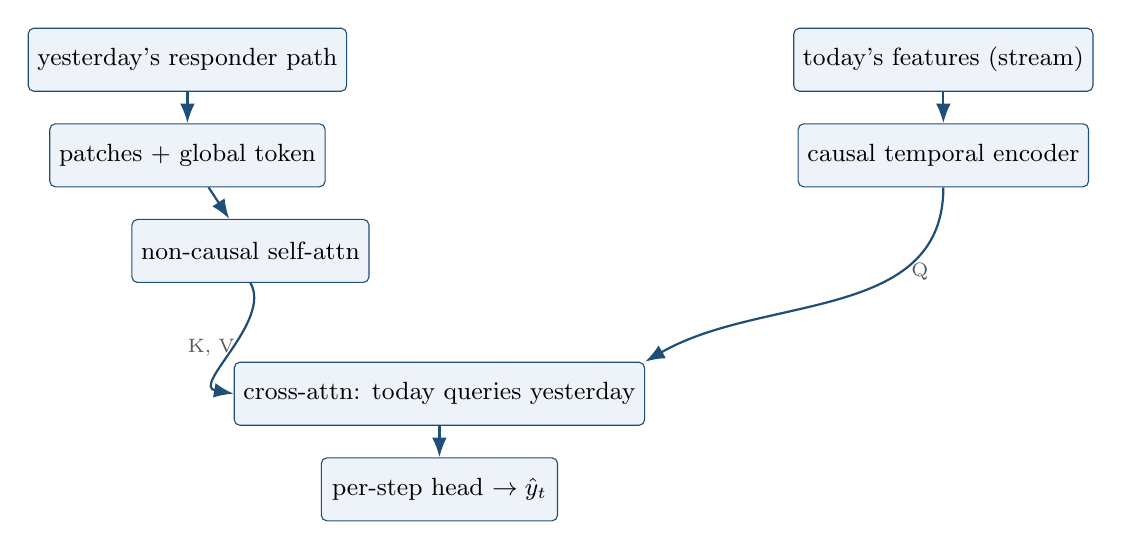
\begin{tikzpicture}[
  box/.style={draw=inkblue, fill=paleblue, rounded corners=2pt,
              minimum height=8mm, minimum width=30mm, font=\small},
  arr/.style={-{Latex[length=2.5mm]}, thick, color=inkblue}]
\node[box] (endo) at (0,0) {yesterday's responder path};
\node[box, below=4mm of endo] (patch) {patches + global token};
\node[box, below=4mm of patch, xshift=8mm] (selfa) {non-causal self-attn};
\node[box] (exo) at (9.6,0) {today's features (stream)};
\node[box, below=4mm of exo] (caus) {causal temporal encoder};
\node[box, below=10mm of selfa, xshift=24mm] (bridge)
  {cross-attn: today queries yesterday};
\node[box, below=4mm of bridge] (head) {per-step head $\to \hat y_t$};
\draw[arr] (endo) -- (patch);
\draw[arr] (patch) -- (selfa);
\draw[arr] (exo) -- (caus);
\draw[arr] (selfa.south) to[out=-60,in=170] node[pos=0.35, below left,
  font=\scriptsize, color=inkgray] {K, V} (bridge.west);
\draw[arr] (caus.south) to[out=-90,in=30] node[pos=0.3, right,
  font=\scriptsize, color=inkgray] {Q} (bridge.north east);
\draw[arr] (bridge) -- (head);
\end{tikzpicture}
\end{center}

The general design lesson outlives this architecture: \textbf{when a paper
assumes batch access to a window and your protocol streams, do not discard
the idea --- find which stream is fully known and re-aim the attention so
information flows from the known into the causal.}

\section{The honest state of the evidence}

Where things stood at the time of writing, stated plainly because this
book's credibility rests on such statements:

\begin{itemize}
\item Vanilla causal transformer: built, measured, \textbf{kept as
  baseline only} --- statically fine, refit-inert, ensemble weight zero
  (too correlated with the RNNs; Chapter~\ref{ch:ensembling}).
\item Causal iTransformer and TimeXer: \textbf{built, causality-audited,
  not yet conclusively benchmarked} --- their fair evaluation needs GPU
  budgets our laptop phase did not have, and one interrupted CPU run
  proves nothing either way.
\item To decide whether they \emph{deserve} the GPU budget, we built the
  synthetic triage world of Chapter~\ref{ch:synthetic}: planted mechanisms
  matched to each bias (a yesterday-path $\times$ time-of-day effect for
  TimeXer; persistent cross-variate min-gates for iTransformer) at the
  real problem's SNR, with reference-predictor ceilings. The decision
  rule, fixed before results: \emph{an architecture that cannot beat the
  GRU on a world designed for its own inductive bias does not get real
  compute.}
\end{itemize}

\section{When attention should win (and when it shouldn't)}

Collecting the chapter into a decision surface:

\begin{itemize}
\item \textbf{Attention over time} pays when long-range, content-dependent
  retrieval matters (``find the last time the day looked like this
  morning''). At $R^2 = 0.01$, with 968-step days whose early context an
  RNN summarizes adequately, we found no measurable retrieval premium ---
  and a real adaptation penalty.
\item \textbf{Attention over variates} pays when cross-feature structure
  is rich and state-dependent --- which forensics says is true here. It
  is the more promising direction of the two, and the cheaper one (tokens
  = a dozen selected variates, not 968 steps).
\item \textbf{The endo/exo split} pays when the protocol makes the
  target's history a \emph{differently-shaped} input than the covariates
  --- as daily lag delivery does. It is a protocol-shaped bias, which is
  the best kind.
\item All of it must survive the two genre taxes: the \textbf{adaptation
  tax} (does daily refit help it? at what learning rate ---
  Chapter~\ref{ch:online}'s cliffs are family-specific) and the
  \textbf{correlation tax} (does its stream decorrelate from the RNNs
  enough to earn ensemble weight? --- Chapter~\ref{ch:ensembling}).
  The vanilla transformer failed both. The two structured variants get
  their verdict from the synthetic world first.
\end{itemize}

\begin{drillbox}
Take any published forecasting architecture and perform the streaming
audit we performed on TimeXer: list every tensor it builds; mark which
would contain future values under a one-step-at-a-time protocol; redesign
the minimal set of attention directions so all flows go from
fully-known to causal. If no such redesign exists, the architecture is
batch-only --- knowing that before implementation is the cheapest
experiment you will ever run.
\end{drillbox}

\chapter[Path Signatures]{The Model Zoo IV: Path Signatures --- a Beautiful Negative Result}
\label{ch:signatures}

This chapter is a full post-mortem of an idea that was mathematically
elegant, correctly implemented, individually competitive --- and added
nothing. We include it at chapter length deliberately: the failure mode it
illustrates (\emph{redundancy with an existing model family}) is one of the
genre's most expensive lessons, and the machinery itself remains worth
knowing for problems shaped differently than this one.

\section{The mathematics, briefly}

The \textbf{signature} of a path $X: [0, T] \to \mathbb R^d$ is the
sequence of iterated integrals
\[
S^{(i_1, \dots, i_k)}(X) \;=\;
\idotsint\limits_{0 < t_1 < \cdots < t_k < T}
dX^{(i_1)}_{t_1} \cdots\, dX^{(i_k)}_{t_k},
\qquad k = 1, 2, \dots
\]
collected over all index words $(i_1,\dots,i_k)$. Level 1 gives net
increments; level 2 encodes pairwise areas (which coordinate led which);
higher levels encode progressively finer order-of-events geometry. Two
properties make signatures theoretically seductive for us:

\begin{itemize}
\item \textbf{Universality}: continuous functionals of a path are
  approximated by \emph{linear} functionals of its signature --- a
  canonical, model-free feature map for sequences.
\item \textbf{Compression of order information}: exactly the ``what
  happened, in what order, how fast'' content that intraday context
  consists of.
\end{itemize}

Practical refinements we implemented (in \code{janestreet.theory
.signatures}): truncation at depth 2--3 over $\le 8$ selected channels
(the level-$k$ term count grows as $d^k$); the \textbf{log-signature} in a
Lyndon-word basis (removes algebraic redundancy among signature terms);
and a \textbf{Volterra/Hurst reweighting} --- multiplying increments by
$(t - s)^{H - 1/2}$ before integration --- so that recent path segments
dominate, mimicking rough-kernel memory with $H \approx 0.1$.

\section{What we built and what it scored}

The signature block computed, per timestep, the (log-)signature of the
trailing window (16--64 steps) of selected feature channels, and fed it as
extra inputs to either an MLP (\code{mlp\_sig}) or a causal transformer
(\code{sig\_transformer}). Channel selection mattered and taught its own
lesson:

\begin{itemize}
\item Selecting channels by \emph{univariate target correlation} made
  things \textbf{worse} than an arbitrary default ($+0.0044$ vs
  $+0.0049$): the signature's value lives in cross-channel monomials of
  \emph{path-rich} series, not in marginally predictive ones ---
  a screen aimed at the wrong property.
\item Selecting by an \textbf{autoregressive criterion} --- ridge-fit each
  feature's own lags against the target, rank by that $R^2$ --- found
  channels whose \emph{paths} carry information: $+0.0059$ static, the
  best signature variant. (Echo of Chapter~\ref{ch:selection}: the screen
  must match the mechanism.)
\item The refit-learning-rate cliff bit hard here first: at the RNNs'
  refit lr the sig-transformer \emph{lost} $0.0015$ online, and at
  $10\times$ smaller it gained $+0.0004$ --- the diagnosis that became
  Chapter~\ref{ch:online}'s family-specific-cliff law. Final best:
  $+0.0062$ online.
\end{itemize}

$+0.0062$ is a respectable single model --- above XGB, below the RNNs.
Then came the only test that matters for a marginal family:

\section{The ensemble verdict}

Added to the standing three-stream ensemble (xgb + two online RNNs,
$+0.0104$):

\begin{center}
\begin{tabular}{@{}lr@{}}
\toprule
ensemble & $\Rw$ \\
\midrule
3-way (incumbent) & $+0.0104$ \\
+ sig-transformer stream (4-way average) & $+0.0101$ \\
optimal-weight blend, 4 streams & assigns signature weight $\approx 0$ \\
\bottomrule
\end{tabular}
\end{center}

The signature stream's predictions correlated with the RNN streams tightly
enough that averaging it in \emph{diluted} the blend. The information the
signature extracts from an intraday window --- increments, leads/lags,
order-of-events geometry --- is evidently a subset of what a gated RNN's
hidden state already carries by that point in the day. The mathematics is
not wrong; it is \emph{redundant given the incumbents}.

\begin{keybox}[: elegance is not additivity]
The question for any new family is never ``is it good?'' but ``is it good
\emph{and decorrelated from what I have}?''
(Chapter~\ref{ch:ensembling}'s admission rule). A solo score can be earned
by re-deriving information the ensemble already owns; only decorrelated
error buys anything. Probe correlation \emph{before} polishing: two seeds,
small config, correlate the validation prediction stream against each
incumbent --- an afternoon that would have saved us several weeks.
\end{keybox}

\section{Where signatures still belong}

The machinery survives in the repository (\code{janestreet.theory}), and
the honest map of where it should pay:

\begin{itemize}
\item \textbf{No recurrent incumbent}: pipelines built on trees/MLPs only
  (many production settings) --- signature features are the cheapest way
  to hand path geometry to a stateless model; our \code{mlp\_sig} at
  $+0.0066$ beat XGB with zero recurrence.
\item \textbf{Short, irregular, or event-driven sequences} where RNN state
  has nothing to accumulate but path geometry still discriminates
  (medical time series, sensor bursts).
\item \textbf{As a screen}: the AR-based channel selector we built for
  signatures outlived them --- it is a general ``whose \emph{path} is
  informative?'' ranking, complementary to the atlas.
\end{itemize}

\section{Post-mortem: the process failure, not the math failure}

The reconstruction of how a wrong bet stayed alive for weeks, because the
pattern is general:

\begin{enumerate}
\item \textbf{Solo-score progress masked ensemble irrelevance.} Each
  iteration improved the signature model against itself; nobody re-ran the
  correlation probe until late.
\item \textbf{A confounded failure was mis-attributed.} The online-refit
  regression looked ``architectural'' for two runs before the lr sweep
  revealed a tuning cliff --- during which time the family's stock was
  wrongly discounted, muddying decisions.
\item \textbf{Sunk elegance.} The mathematics was a pleasure, and pleasure
  is a bias. The eventual kill decision was made by one number (blend
  weight $\approx 0$) that had been computable from week one.
\end{enumerate}

The repaired process --- decorrelation probe first, family-specific lr
sweep before any online verdict, kill criteria written down in advance ---
is codified in Chapters~\ref{ch:online}, \ref{ch:ensembling}, and
\ref{ch:diagnostics}. That is what a negative result is \emph{for}.


\part{Training and Operations}
\chapter{Online Learning: The Biggest Lever}
\label{ch:online}

If this book had to be compressed to one operational sentence, it would be:
\emph{in a drifting environment with delayed labels, a small daily gradient
step is worth more than any architecture you will try.} This chapter
quantifies that claim, derives the protocol, and maps the cliffs.

\section{The setting: delayed labels are an invitation}

The competition's lag mechanism --- yesterday's full responder table
delivered every morning (Chapter~\ref{ch:problem}) --- is not just a
feature source. It is a supervision stream: every day, 968 labeled steps
per symbol arrive, drawn from \emph{the most recent regime in existence}.
A frozen model ignores them; an adaptive one converts them into score.

The measured conversion rate, on our standard harness:

\begin{center}
\begin{tabular}{@{}lrrr@{}}
\toprule
model & static & online & $\Delta$ \\
\midrule
gru (single branch) & $+0.0025$ & $+0.0075$ & $+0.0050$ \\
gru\_modelr & $+0.0076$ & $+0.0089$ & $+0.0013$ \\
lstm\_modelr & $+0.0064$ & $+0.0092$ & $+0.0028$ \\
transformer & $+0.0047$ & $+0.0050$ & $+0.0003$ \\
sig-transformer (right lr) & $+0.0059$ & $+0.0062$ & $+0.0004$ \\
sig-transformer (RNN's lr) & $+0.0059$ & $+0.0044$ & $\bm{-0.0015}$ \\
\bottomrule
\end{tabular}
\end{center}

Three facts jump out, and the rest of the chapter unpacks them: the effect
is \textbf{large} (up to $+0.005$ --- compare the whole competitive range
of $0.012$); it is \textbf{family-dependent} (RNNs feast, attention
nibbles); and it can go \textbf{catastrophically negative} under
mis-tuning.

\section{The protocol}

One correct loop, matching deployment exactly
(Chapter~\ref{ch:validation}):

\begin{enumerate}
\item For each day $d$ of the evaluation walk, in calendar order:
\item \quad receive day $d{-}1$'s labels; form the day-batch
  (all symbols, all 968 steps);
\item \quad take one gradient step on the weighted-$R^2$ loss of that
  batch at learning rate $\eta_{\text{refit}}$, gradient-clipped;
\item \quad predict day $d$ causally; score; continue.
\end{enumerate}

Design choices inside that loop that we tested or inherited:

\begin{itemize}
\item \textbf{One step, not convergence.} The daily batch is one noisy
  draw from a moving distribution; fitting it well is overfitting it.
  A single clipped step is a \emph{tracking} update --- exponential
  smoothing in weight space.
\item \textbf{Which loss:} refit on the \emph{target} head only
  (the reference solution refits on \resp{6} alone, not the auxiliary
  heads). The aux heads did their job shaping the representation offline;
  online, you chase the target.
\item \textbf{Fresh optimizer state.} Our \code{update()} constructs the
  optimizer anew each day --- no stale Adam moments carried across a
  regime. With one step per day, momentum has nothing useful to
  accumulate anyway; a clean clipped step at the right $\eta$ is easier to
  reason about and measured fine.
\item \textbf{The scaler adapts too} (Chapter~\ref{ch:preprocessing}) ---
  but only from already-predicted days, and its setting is frozen during
  lr sweeps to keep the experiment single-variable.
\end{itemize}

\section{The learning-rate cliffs: a family-specific law}

The central empirical finding. Sweeping $\eta_{\text{refit}}$ per family:

\begin{center}
\begin{tabular}{@{}lrr@{}}
\toprule
$\eta_{\text{refit}}$ & lstm\_modelr & sig-transformer \\
\midrule
$0$ (static) & $+0.0063$ & $+0.0059$ \\
$10^{-5}$ & --- & $+0.0061$ \\
$3\times10^{-5}$ & --- & $\bm{+0.0062}$ \\
$10^{-4}$ & $+0.0083$ & $+0.0061$ \\
$3\times10^{-4}$ & $+0.0091$ & $+0.0044$ \\
$10^{-3}$ & $\bm{+0.0092}$ & $-0.0090$ \\
$3\times10^{-3}$ & $+0.0070$ & --- \\
\bottomrule
\end{tabular}
\end{center}

Read the columns separately, then together:

\begin{itemize}
\item Each family has a \textbf{plateau} (roughly a decade wide) flanked
  by cliffs: too small wastes the labels, too large lets one day's noise
  scramble the network ($-0.009$ is not a typo; that is a destroyed
  model).
\item The plateaus are \textbf{30$\times$ apart} between families
  ($10^{-3}$ vs $3\times10^{-5}$). A default tuned on one family sits on
  the other's cliff.
\item Consequence for research process: \textbf{no online-behavior verdict
  about an architecture is valid until its own lr sweep has run.} We
  spent two runs believing ``signature-transformers regress under refit''
  --- an architectural-sounding conclusion that was actually a borrowed
  hyperparameter (the full post-mortem is \S\ref{ch:signatures}).
\end{itemize}

\begin{warnbox}[: the borrowed-hyperparameter fallacy]
Whenever a new family underperforms under a procedure tuned on an old
family, the procedure's hyperparameters are confounded with the
architecture. Sweep before concluding. This fallacy has a long history in
deep learning (``X doesn't work'' $\to$ ``X needed its own lr'') and at
low SNR it is nearly undetectable without a deliberate sweep, because all
the numbers involved are small.
\end{warnbox}

\section{Why recurrence adapts best: a working hypothesis}

The pattern --- RNNs gain 10$\times$ more from identical updates --- wants
an explanation. Ours, offered as hypothesis with its supporting
observations: a gated RNN's function is \emph{smoothly} parameterized
(small weight changes $\to$ small, well-conditioned changes in its
temporal filtering), so a single clipped step moves it a small, useful
distance. Attention's computation routes through softmax comparisons;
identical step sizes can reorganize retrieval patterns discontinuously,
so safe steps must be tiny --- and tiny steps track drift slowly.
Consistent with this: the attention families' plateaus are both lower
\emph{and} narrower, and their best online gains ($+0.0004$) resemble a
strongly damped version of the RNN effect. Whatever the mechanism's true
name, the operational rule stands: \textbf{if online adaptation is
available, weight your architecture portfolio toward families that can
use it.}

\section{Variations we tested or queued}

\begin{itemize}
\item \textbf{Recency window + refit} (tested): the two compose --- train
  on the recent 280--400 days, \emph{and} refit daily. The window sweep's
  knee (50 $\to$ 400 days: $+0.0032 \to +0.0071$ online for the plain GRU)
  shifts \emph{up} at every length once refit is on; neither replaces the
  other.
\item \textbf{Refit-lr decay schedules} (queued): a per-day decay
  ($\eta_d = \eta_0 \cdot 0.5^{d/h}$) interpolates between adaptation and
  stability across a long test period; expected small positive by
  analogy, unproven here.
\item \textbf{Curriculum warm-starts across history} (tested, negative):
  chronologically warm-starting through 800 days of history scored
  \emph{below} the plain recent-window model ($+0.0077$ vs $+0.0089$).
  Old regimes are not a curriculum; they are interference
  (Chapter~\ref{ch:negative}).
\item \textbf{Nightly full retrains} (industry practice, out of
  competition scope): the heavyweight sibling of the daily step ---
  retrain on the trailing window every $k$ days. Composes with, does not
  replace, the light daily step.
\end{itemize}

\begin{jsbox}[: the lever in context]
Total spread from architecture choice among our serious single models:
$\sim 0.002$. Total spread from online refit on one architecture:
$\bm{0.003}$ (static $\to$ tuned online). Total spread from the refit
lr within one architecture: $\bm{0.018}$ ($-0.009$ to $+0.0092$).
The hyperparameter of the \emph{procedure} dwarfs the choice of the
\emph{model}. Allocate tuning attention accordingly.
\end{jsbox}

\begin{drillbox}
Extend Chapter~\ref{ch:rnn}'s drill: add a second architecture (any small
transformer) to your miniature drifting-panel setup and sweep refit lr
for both on a log grid from $10^{-5}$ to $10^{-2}$. Plot both curves on
one axis. You should see displaced plateaus and at least one
crossed-cliff configuration --- the borrowed-hyperparameter fallacy,
reproduced on your desk for the cost of twenty minutes of compute.
\end{drillbox}

\chapter[Training Diagnostics]{Training Diagnostics: What Learning Looks Like at
\texorpdfstring{$R^2 = 0.01$}{R2 = 0.01}}
\label{ch:diagnostics}

Most practitioners' instincts about training curves were calibrated on
problems where models reach 90\% accuracy. Those instincts misfire badly at
$R^2 = 0.01$, in both directions: healthy runs look broken, and broken runs
look healthy. This chapter recalibrates the eyes, then gives the debugging
ladder we used when things actually were broken.

\section{Recalibrating: numbers that look wrong but are right}

\begin{itemize}
\item \textbf{The loss barely moves --- forever.} Training on
  $1 - \Rw$, a perfect model converges to $\approx 0.986$; a useless one
  sits at $1.000$. The \emph{entire dynamic range of the problem} lives
  between 1.00 and 0.98. Plot the third and fourth decimals or plot
  nothing. (Our logs print losses to five places for exactly this
  reason.)
\item \textbf{Epoch 1 is worse than doing nothing.} A freshly initialized
  network outputs nonzero noise, which scores \emph{negative} against the
  zero-origin metric (train $R^2 \approx -0.02$ is typical). It should
  cross zero within an epoch or two and creep upward. Panic only if it
  doesn't cross.
\item \textbf{Validation $R^2$ of $+0.008$ is a good model.} Internalize
  the ladder of Chapter~\ref{ch:metric}. And its converse ---
\item \textbf{validation $R^2$ of $+0.05$ is an emergency}, not a
  breakthrough: at 3--4$\times$ the known ceiling, the probability that
  you out-modeled the world's best team by that margin is far below the
  probability of a centered rolling window
  (Chapter~\ref{ch:leakage}). Our standing rule: celebrate \emph{after}
  the leak hunt fails.
\item \textbf{Train--validation gaps are structural.} Train $R^2$ of
  0.02--0.03 against validation 0.008 is the equilibrium of a correctly
  regularized model at this SNR --- memorization pressure is constant and
  nonzero. The gap is monitored for \emph{growth}, not for existence.
\end{itemize}

\section{The curves worth logging}

Beyond the loss, five series earn their disk space in every run:

\begin{enumerate}
\item \textbf{Validation weighted-$R^2$ per epoch} --- the decision
  variable for early stopping (patience $\sim$10: the curve is noisy
  enough that patience 2--3 stops on fluctuations; we measured
  best-epoch spreads of 5+ epochs across seeds of identical configs).
\item \textbf{Per-day validation score} at the end --- a distribution, not
  a number. A model that wins by $+0.02$ on three days and loses
  everywhere else is fragile in a way the mean hides; a model whose
  worst days cluster at regime events tells you what feature is missing.
\item \textbf{Prediction statistics}: mean (bias burns score
  quadratically --- Chapter~\ref{ch:metric}), standard deviation
  (collapse toward zero-variance predictions is the classic
  under-trained/over-regularized signature; explosion signals a broken
  scaler), and max $|\hat y|$ (one 50-sigma prediction on a high-weight
  row can erase a day).
\item \textbf{Gradient norms} pre-clipping --- heavy-tailed days announce
  themselves here first; a rising trend mid-training precedes most
  divergences we saw.
\item \textbf{The static/online pair} for any adaptive model
  (Chapter~\ref{ch:online}) --- the gap between them is a diagnostic
  in its own right, and its collapse is how you notice a refit-lr
  regression before it costs a week.
\end{enumerate}

\section{The debugging ladder}

When a model underperforms expectations, resist touching hyperparameters
--- at this SNR you cannot distinguish a bad lr from a broken pipeline by
staring at scores. Climb in order; each rung is cheap and conclusive:

\subsection{Rung 1: anchor the floor}

Score the trivial ensemble: all-zeros (must be exactly $0.000$ --- if not,
your metric implementation is wrong, and yes, we have seen that), plus a
10-feature ridge probe (should land $+0.002$ to $+0.004$ here). Your model
must live above both. A deep model \emph{below the linear probe} has a
wiring problem, not a capacity problem.

\subsection{Rung 2: overfit on purpose}

Train on 3 days, validate on the same 3 days. Any healthy architecture
must push train $R^2$ far above the signal level ($0.2+$) by memorizing.
Failure localizes the bug precisely: data loader shapes, mask direction,
loss reduction, weight plumbing --- something mechanical. This test found
a transposed (symbol, time) batch for us in minutes; no amount of
production-scale training would have.

\subsection{Rung 3: causality and structure probes}

The shift and shuffle tests of Chapter~\ref{ch:leakage}, run as
\emph{model} diagnostics: score collapse under a one-step feature shift
$\Rightarrow$ leakage; score \emph{survival} under within-day shuffling
$\Rightarrow$ your sequence model is not using sequence (which, for an
RNN scoring near the MLP baseline, is confirmation of rung-2-class bugs
or of features that already contain all the time structure).

\subsection{Rung 4: seed replication}

Three seeds minimum before comparing anything to anything
(Chapter~\ref{ch:problem}). Our measured seed spread ($\pm 0.0003$ to
$0.0008$) is the unit of measurement; an effect inside one unit does not
exist yet.

\subsection{Rung 5: now, and only now, hyperparameters}

And even then, sweep the parameters with cliffs first (refit lr ---
Chapter~\ref{ch:online}; training lr; clipping threshold) before the
parameters with plateaus (width, depth, dropout) --- our capacity sweeps
were flat, our procedure sweeps were not.

\section{Comparing runs honestly}

The bookkeeping that turns runs into knowledge
(Chapter~\ref{ch:validation} covers the validation side):

\begin{itemize}
\item \textbf{One variable per comparison.} The temptation to bundle
  (``new features \emph{and} more width, it won!'') destroys attribution
  exactly where effects are small enough that attribution is the whole
  point.
\item \textbf{Fixed harness, forever.} Same dates, same embargo, same
  metric code, same seeds across every experiment in a campaign. All of
  this book's tables are mutually comparable because the harness never
  moved.
\item \textbf{Append-only results log} with config hashes. Selection bias
  feeds on forgotten losers (Chapter~\ref{ch:leakage}); the log is the
  immune system. Ours is a directory of JSON artifacts plus two markdown
  ledgers --- nothing fancier than that is needed.
\end{itemize}

\begin{jsbox}[: a real debugging transcript, compressed]
Symptom: sig-transformer online score $0.0044$, well below its static
$0.0059$ --- ``online refit breaks signatures.''
Rung 1--2: pass (wiring fine). Rung 3: pass (no leak; sequence used).
Rung 4: reproduces across seeds --- so it is real, but real
\emph{what}? Rung 5, cliff parameters first: refit-lr sweep $\to$ at
$3\times10^{-5}$ the regression becomes a gain ($+0.0062$).
Conclusion rewritten: not an architecture defect --- a borrowed
hyperparameter (Chapter~\ref{ch:online}). Total ladder time: one
afternoon. Time spent on the wrong conclusion before running the ladder:
two weeks of intermittent confusion.
\end{jsbox}

\begin{drillbox}
Instrument your current training script with the five curves of this
chapter, then deliberately break it four ways --- transpose two batch
dimensions, unweight the loss, center a rolling window, set refit lr
10$\times$ high --- and re-run. Learn each failure's curve signature
while the stakes are zero; at $R^2=0.01$, recognizing them from curves is
a survival skill, because the \emph{scores} of broken and healthy runs
overlap.
\end{drillbox}

\chapter{Ensembling}
\label{ch:ensembling}

Chapter~\ref{ch:problem} argued that at low SNR, estimation variance is the
dominant error term and averaging is the dominant cure. This chapter turns
that argument into procedure: what to average, how to weight, how to
manufacture diversity cheaply, and the two seductive upgrades (fitted
weights, stacking) that measured \emph{worse} than doing nothing clever.

\section{The arithmetic of averaging}

For prediction streams $\hat y^{(1)}, \dots, \hat y^{(m)}$ with equal
individual error variance $\sigma^2$ and average pairwise error correlation
$\bar\rho$, the simple average's error variance is
\[
\Var\!\Big(\tfrac{1}{m}\sum_i \varepsilon^{(i)}\Big)
= \sigma^2\Big(\frac{1-\bar\rho}{m} + \bar\rho\Big)
\;\xrightarrow{m \to \infty}\; \sigma^2 \bar\rho .
\]
Two readings, both of which drove decisions:

\begin{itemize}
\item The benefit saturates fast in $m$ but is \emph{unbounded} in
  $(1-\bar\rho)$: after three or four members, adding more of the same
  helps little, while adding something \emph{different} keeps paying.
  Diversity is the currency; member count is not.
\item A weaker model with decorrelated errors can beat a stronger clone.
  Our XGB stream scores $+0.0068$ against the LSTM's $+0.0092$, yet
  removing XGB from the blend costs more than removing the second RNN ---
  tree errors and neural errors disagree in structurally different
  places.
\end{itemize}

\begin{jsbox}[: the headline blend]
Three streams --- xgb static ($+0.0068$), gru\_modelr online ($+0.0089$),
lstm\_modelr online ($+0.0092$) --- simple average: $\bm{+0.0104}$.
The blend beats its best member by $+0.0012$, which is more than almost
any single modeling idea in this book earned. Cost of the technique:
one line of numpy.
\end{jsbox}

\section{Simple average versus fitted weights: a measured upset}

Optimal linear blending --- fit weights on held-out data --- dominates the
simple average \emph{in expectation with enough data}. At this SNR you do
not have enough data. Our measurement: weights fit on one half of the
validation tail, evaluated on the other half, \textbf{lost to the simple
average every time}, and the fitted weights themselves told the story ---
they kept collapsing into corner solutions (all weight on one stream, zero
on whole families), the classic signature of an optimizer fitting noise.
Weight estimation is itself a low-SNR regression with $m$ parameters and
one noisy signal; with 3--6 streams the estimation error exceeds the gain
over uniform weights.

Non-linear stacking (an XGB meta-model over the streams) did worse still,
for the same reason squared: more meta-capacity, same meta-noise.

\begin{keybox}[: the ensemble complexity ladder]
Climb only while a held-out set (that the weights never touched) says the
step pays: (1) simple average $\to$ (2) sign-constrained coarse weights
(e.g.\ family weights in $\{0.5, 1, 1.5\}$) $\to$ (3) fitted convex
weights $\to$ (4) stacking. In this campaign the ladder ended at rung 1.
The DRW winner's ensemble was similarly primitive: NN protagonist, XGB
seasoning. Public post-mortems of this genre are a graveyard of rung-4
blends that lost to rung 1 on private data.
\end{keybox}

\section{Manufacturing diversity}

Ranked by measured or observed cost-effectiveness in this campaign:

\begin{enumerate}
\item \textbf{Family diversity} (trees + RNN): the largest decorrelation
  per unit effort --- different function class, different failure
  geometry. This is why XGB is never dropped
  (Chapter~\ref{ch:treesmlp}).
\item \textbf{Seed diversity}: same architecture, different seeds. Cheap,
  reliable, small: the reference 8th-place solution averaged
  \emph{sixteen} seeds of one architecture. At $\pm 0.0005$ seed spread,
  averaging 4--16 seeds recovers a meaningful fraction of it.
\item \textbf{Temporal bagging}: members trained on different
  (overlapping) date subsets --- distinct regimes produce distinct
  errors, and the memmap manifest
  (Chapter~\ref{ch:preprocessing}) makes it one config line
  (\code{resample: subsample, frac 0.6}). Our infrastructure treats
  ``bag = list of (model, seed, date-resample) members'' as the unit of
  experiment.
\item \textbf{Adaptation diversity}: static and online variants of the
  \emph{same} model decorrelate on exactly the days that drift ---
  including both is nearly free since one is a byproduct of evaluating
  the other.
\item \textbf{Architecture diversity beyond family}: the expensive
  aisle, to be shopped with the admission rule below --- our signature
  and vanilla-transformer streams both failed it after substantial
  investment (Chapter~\ref{ch:signatures}).
\end{enumerate}

\section{The admission rule}

Codifying the campaign's most-regretted omission into procedure: a
candidate stream earns ensemble admission by showing, on cheap probes
(2 seeds, small config), that it is

\begin{enumerate}
\item \textbf{non-negative solo} (it clears zero robustly), and
\item \textbf{decorrelated}: prediction-stream correlation with every
  incumbent below a threshold we set at $\sim 0.9$, and --- the sharper
  test --- the incumbent blend \emph{with} the candidate beats the blend
  without it on held-out days.
\end{enumerate}

Run the probe \emph{before} polishing the candidate
(Chapter~\ref{ch:signatures}'s post-mortem: solo-score progress is a
treadmill if the stream is redundant). Notice the rule's corollary: a
mediocre-looking model can be admitted (XGB) while an impressive one is
rejected (sig-transformer, $+0.0062$ solo, blend weight zero). The
ensemble does not care about résumés.

\section{Ensembling adaptive models}

Two operational notes specific to this genre's online dimension
(Chapter~\ref{ch:online}):

\begin{itemize}
\item \textbf{Blend after adaptation, not before}: each member refits
  itself daily, then predictions are averaged. Averaging \emph{weights}
  across members (as opposed to predictions) is a different, riskier
  operation --- only valid within identical architectures, and unneeded
  here.
\item \textbf{Diversity drifts too.} Streams that decorrelate today may
  converge as they all adapt toward the same recent regime. If the test
  period is long, re-check pairwise correlations on a rolling basis ---
  in our walks the effect was visible but small; over months it might
  not be.
\end{itemize}

\section{Checklist}

\begin{enumerate}
\item Build the simple average of your best-per-family models before any
  further modeling; it is the new baseline.
\item Admit streams by the two-part rule (non-negative solo;
  decorrelation with incumbents), probed cheaply, before polishing.
\item Manufacture diversity in cost order: families, seeds, temporal
  bags, adaptation variants --- architectures last.
\item Climb the weighting ladder only while untouched held-out data says
  each rung pays; expect to stop at rung 1.
\item Keep the blend's member list short and auditable; log per-member
  and blend scores per day so a degrading member is visible.
\end{enumerate}

\chapter[Synthetic Benchmarking]{Synthetic Benchmarking: Triage Before
You Buy GPU Time}
\label{ch:synthetic}

An architecture evaluation on real data costs GPU-days and returns one
noisy bit. When forensics has recovered the shape of the data-generating
process (Part~II), a better instrument exists: \textbf{build a synthetic
world with that shape, plant mechanisms you control, compute the optimal
score in closed form, and triage architectures against the known ceiling
--- at laptop cost}. This chapter presents the method and the generator we
built (\code{scripts/synth\_bench.py}).

\section{Why synthetic tests usually lie, and how to make them honest}

The standard objection is sound: toy benchmarks reward toy strengths.
Synthetic triage earns trust only under four disciplines, each fixing a
standard failure:

\begin{enumerate}
\item \textbf{Match the SNR.} The classic sin is testing at $R^2 = 0.5$
  where clever architectures shine, then deploying at $R^2 = 0.01$ where
  regularization dominates everything. Calibrate the planted signal so
  the \emph{optimal} score sits near the real problem's ceiling (ours:
  reference $R^2 \approx 0.03$--$0.05$ against the real $0.014$ ---
  slightly generous so verdicts resolve at small data scale, and stated
  as such).
\item \textbf{Match the protocol.} Run the synthetic world through the
  \emph{identical} production harness --- same feature pipeline, same
  frozen scalers, same walk-forward with daily online refit
  (Chapter~\ref{ch:validation}). We achieve this mechanically: the
  generator writes the canonical competition file layout, so every
  existing tool runs on it unchanged.
\item \textbf{Match the information sets.} Every candidate model receives
  identical inputs (including the lagged-target features), so a win is
  attributable to the architecture and nothing else.
\item \textbf{Fix the decision rule in advance.} Ours, written before any
  run: \emph{an architecture that cannot beat the GRU on a world designed
  for its own inductive bias does not receive real-data GPU budget.}
\end{enumerate}

\section{Designing the world: one mechanism per inductive bias}

The generator simulates the recovered construction of
Chapter~\ref{ch:targets} --- per-symbol innovation series $u$, responders
as forward SMAs (4/20/120) on two noisy venues, features as noisy
descriptions of $u$'s realized path, planted at the same indices with the
same timing signatures the atlas found. Into $u$'s conditional mean we
plant four \emph{toggleable} mechanisms, each the cleanest possible target
for one architectural bias:

\begin{center}
\small
\begin{tabularx}{\textwidth}{@{}l>{\raggedright\arraybackslash}X>{\raggedright\arraybackslash}X@{}}
\toprule
mechanism & construction & should be won by \\
\midrule
\code{rev} & intraday mean reversion:
$\E[u_t] \propto -\,\mathrm{SMA}_{20}(u)_{t-1}$ & any causal temporal
model \\
\code{xd} & cross-day: yesterday's last-120 trend $\times$ a
time-of-day gate ($+$ early, $-$ late) & TimeXer's endogenous-patch
mechanism (Chapter~\ref{ch:attention}) \\
\code{gate} & $\E[u_t] \propto \min(f_a, f_b)$ of two persistent
observable factors (one idiosyncratic, one market-wide) & iTransformer's
variate attention; also what the symbolic search found on real data \\
\code{lead} & two features observe the next-4 innovations noisily
(the \feat{37}/\feat{38} analog) & anything --- the linear-Gaussian floor \\
\bottomrule
\end{tabularx}
\end{center}

The craft is in the details that make mechanisms \emph{forecastable but
not trivial}: the gate factors follow slow AR(1) dynamics
($\rho = 0.995$) so their state persists across the 20-step target window
(otherwise the mechanism is unlearnable from time $t$); the cross-day
mechanism requires \emph{composing} two inputs (yesterday's path and the
clock) that no single feature exposes; the lead features carry calibrated
noise so their optimal use is a shrinkage the model must learn.

\section{The reference predictor: score as a fraction of knowable}

For each mechanism we derive $\E[y_t \mid \mathcal F_t]$ in closed form
(exactly for \code{rev}/\code{xd}/\code{lead}; a $\rho^k$-decay
approximation for the min-gate, whose Jensen gap we accept and disclose).
The generator writes these \emph{per-mechanism oracle columns} beside the
data. Every model's score is then reported as a \textbf{fraction of the
reference}, and --- the sharper instrument --- per-mechanism attribution
is available by construction: re-generate the world with one mechanism's
coefficient zeroed and difference the scores.

\begin{keybox}[: triage reads, decided in advance]
The bench's output is a (model $\times$ world) table read against three
patterns. \emph{TimeXer $\approx$ GRU on the full world}: its bias is not
realizable at this SNR and data volume $\to$ no GPU budget --- decision
made for a laptop-hour. \emph{TimeXer $>$ GRU on full, $=$ on
xd-zeroed}: the mechanism is real and TimeXer harvests it $\to$ the
real-data question becomes ``how much \code{xd}-like structure does the
real panel have?'', which the lag ablations already bound
(Chapter~\ref{ch:featurepatterns}). \emph{Everything far below
reference}: the harness or the calibration is broken --- fix before
concluding anything about architectures.
\end{keybox}

\section{Validating the validator}

A synthetic world is itself code that can be wrong, so it must pass its
own forensics before grading anyone. Ours ships three self-checks: the
generated responders reproduce the triangular ACF ramps at the correct
cutoffs; the in-sample reference $R^2$ decomposes across mechanisms near
the calibrated targets (measured: full $+0.044$ = rev $0.014$ + xd
$0.007$ + gate $0.007$ + lead $0.011$, up to interaction terms); and the
atlas pipeline of Chapter~\ref{ch:featforensics}, run on the synthetic
world, recovers the planted feature taxonomy --- the forensic tools and
the generator audit each other.

\section{Beyond triage: the other uses}

Once the world exists, it answers questions the real data cannot:

\begin{itemize}
\item \textbf{Procedure tuning with ground truth}: refit-lr cliffs
  (Chapter~\ref{ch:online}), window sweeps, embargo sizes --- all
  measurable against a \emph{known} optimum rather than a noisy
  empirical best.
\item \textbf{Power analysis}: how many days of validation are needed to
  resolve a $+0.001$ true difference at this SNR? Simulate; the answer
  disciplines real-data conclusions
  (Chapter~\ref{ch:diagnostics}).
\item \textbf{Failure rehearsal}: inject a regime break and watch each
  family's static/online scores respond; learn the curve signatures
  cheaply.
\item \textbf{Leakage fire drills}: deliberately leak (center a window,
  drop the embargo) and confirm your audit protocol catches it. An
  audit that has never caught a planted leak is untested equipment.
\end{itemize}

\begin{drillbox}
Write the minimal version for your own problem: (1) simulate the
construction your forensics recovered, at matched SNR; (2) plant one
mechanism per architecture you are weighing; (3) derive or approximate
the reference predictor and \emph{calibrate} until its score sits near
your real ceiling; (4) run your production harness unchanged. Budget a
day. Compare that to the GPU-weeks of undirected architecture search it
replaces --- and note that the discipline of step 3 will, by itself,
teach you more about your problem's knowable fraction than most modeling
weeks do.
\end{drillbox}


\part{The Campaign}
\chapter{The Campaign: A Worked End-to-End Case Study}
\label{ch:casestudy}

Methodology chapters present knowledge in its cleaned-up, logical order.
Real campaigns happen in a different order --- with dead ends, revisions,
and decisions made under uncertainty. This chapter replays ours
chronologically, because the \emph{sequencing} of effort is itself a
transferable skill, and because seeing where the score actually came from
is the best antidote to architecture romanticism.

\section{Phase 0: replicate a known-good solution}

We began not with our own ideas but by \textbf{faithfully replicating the
8th-place solution} (whose author published code and a write-up):
her feature engineering (Chapter~\ref{ch:featurepatterns}), her
multi-branch GRU (Chapter~\ref{ch:rnn}), her walk-forward protocol with
online refit (Chapter~\ref{ch:validation}), down to hyperparameters.

Why replication first is the right opening move:

\begin{itemize}
\item It \textbf{calibrates the harness}: until your pipeline reproduces a
  published number, every measurement it emits is suspect. Ours
  reproduced her tier of performance, which certified the metric
  implementation, the leakage boundaries, and the evaluation loop in one
  stroke.
\item It \textbf{front-loads infrastructure}: the replica forced the
  memmap precompute, the day-batch layout, the online-refit loop --- all
  of which every later experiment reused.
\item It \textbf{establishes the real baseline}: not ``zero'' but ``what
  a gold-tier competitor achieves,'' making every subsequent delta
  meaningful.
\end{itemize}

\section{Phase 1: benchmarks and the first surprises}

A structured benchmark over the model zoo on shared slices produced the
ladder of Chapter~\ref{ch:metric} and three early findings that set
strategy:

\begin{itemize}
\item \textbf{Data beats capacity}: 200 $\to$ 280 training days lifted
  every model; doubling width lifted nothing. Effort re-routed from
  architecture tuning to data logistics.
\item \textbf{Online refit is the lever} ($+0.003$--$0.005$ on RNNs) ---
  and the refit-lr sweep found the plateau-and-cliffs law
  (Chapter~\ref{ch:online}).
\item \textbf{The ensemble wall}: signature and transformer streams,
  despite respectable solo scores, took zero weight in blends. Diversity,
  not solo score, became the admission criterion
  (Chapter~\ref{ch:ensembling}).
\end{itemize}

Standing at $+0.0104$ with a three-stream blend --- roughly 8th-place
tier on our local protocol.

\section{Phase 2: the recalibration}

A check of the actual private leaderboard rewrote the strategy document.
We had been benchmarking against $+0.0112$ --- the 8th place's
\emph{public} score; the private reality: 8th $= 0.0104$, 1st
$= \bm{0.0139}$, with a conspicuous gap between the top three
(0.0132--0.0139) and the pack (4th at 0.0117). Two conclusions:

\begin{itemize}
\item Our local $+0.0104$ was already 8th-tier --- the replication had
  succeeded more fully than assumed.
\item The top three, none of whom published, were separated from the pack
  by a margin ($\sim +0.002$) too large for ensemble polish. They likely
  had \emph{structural} insight the pack lacked. Chasing them with more
  bagging was arithmetic denial; the campaign pivoted to forensics.
\end{itemize}

\begin{keybox}[: read the leaderboard as evidence]
The \emph{shape} of a final leaderboard is data about the problem.
A smooth continuum says grind and variance reduction; a step
discontinuity, like this one's after 3rd place, says a discrete idea
exists that the pack missed. Aim accordingly.
\end{keybox}

\section{Phase 3: the forensic pivot}

In one stretch, the campaign built and ran the instruments of Part~II:
the deconvolution of \resp{8} into the underlying signal
(\S\ref{sec:deconv}, validated by its three sanity checks), the lead--lag
atlas over all 79 features (\S\ref{sec:atlas}), and the two-window
stability gate. Yield, within days:

\begin{itemize}
\item the feature taxonomy (lead / reversal / slow-SMA / market-wide),
  stable at Spearman $+0.97$ across 600 days;
\item the discovery that three features arrive pre-smoothed (SMA-160
  fingerprints) --- an un-smoothing opportunity
  (Chapter~\ref{ch:smoothing});
\item nowcast auxiliary heads (\S\ref{sec:auxtargets}), implemented and
  queued for GPU A/B;
\item and the seeds that upgraded the DRW-style symbolic search from
  $+0.00039$ to $+0.00052$ (Chapter~\ref{ch:selection}).
\end{itemize}

The contrast with Phase 1 is the book's thesis in miniature: a month of
architecture benchmarking moved the blend by $\sim +0.001$; days of
forensics generated the entire remaining research agenda.

\section{Phase 4: importing another competition's playbook}

The DRW crypto winner's write-up was ported wholesale
(Chapter~\ref{ch:selection}): correlation-medoid pruning,
SHAP-consistency, symbolic recombination, with our forensic corrections
(skip pruning on curated pools; seed the search from the atlas). Measured
value on the fixed harness: $+0.0005$ --- and, as a byproduct, the
discovery that the strongest combinations were market-gated reversal
terms, itself a new forensic fact.

The meta-lesson: \textbf{solution write-ups from adjacent competitions
are importable technology}. Reading them is cheap; porting them onto your
own harness --- with your own ablation discipline, because boundary
conditions differ --- is a reliably positive-expected-value activity.

\section{Phase 5: disciplined architecture bets}

Only in the final phase, with forensics in hand, did the campaign return
to architectures --- now as \emph{targeted} bets rather than a zoo tour.
The causal iTransformer and inverted-bridge TimeXer
(Chapter~\ref{ch:attention}) were built because the atlas and the
symbolic search had produced specific evidence for cross-variate gates
and a natural endo/exo split. And rather than buying GPU-weeks on faith,
the synthetic triage world (Chapter~\ref{ch:synthetic}) was built to
decide, at laptop cost, whether either bias is realizable at this SNR
--- with the decision rule fixed in advance.

\section{Where the score actually came from}

The campaign ledger, consolidated. Approximate contributions to the final
local blend of $+0.0104$ (and the queued upside beyond it):

\begin{center}
\small
\begin{tabularx}{\textwidth}{@{}>{\raggedright\arraybackslash}Xr@{}}
\toprule
source & contribution \\
\midrule
replicated baseline (features + ModelR + protocol) & $+0.0076$ \\
online refit, tuned per family & $+0.0016$ \\
recency window (280--400 days vs.\ naive full history) & $+0.0012$ \\
three-stream ensemble over best-per-family & $+0.0012$ \\
engineered blocks (rsig, clusters, symbolic combos)$^{\ast}$ &
$+0.0005$--$0.0009$ \\
architecture changes beyond the replica & $\approx 0$ \\
\midrule
queued: nowcast heads, atlas-seeded features at scale, AE factors,
triaged attention & unknown \\
\bottomrule
\end{tabularx}
\end{center}
{\footnotesize $^{\ast}$measured on the XGB stream; blend-level
contribution partially overlapping with ensemble line.}

Read the zero in that table again: \emph{every} architecture beyond the
replicated one --- transformers, signatures, width doublings ---
contributed nothing to the blend that mattered. The score came from
process (adaptation, recency, averaging), features, and calibration.
That is not an argument against architecture research; it is an argument
for sequencing it \textbf{last}, behind forensics, on specific evidence,
through cheap triage.

\begin{drillbox}
Write the phase plan for your next competition before touching data, with
exit criteria per phase: (0) replicate something published --- exit when
your harness reproduces its number; (1) benchmark families on a fixed
harness --- exit at the ensemble wall; (2) recalibrate against the true
target --- exit with a gap analysis; (3) forensics --- exit with a
stability-gated taxonomy; (4) import adjacent playbooks; (5) targeted
architecture bets through synthetic triage. Then notice how much of the
usual first month --- architecture shopping --- this plan defers, and
where it spends the time instead.
\end{drillbox}

\chapter[The Graveyard of Negative Results]{The Graveyard: Negative Results, Properly Buried}
\label{ch:negative}

A negative result that is written down with its evidence is an asset: it
prunes the search space forever. One that is merely remembered gets
re-litigated every time enthusiasm returns. This chapter is our graveyard
--- each entry with the tombstone (what died), the autopsy (why), and the
epitaph (the general rule it purchased). Scores are weighted $R^2$ on the
standard harness.

\section{Training on more history}

\textbf{Tombstone.} Curriculum training across 800 days of history:
$+0.0077$, \emph{versus} $+0.0089$ for the same architecture on the recent
280 days. Old-data models' \emph{static} scores on the recent tail were
frequently negative. The window sweep (50/100/200/400 days $\to$
$+0.0032/+0.0054/+0.0059/+0.0071$ online) rises toward a knee and the
full-history point falls off it.

\textbf{Autopsy.} Drift (\S\ref{sec:drift}): old regimes teach
feature--target relationships that no longer hold, and at low SNR the
model cannot tell stale structure from current structure --- extra rows
add interference, not information.

\textbf{Epitaph.} \emph{More data is not a default good under drift; the
training window is a hyperparameter with a knee. Sweep it.}

\section{Symbol identity as a feature}

\textbf{Tombstone.} One-hot symbol id into XGB: $-0.00002$.

\textbf{Autopsy.} Per-symbol rolling normalization
(Chapter~\ref{ch:preprocessing}) had already removed the per-symbol level
--- identity's main content. Thirty-nine dummy columns bought tree splits
and nothing else. The salvageable remainder was the \emph{stable} coarse
grouping: feature-profile clusters (+0.00022).

\textbf{Epitaph.} \emph{Before adding a feature, ask what your
normalization already removed. Identity features prosper only where
identity-linked structure survives preprocessing --- and is stable.}

\section{Symbol clustering by responder co-movement}

\textbf{Tombstone.} Clusters computed on one window looked excellent
(intra/inter co-movement ratio $\sim$18$\times$); recomputed on a later
window, agreement with the earlier clustering was ARI $= -0.07$ ---
chance. The planned per-cluster specialist models were cancelled without
training one.

\textbf{Autopsy.} Co-movement structure in this panel is
regime-transient. A routing scheme built on it routes tomorrow's symbols
by yesterday's dead map.

\textbf{Epitaph.} \emph{Any structure you intend to build on must first
pass a cross-window stability gate (\S\ref{sec:atlas}). Ten minutes of
checking beats weeks of specialist models. Compare the atlas: same gate,
Spearman $+0.97$ --- build on that instead.}

\section{Raw lagged responders as flat features}

\textbf{Tombstone.} Nine previous-day responder columns into XGB:
$-0.00003$.

\textbf{Autopsy.} As \emph{levels} at matched clock time, yesterday's
moving averages carry almost no linear information about today's value
(the construction: MAs of near-white innovations). Their content is
relational --- differences across windows and venues ($+0.0003$ as the
rsig block) or sequential (as inputs to a recurrent/endogenous stream).

\textbf{Epitaph.} \emph{A dead feature is often a live feature wearing
the wrong parameterization. Consult the construction before discarding
the information} (Chapter~\ref{ch:featurepatterns}).

\section{Bigger models}

\textbf{Tombstone.} LSTM width doubled (0.9M $\to$ 1.6M parameters):
score change within seed noise. Depth additions: same.

\textbf{Autopsy.} The binding constraints are the signal budget and
estimation variance, not expressiveness
(Chapter~\ref{ch:problem}). Capacity beyond ``enough'' buys variance.

\textbf{Epitaph.} \emph{At low SNR, capacity sweeps are flat and
procedure sweeps are not (Chapter~\ref{ch:online}). Spend tuning hours
where the curvature is.}

\section{Signature models as ensemble members}

\textbf{Tombstone.} Best signature variant $+0.0062$ solo; ensemble
weight $\approx 0$; 4-way average \emph{below} the 3-way ($+0.0101$ vs
$+0.0104$). Full post-mortem: Chapter~\ref{ch:signatures}.

\textbf{Epitaph.} \emph{Admission is decorrelation, not solo score. Probe
correlation before polishing.}

\section{Non-linear stacking and fitted blend weights}

\textbf{Tombstone.} Fitted convex weights: corner solutions, lost to the
simple average on held-out halves. XGB meta-stacker: worse.

\textbf{Autopsy.} Weight fitting is itself low-SNR estimation; with a
handful of streams the estimation error exceeds the edge over uniform
(Chapter~\ref{ch:ensembling}).

\textbf{Epitaph.} \emph{The ensemble ladder is climbed only while
untouched data pays you to climb; expect rung one.}

\section{Univariate correlation as a feature screen}

\textbf{Tombstone.} Signature channels ranked by $|\corr(x, y)|$
underperformed an arbitrary default ($+0.0044$ vs $+0.0049$); lag
columns, valuable in combination, score zero on the same screen and were
nearly lost to it (Chapter~\ref{ch:selection}).

\textbf{Autopsy.} The screen conflates nowcast with lead
(\S\ref{sec:atlas}) and is blind to interaction-only value.

\textbf{Epitaph.} \emph{Match the screen to the mechanism you are
selecting for: timing screens for timing (atlas alpha bands), path
screens for path models (AR-based), tree-gain screens for interactions.}

\section{A borrowed refit learning rate}

\textbf{Tombstone.} ``Online refit breaks signature-transformers'' ---
believed for two runs; actually a $10\times$ lr mismatch; at
$3\times10^{-5}$ the regression became a gain
(Chapter~\ref{ch:online}).

\textbf{Epitaph.} \emph{No cross-family conclusion is valid while a
procedure hyperparameter is borrowed. Sweep first, conclude second.}

\section{What the graveyard is for}

Notice the pattern across tombstones: almost every death was caused by
one of four recurring pathogens --- \textbf{drift} (sections 1, 3),
\textbf{already-normalized-away information} (2, 4), \textbf{low-SNR
estimation variance} (5, 6, 7), and \textbf{confounded procedure
hyperparameters} (8, 9). The graveyard is not a list of things that are
false; it is the empirical fingerprint of this genre's four ways of
fooling you. When your next idea dies, check which pathogen got it ---
and when your next idea \emph{succeeds}, check the same list before
believing it.

Maintain your own graveyard file from day one
(\code{WHAT\_DIDNT\_WORK.md} in our repository). The discipline costs a
paragraph per burial. It pays every time a promising-looking corpse
knocks on the door wearing a new hat --- which, over a long campaign, is
weekly.


\appendix
\part{Appendices}
\chapter{The Condensed Checklist}
\label{app:checklist}

The whole book as an operational sequence. Each item cites its chapter.

\section*{Before modeling}
\begin{enumerate}[label=\arabic*., itemsep=1pt]
\item Locate the metric's zero point and the realistic ceiling; write both
  at the top of your notes. (Ch.~\ref{ch:problem}, \ref{ch:metric})
\item Read the metric's formula character by character; reimplement it
  yourself; push weights into every loss and every early-stopping
  criterion. (Ch.~\ref{ch:metric})
\item Fingerprint every target: ACF shape (ramps? cutoffs?), spectrum
  (nulls? floors?), shift scan ($R^2$ vs.\ relative lag).
  (Ch.~\ref{ch:targets})
\item Fingerprint every feature the same way; build the lead--lag atlas
  against the (deconvolved) reference signal; split lead from nowcast.
  (Ch.~\ref{ch:featforensics})
\item Pass every structural finding through the two-window stability gate
  before it becomes load-bearing. (Ch.~\ref{ch:featforensics},
  \ref{ch:negative})
\item Write the deployment information set as one formal sentence; derive
  the forensic report and the dead-ends list. (Ch.~\ref{ch:leakage},
  \ref{ch:targets})
\end{enumerate}

\section*{Data discipline}
\begin{enumerate}[label=\arabic*., itemsep=1pt, resume]
\item Type every feature: trailing / contemporaneous / forward; forward
  types are targets only. Lags via date-shifted joins.
  (Ch.~\ref{ch:leakage})
\item Fit all preprocessing on training dates only; freeze at the
  boundary; online updates from predicted-past days only.
  (Ch.~\ref{ch:preprocessing})
\item Embargo $\ge$ the pipeline's longest forward reach --- labels
  included. (Ch.~\ref{ch:leakage})
\item Walk-forward validation that includes the adaptation procedure;
  static and online scores reported separately.
  (Ch.~\ref{ch:validation})
\item Establish CV--LB correlation with a handful of spread-out probe
  submissions before trusting either. (Ch.~\ref{ch:validation})
\item Measure your seed noise; effects inside one seed-noise unit do not
  exist yet. Two-tier validation; pre-registered experiments;
  append-only log. (Ch.~\ref{ch:problem}, \ref{ch:diagnostics})
\item Precompute features once; float16 storage / float32 compute;
  memmap with a date-range manifest; rows ordered by access pattern.
  (Ch.~\ref{ch:preprocessing})
\end{enumerate}

\section*{Features}
\begin{enumerate}[label=\arabic*., itemsep=1pt, resume]
\item Decompose, don't destroy: level + innovation; market +
  idiosyncratic; keep both parts. (Ch.~\ref{ch:smoothing},
  \ref{ch:preprocessing})
\item Never smooth a timing signal; difference or deconvolve
  pre-smoothed series at their detected window.
  (Ch.~\ref{ch:smoothing})
\item Build the cross-sectional block (market averages, ranks) --- the
  no-latency direction. (Ch.~\ref{ch:featurepatterns})
\item Convert construction knowledge into algebra: multi-scale
  differences, venue spreads, realized/nowcast auxiliary targets.
  (Ch.~\ref{ch:featurepatterns})
\item Selection: fold-consistent importance $\cup$ forensic seeds;
  symbolic search with parent-beating and redundancy caps; prune raw
  dumps, never curated pools; schedule recycling.
  (Ch.~\ref{ch:selection})
\item Ablate every block on the model family that will consume it, on
  the fixed harness. (Ch.~\ref{ch:featurepatterns})
\end{enumerate}

\section*{Models}
\begin{enumerate}[label=\arabic*., itemsep=1pt, resume]
\item XGBoost first --- baseline, meter, and permanent ensemble member.
  (Ch.~\ref{ch:treesmlp})
\item Track the XGB--MLP gap as your feature-quality dashboard.
  (Ch.~\ref{ch:treesmlp})
\item A recurrent model with auxiliary heads is the presumptive
  workhorse wherever labels arrive with delay; day = batch;
  clip gradients. (Ch.~\ref{ch:rnn})
\item Attention only as a targeted bet on forensically evidenced
  structure, made causal for the protocol, and triaged on a synthetic
  world first. (Ch.~\ref{ch:attention}, \ref{ch:synthetic})
\item Judge every candidate family by the two taxes: adaptation
  (its own refit-lr sweep) and correlation (the admission rule).
  (Ch.~\ref{ch:online}, \ref{ch:ensembling})
\end{enumerate}

\section*{Training and operations}
\begin{enumerate}[label=\arabic*., itemsep=1pt, resume]
\item Recalibrate your eyes: loss moves in the third decimal; epoch~1 is
  negative; $+0.008$ is good; $+0.05$ is a leak.
  (Ch.~\ref{ch:diagnostics})
\item Debug up the ladder --- floor anchors, deliberate overfit,
  shift/shuffle probes, seed replication --- before touching
  hyperparameters. (Ch.~\ref{ch:diagnostics})
\item Online refit on by default; sweep its learning rate per family;
  expect plateaus a decade wide and cliffs on both sides.
  (Ch.~\ref{ch:online})
\item Sweep the recency window; expect a knee; do not train on ancient
  regimes. (Ch.~\ref{ch:online}, \ref{ch:negative})
\item Ensemble: simple average of best-per-family; diversity from
  families, seeds, temporal bags, adaptation variants; climb the
  weighting ladder only while untouched data pays.
  (Ch.~\ref{ch:ensembling})
\item Bury every dead idea in the graveyard file with its autopsy;
  identify which of the four pathogens got it.
  (Ch.~\ref{ch:negative})
\end{enumerate}

\chapter{Glossary}
\label{app:glossary}

\begin{description}[style=nextline, itemsep=2pt]

\item[ACF (autocorrelation function)] Correlation of a series with itself
at each lag. The genre's primary fingerprint reader: triangular ramp with
cutoff at $w$ $\Rightarrow$ SMA($w$) of noise; geometric decay
$\Rightarrow$ AR/level series. (Ch.~\ref{ch:targets})

\item[Alpha score] Atlas summary: a feature's mean correlation with the
(deconvolved) underlying signal over future lags inside the target's
window --- the predictive part. Contrast \emph{nowcast score}.
(Ch.~\ref{ch:featforensics})

\item[Auxiliary targets / aux heads] Additional supervised outputs
(other responders, synthetic forward or realized quantities) trained
alongside the main target to shape a shared representation; legal
because targets may look forward. (Ch.~\ref{ch:featurepatterns})

\item[Ceiling (noise ceiling)] The maximum achievable score given the
information set --- the variance share of the target that is predictable
at all. Estimate before modeling. (Ch.~\ref{ch:problem})

\item[Contemporaneous feature] Computed from data delivered at prediction
time $t$ (e.g.\ the cross-symbol market average at a timestamp). Legal
under this protocol. (Ch.~\ref{ch:leakage})

\item[Cross-sectional] Across symbols at a fixed timestamp --- the panel
direction with no temporal latency. (Ch.~\ref{ch:featurepatterns})

\item[Deconvolution] Inverting a known linear filter (e.g.\ an SMA) to
recover the underlying series; regularized (ridge/Tikhonov) because
additive noise makes exact inversion ill-posed.
(Ch.~\ref{ch:featforensics})

\item[Drift] Slow change in the feature--target relationship over time.
Causes: regime change, adaptation by market participants, pipeline
changes. Antidotes: recency windows, online refit.
(Ch.~\ref{ch:problem}, \ref{ch:online})

\item[Embargo] A buffer of discarded data between training and validation
periods, at least as wide as the pipeline's longest forward reach
(labels included). (Ch.~\ref{ch:leakage})

\item[Endogenous / exogenous split] Architectural separation of the
target's own history (fully known, non-causally attendable when
delivered as daily lags) from streaming covariates (must stay causal).
TimeXer's organizing idea. (Ch.~\ref{ch:attention})

\item[Fold-consistency (SHAP-consistency)] Feature-selection criterion:
keep features important in (nearly) all temporally distinct CV folds,
not just on average --- a stability filter on importance.
(Ch.~\ref{ch:selection})

\item[Lead--lag atlas] Per-feature curves
$\corr(x_t, \hat s_{t+k})$ over lags $k$, summarized into alpha/nowcast/
peak statistics; the campaign's forensic centerpiece.
(Ch.~\ref{ch:featforensics})

\item[Leakage] Any pathway by which information unavailable at prediction
time (temporally or by protocol) enters model inputs or preprocessing
statistics. (Ch.~\ref{ch:leakage})

\item[Medoid] Cluster representative: the member with maximal total
similarity to its clustermates; used to prune redundant raw feature
dumps. (Ch.~\ref{ch:selection})

\item[Nowcast score] Atlas summary: correlation with the just-realized
signal (backward lags) --- descriptive content. High-nowcast features
explain the present, not the future. (Ch.~\ref{ch:featforensics})

\item[Nowcast auxiliary head] An aux target equal to the
\emph{realized} (completed) version of the target's window --- a
high-SNR ($R^2 \approx 0.5$ here) training task anchoring the shared
representation. (Ch.~\ref{ch:featurepatterns})

\item[Online refit] A small gradient update on newly revealed labels
(here: daily) during the evaluation/deployment walk; the genre's
largest lever, with family-specific learning-rate plateaus and cliffs.
(Ch.~\ref{ch:online})

\item[Panel] Data indexed by (entity, date, time) --- many series
observed on a shared clock. (Ch.~\ref{ch:problem})

\item[Purged $k$-fold] Time-series CV with contiguous folds where
training rows whose label windows overlap the validation fold are
removed, plus an embargo. (Ch.~\ref{ch:validation})

\item[Recency window] Training only on the most recent $W$ days;
$W$ is a hyperparameter with a knee under drift. (Ch.~\ref{ch:online})

\item[rsig block] Our engineered lag-difference features: multi-scale
momentum (SMA4 minus SMA20; SMA20 minus SMA120) and venue spread, all
from yesterday's responder path. (Ch.~\ref{ch:featurepatterns})

\item[Seed noise] Score variation across random seeds at fixed data and
config ($\pm 0.0003$--$0.0008$ here); the unit in which all claimed
effects must be measured. (Ch.~\ref{ch:problem})

\item[Shift test] Leak detector: recompute features shifted one step
forward; genuine signal degrades gracefully, leaked signal collapses.
(Ch.~\ref{ch:leakage})

\item[Signature (path signature)] The sequence of iterated integrals of
a path; a universal feature map for sequential data. Elegant; redundant
next to recurrent state in this campaign. (Ch.~\ref{ch:signatures})

\item[SMA / EWMA] Simple moving average (uniform window $w$; group delay
$(w{-}1)/2$) / exponentially weighted moving average (span
$\approx 2/\alpha - 1$). Both low-pass filters. (Ch.~\ref{ch:smoothing})

\item[Stability gate] The requirement that any structure (feature
ranking, clustering, selection) reproduce across temporally distant
windows before being built upon. (Ch.~\ref{ch:featforensics})

\item[Static vs.\ online score] Evaluation of a frozen model vs.\ the
same model with the adaptation procedure running; report both, their
gap is diagnostic. (Ch.~\ref{ch:validation}, \ref{ch:online})

\item[Temporal bagging] Ensemble members trained on different
(overlapping) date subsets of one precomputed pool; cheap decorrelation.
(Ch.~\ref{ch:ensembling})

\item[Trailing feature] Computed strictly from data before $t$
(rolling statistics, lags). The default-legal feature type.
(Ch.~\ref{ch:leakage})

\item[Variate token (inverted attention)] Treating each feature (rather
than each timestep) as an attention token, so attention models
cross-feature structure; made causal by applying it within single
timesteps. (Ch.~\ref{ch:attention})

\item[Walk-forward] Evaluation that proceeds through validation days in
calendar order, updating whatever the deployment protocol would update.
(Ch.~\ref{ch:validation})

\item[Weighted zero-mean $R^2$] This competition's metric:
$1 - \sum w(y - \hat y)^2 / \sum w y^2$. Zero point = predicting zeros;
rewards shrinkage; punishes bias quadratically. (Ch.~\ref{ch:metric})

\end{description}

\chapter{Tool Reference: The Companion Repository}
\label{app:tools}

Every measurement in this book is reproducible from the companion
repository. This appendix maps the book's concepts to the code that
implements them.

\section*{Package layout}

\begin{lstlisting}
src/janestreet/
  config.py            # one Cfg dataclass: paths, columns, defaults
  data/
    ingest.py          # lazy scans of the partitioned parquet
    features.py        # FeatureBuilder: engineered blocks, lag joins,
                       #   synthetic + realized (nowcast) aux targets
    scaler.py          # QuantileClipper + OnlineStandardizer (frozen/online)
    dataset.py         # (symbols, T, features) day-tensor construction
  models/              # registry: xgb, mlp, gru/lstm(_modelr),
                       #   transformer, sig_transformer, itransformer,
                       #   timexer  -- one BaseModel interface:
                       #   fit / predict / update
  theory/signatures.py # path-signature machinery (kept as theory)
  training/            # WeightedR2Loss, metrics, TimeSeriesDateSplit
  pipeline.py          # FullPipeline + run_cv: the walk-forward,
                       #   online-refit evaluation contract
\end{lstlisting}

\section*{Concept-to-script map}

\begin{center}
\small
\begin{tabularx}{\textwidth}{@{}>{\raggedright\arraybackslash}p{0.42\textwidth}>{\raggedright\arraybackslash}X@{}}
\toprule
book concept & repository entry point \\
\midrule
forensic atlas: ACF fingerprints, deconvolution, lead--lag curves,
stability windows (Ch.~\ref{ch:targets}--\ref{ch:featforensics}) &
\code{scripts/profile\_features.py} $\to$
\code{artifacts/feature\_atlas/\{atlas.json, ATLAS.md, curves.npz\}} \\
\addlinespace[2pt]
precompute-once memmap pool, frozen preprocessing boundary
(Ch.~\ref{ch:preprocessing}) & \code{scripts/precompute\_dataset.py}
(\code{-{}-train-until} sets the leakage boundary;
\code{-{}-lagged-responders} adds the lag joins) \\
\addlinespace[2pt]
DRW-style selection: medoids, SHAP-consistency, symbolic combos, tail
ablation (Ch.~\ref{ch:selection}) & \code{scripts/drw\_feature\_lab.py}
(\code{-{}-extra-core} injects forensic seeds; stages A--D cached and
resumable) \\
\addlinespace[2pt]
lag-difference ablation; cluster/identity ablations
(Ch.~\ref{ch:featurepatterns}) &
\code{scripts/ablate\_responder\_signal.py},
\code{scripts/ablate\_symbol\_identity.py},
\code{scripts/cluster\_symbols.py} \\
\addlinespace[2pt]
walk-forward CV with online refit; static/online pair
(Ch.~\ref{ch:validation}, \ref{ch:online}) & \code{uv run js cv
-{}-model <name> ...} (CLI over \code{pipeline.run\_cv});
refit-lr and window sweeps: \code{scripts/sweep\_refit\_lr.py},
\code{scripts/sweep\_window\_length.py} \\
\addlinespace[2pt]
nowcast aux heads (Ch.~\ref{ch:featurepatterns}) & \code{js cv
-{}-realized-aux -{}-aux-targets ...} with \code{num\_aux} raised in
model kwargs \\
\addlinespace[2pt]
temporal bagging + blending (Ch.~\ref{ch:ensembling}) & one experiment
= one YAML: \code{scripts/run\_experiment.py} over members
(model $\times$ seed $\times$ date-resample) $\to$
\code{scripts/ensemble\_blend.py} (simple average + held-out convex
blend for comparison); \code{scripts/train\_from\_memmap.py} trains a
single member from the pool \\
\addlinespace[2pt]
synthetic triage world with planted mechanisms and reference ceilings
(Ch.~\ref{ch:synthetic}) & \code{scripts/synth\_bench.py gen} (world in
canonical layout + \code{oracle.parquet}) and \code{... run} (model zoo
under the production protocol, scores as fraction-of-reference) \\
\bottomrule
\end{tabularx}
\end{center}

\section*{Ledgers}

The campaign's institutional memory, in three documents that this book
repeatedly cites:

\begin{itemize}
\item \code{docs/TECHNICAL\_REPORT.md} --- the living results ledger:
  protocol contract, model-zoo scores, ensemble standings, roadmap.
\item \code{docs/FEATURE\_RESEARCH.md} --- the forensic report:
  leaderboard recalibration, deconvolution checks, atlas taxonomy and
  stability numbers, selection-lab results.
\item \code{docs/WHAT\_DIDNT\_WORK.md} --- the graveyard
  (Ch.~\ref{ch:negative}): every discarded direction with its evidence.
\end{itemize}

\section*{Reproduction quickstart}

\begin{lstlisting}
uv sync                                     # environment

# 1. precompute the pool once (features, frozen stats, memmap)
uv run python scripts/precompute_dataset.py \
    --min-date 700 --max-date 1698 --train-until 1598 \
    --lagged-responders 0,1,2,3,4,5,6,7,8 \
    --out artifacts/precomputed/pool700_lags

# 2. forensic atlas on two windows (stability gate)
uv run python scripts/profile_features.py --min-date 1500 \
    --max-date 1580 --out artifacts/feature_atlas/win1500
uv run python scripts/profile_features.py --min-date 900 \
    --max-date 980  --out artifacts/feature_atlas/win900

# 3. one walk-forward run, online refit included
uv run js cv --model lstm_modelr --min-date 1319 --max-date 1698 \
    --n-splits 1 --test-size 100

# 4. a bag from one YAML, blended
uv run python scripts/run_experiment.py \
    --config experiments/example_bag.yaml
\end{lstlisting}

Hardware notes for the budget-constrained (all of Part V was first run on
a 16\,GB laptop): float16 memmaps make the full pool a $\sim$9 GB file;
single members train inside 9--10 GB; XGBoost runs single-threaded when
sharing a process with torch on macOS (OpenMP duplication --- see
Ch.~\ref{ch:treesmlp}); attention-family training wants a GPU, which is
exactly why the synthetic triage of Ch.~\ref{ch:synthetic} exists.


\end{document}
